% !TEX TS-program = xelatex
% !TEX program = xelatex
\documentclass[12pt,a4paper,oneside,openany]{report}
\usepackage{fontspec}
\setmainfont{Times New Roman}
\setsansfont{Arial}
\setmonofont{Courier New}[Scale=MatchLowercase]
\usepackage[english,russian]{babel}
\usepackage{geometry}
\geometry{left=3cm,right=1.5cm,top=2cm,bottom=2cm}
\usepackage{setspace}
\onehalfspacing
\usepackage{indentfirst}
\setlength{\parindent}{1.25cm}
\setlength{\parskip}{0pt}
\usepackage{graphicx}
\graphicspath{{figures/}}
\usepackage{float}
\usepackage{caption}
\usepackage{subcaption}
\usepackage{booktabs}
\usepackage{tabularx}
\usepackage{longtable}
\usepackage{array}
\usepackage{multirow}
\usepackage{enumitem}
\usepackage{amsmath,amssymb,mathtools}
\usepackage{xcolor}
\usepackage{xurl}
\usepackage{hyperref}
\hypersetup{colorlinks=true,linkcolor=black,citecolor=black,urlcolor=blue}
\usepackage{listings}
\usepackage{titlesec}
\usepackage{tocloft}
\usepackage{fancyhdr}
\usepackage{lastpage}
\usepackage{microtype}
\usepackage{pdflscape}
\usepackage{makecell}
\usepackage{etoolbox}
\raggedbottom
\sloppy

\addto\captionsrussian{%
  \renewcommand{\contentsname}{Содержание}%
  \renewcommand{\bibname}{Список литературы}%
  \renewcommand{\figurename}{Рисунок}%
  \renewcommand{\tablename}{Таблица}%
}

\definecolor{codebg}{RGB}{247,247,247}
\definecolor{codeborder}{RGB}{190,190,190}
\definecolor{darkblue}{RGB}{25,55,95}
\definecolor{darkgreen}{RGB}{30,100,70}
\definecolor{darkred}{RGB}{140,50,50}
\definecolor{IdetBlue}{HTML}{5A9BB9}
\definecolor{IdetOrange}{HTML}{FDB492}
\definecolor{IdetGreen}{HTML}{8FB996}
\definecolor{IdetPurple}{HTML}{B8A1D9}
\definecolor{IdetRed}{HTML}{E89A9A}
\definecolor{IdetGray}{HTML}{8A8A8A}
\definecolor{IdetBg}{HTML}{F7F8FA}
\definecolor{IdetText}{HTML}{2E2E2E}

\lstdefinestyle{cppstyle}{
  language=C++,
  basicstyle=\ttfamily\small,
  keywordstyle=\bfseries\color{darkblue},
  commentstyle=\itshape\color{darkgreen},
  stringstyle=\color{darkred},
  numbers=left,
  numberstyle=\tiny\color{gray},
  stepnumber=1,
  frame=single,
  rulecolor=\color{codeborder},
  backgroundcolor=\color{codebg},
  breaklines=true,
  breakatwhitespace=true,
  tabsize=2,
  captionpos=b,
  showstringspaces=false
}
\lstset{style=cppstyle}

\titleformat{\chapter}[hang]{\bfseries\fontsize{16}{18}\selectfont}{\thechapter.}{0.7em}{}
\titleformat{\section}[hang]{\bfseries\fontsize{14}{16}\selectfont}{\thesection}{0.7em}{}
\titleformat{\subsection}[hang]{\bfseries\fontsize{13}{15}\selectfont}{\thesubsection}{0.7em}{}
\titlespacing*{\chapter}{0pt}{0pt}{12pt}
\titlespacing*{\section}{0pt}{10pt}{6pt}
\titlespacing*{\subsection}{0pt}{8pt}{4pt}

\captionsetup{font=small,labelfont=bf,justification=centering}
\renewcommand{\cftchapfont}{\bfseries}
\renewcommand{\cftchappagefont}{\bfseries}
\setlength{\cftbeforechapskip}{4pt}
\setlength{\cftbeforesecskip}{1pt}

\pagestyle{fancy}
\fancyhf{}
\fancyfoot[C]{\thepage}
\renewcommand{\headrulewidth}{0pt}
\renewcommand{\footrulewidth}{0pt}

\newcolumntype{Y}{>{\raggedright\arraybackslash}X}
\newcommand{\important}[1]{\textbf{#1}}
\newcommand{\roi}{\mathrm{ROI}}
\newcommand{\ms}{\mathrm{ms}}

\begin{document}

\begin{titlepage}
\thispagestyle{empty}
\begin{center}
\textbf{Национальный исследовательский университет «Высшая школа экономики»}\\
\textbf{Факультет информатики, математики и компьютерных наук}\\
\textbf{Образовательная программа «Прикладная математика и информатика»}\\[2.0cm]

\textbf{ВЫПУСКНАЯ КВАЛИФИКАЦИОННАЯ РАБОТА}\\[0.8cm]

\textbf{на тему:}\\[0.4cm]
\textbf{«Оптимизация качества облачного видеостриминга в условиях ограниченности вычислительных ресурсов с применением классических эвристических методов и подходов на основе машинного обучения»}\\[2.0cm]
\end{center}

\begin{flushright}
Выполнил: студент 4 курса\\
Паршин Даниил Денисович\\[0.5cm]
Научный руководитель:\\
Колданов П. А.\\[0.5cm]
Соруководитель:\\
Жизлина В. Г.\\
\end{flushright}

\vfill
\begin{center}
Нижний Новгород, 2026
\end{center}
\end{titlepage}
\setcounter{page}{2}

\chapter*{Аннотация}
\addcontentsline{toc}{chapter}{Аннотация}
В выпускной квалификационной работе рассматривается задача повышения воспринимаемого качества облачного видеостриминга при ограниченных вычислительных ресурсах. Предлагаемый подход основан на выделении областей интереса в кадре и передаче их кодировщику как приоритетных зон. Центральным инженерным результатом является библиотека IDet --- CPU-first C++ слой для формирования ROI, объединяющий три режима анализа: текстовые области, лица и текстурированные области одежды и материалов. Для текстовых областей рассматривается семейство DBNet/DBNet++, для лиц --- семейство SCRFD, для текстурированных областей подготовлен отдельный детектор на базе YOLO и воспроизводимый конвейер подготовки данных, обучения и описания контракта экспорта модели.

Работа фокусируется не на изолированной точности одной нейросетевой модели, а на архитектуре библиотеки, жизненном цикле обработки кадра, унификации результатов разных детекторов, управлении буферами, политике потоков и преобразовании ROI-геометрии в управляющие подсказки для кодировщика. В текущем публичном API IDet результат детекции представлен как \texttt{VecQuad}; расширенная запись с типом ROI, приоритетом и \texttt{qoffset} рассматривается в работе как downstream-контракт интеграции с кодировщиком, а не как уже существующий публичный класс библиотеки. Дополнительно описан generic YOLO pipeline, включая согласование таксономии DeepFashion2 и Fashionpedia, аудит датасета, обучение детектора текстурированных областей и контракт экспорта PT-модели в ONNX-артефакт для последующего CPU-инференса через ONNX Runtime.

\textbf{Ключевые слова:} облачный видеостриминг; ROI-кодирование; видеокодирование; IDet; CPU inference; ONNX Runtime; DBNet; SCRFD; YOLO; DeepFashion2; Fashionpedia; textured ROI; VMAF; SSIM.

\clearpage
\tableofcontents
\clearpage

\chapter*{Введение}
\addcontentsline{toc}{chapter}{Введение}
\important{Актуальность темы.} Облачный видеостриминг является одним из наиболее ресурсоемких классов мультимедийных систем. В реальном сервисе качество видео ограничивается не только скоростью сети пользователя, но и вычислительной стоимостью транскодирования, задержкой доставки, пропускной способностью инфраструктуры, типом кодировщика и сложностью видеоконтента. Классические алгоритмы адаптивного выбора битрейта решают часть проблемы на уровне сегментов видео, подбирая представление потока во времени \cite{bola,pensieve}. Однако они практически не отвечают на вопрос о том, как распределять качество внутри одного кадра.

В пользовательском восприятии кадр не является равномерным. Для лекций, стримов, блогерского контента, обзоров товаров и видеоконференций особенно важны лица, текстовые элементы, субтитры, интерфейсные надписи и детали одежды или материала. Если кодировщик чрезмерно сглаживает лицо, делает текст нечитаемым или уничтожает фактуру одежды, субъективное качество снижается даже при приемлемом среднем битрейте. Поэтому в данной работе видео рассматривается не как однородная сетка пикселей, а как набор областей с различной зрительной ценностью.

\important{Идея работы} состоит в построении ROI-aware конвейера: сначала на кадре выделяются значимые области, затем они стабилизируются во времени, после чего передаются кодировщику как области с более высоким приоритетом. Такой подход не отменяет классическое видеокодирование и не заменяет ABR-логику, а дополняет их на пространственном уровне. При этом задача становится инженерно сложной: ROI-детекция должна быть достаточно быстрой, чтобы не уничтожить выигрыш от более рационального распределения битов.

\important{Практическая основа работы} --- библиотека IDet \cite{idet}, спроектированная как CPU-first C++ слой детекции и унификации ROI для real-time pipeline. В архитектуре библиотеки текстовые области могут обрабатываться адаптерами семейства DBNet/DBNet++ \cite{dbnet,dbnetpp}, лица --- адаптерами семейства SCRFD \cite{scrfd}, а текстурированные области --- отдельным YOLO-детектором. Дополнительным инженерным артефактом является generic YOLO training pipeline \cite{pipeline}: он отвечает за подготовку датасетов, перевод в YOLO-формат, аудит качества разметки, объединение таксономий, обучение, построение отчетов и экспорт обученной PT-модели в deployable ONNX-артефакт \cite{ultra_export,ultra_onnx}.

\important{Цель работы} --- разработать и обосновать инженерно-научный подход к повышению воспринимаемого качества облачного видеостриминга за счет выделения и защиты ROI в условиях ограниченного CPU-бюджета.

Для достижения цели поставлены следующие задачи:
\begin{enumerate}[label=\arabic*)]
  \item проанализировать задачу облачного видеостриминга и ограничения, возникающие при транскодировании видео;
  \item формализовать задачу ROI-aware оптимизации качества как задачу распределения вычислительных и битовых ресурсов;
  \item разработать трехрежимную архитектуру ROI-детекции: текст, лицо, текстурированные области;
  \item описать IDet как практическую CPU-oriented библиотеку для детекции и формирования ROI;
  \item подготовить YOLO-детектор текстурированных ROI на общей таксономии DeepFashion2 и Fashionpedia;
  \item сравнить отдельные и объединенные датасеты, выявить дисбаланс классов и свойства геометрии bbox;
  \item обосновать выбор YOLO26n как компромисса между точностью и задержкой;
  \item предложить схему интеграции ROI с кодировщиком через qoffset/ROI metadata и fallback-режимы;
  \item сформировать протокол экспериментальной оценки качества, скорости и устойчивости системы.
\end{enumerate}

\important{Объект исследования} --- облачный конвейер видеостриминга и транскодирования. \important{Предмет исследования} --- методы выделения и использования областей интереса для повышения воспринимаемого качества видео при ограниченных вычислительных ресурсах.

\important{Научно-практическая новизна} работы заключается в том, что ROI-детекция рассматривается не как самостоятельная задача компьютерного зрения, а как элемент системной оптимизации видеокодирования. В отличие от сценария, где модель оценивается только по mAP, здесь качество модели анализируется вместе с latency, memory footprint, предсказуемостью pre/post-processing и способностью работать внутри CPU-first C++ библиотеки.

\chapter{Предметная область и постановка задачи}
\section{Облачный видеостриминг как задача распределения ресурсов}
Облачный видеостриминг строится вокруг компромисса между качеством, стоимостью и задержкой. В простейшей постановке платформа получает исходный видеопоток, транскодирует его в несколько представлений и доставляет пользователю версию, соответствующую текущим сетевым условиям. На практике этот процесс дополняется ограничениями инфраструктуры: количество параллельных потоков, CPU/GPU budget, стоимость хранения, требования к latency и устойчивость качества на разных устройствах.

Классические ABR-алгоритмы, такие как BOLA \cite{bola}, и learning-based подходы, такие как Pensieve \cite{pensieve}, оптимизируют выбор битрейта во времени. Их цель --- выбрать сегмент нужного качества, не допустить rebuffering и сохранить стабильность воспроизведения. Но даже идеальный выбор битрейта не гарантирует, что кодировщик правильно распределит качество внутри кадра. На одном и том же битрейте можно сохранить фон и потерять лицо, либо наоборот защитить лицо и текст, пожертвовав малозначимыми областями.

Видеокодеки H.264/AVC и HEVC/H.265 основаны на блочной структуре, предсказании, преобразовании, квантовании и энтропийному кодированию \cite{h264,hevc,vatolin,itmo_compression}. Потери качества в основном связаны с квантованием, поэтому управление параметром квантования становится естественной точкой воздействия. Если некоторая область кадра важнее остальных, то для нее можно использовать меньший QP или отрицательный qoffset. Именно такая идея лежит в основе ROI-aware кодирования.

\section{Почему глобальные метрики недостаточны}
Общие метрики качества, такие как PSNR, SSIM \cite{ssim}, VMAF \cite{vmaf} и LPIPS \cite{lpips}, полезны для сравнения кодеков и режимов кодирования, но они не всегда отражают пользовательское восприятие локальных дефектов. Если кодировщик ухудшил небольшую область с лицом или текстом, глобальная метрика может измениться мало, но пользователь заметит деградацию сразу.

Поэтому для данной работы важен переход от глобального качества к ROI-weighted quality. Пусть кадр содержит множество областей $R_i$ с весами $w_i$, отражающими их perceptual importance. Тогда агрегированное качество можно записать как
\begin{equation}
Q_{\roi}(F) = \frac{\sum_{i=1}^{N} w_i \cdot Q(F|_{R_i})}{\sum_{i=1}^{N} w_i},
\label{eq:roi_quality}
\end{equation}
где $F|_{R_i}$ означает фрагмент кадра внутри области $R_i$, а $Q(\cdot)$ --- локальная метрика качества. Такая формула не заменяет VMAF или SSIM, а задает способ интерпретировать их в привязке к областям интереса.


\section{ROI-aware кодирование в существующих исследованиях}
Идея защиты пространственно важных областей не является специфичной только для данной работы. В исследованиях по ROI-based video coding рассматриваются схемы, в которых битовый бюджет перераспределяется между областями кадра с разной семантической или зрительной значимостью \cite{roi_live_videos,roi_h264_transcoding,roi_hevc_rate_control}. В таких работах обычно выделяются два независимых вопроса: как определить ROI и как затем встроить эту информацию в rate-control или quantization decision кодировщика. В данной ВКР эти вопросы также разделены: IDet отвечает за построение списка областей, а encoder adapter преобразует их в qoffset/ROI metadata или fallback-политику.

Системная сложность ROI-aware подхода состоит в том, что улучшение локального качества не должно достигаться любой ценой. Если ROI занимает слишком большую часть кадра, кодировщик теряет возможность перераспределить биты; если ROI нестабилен во времени, качество может мерцать; если детектор слишком медленный, рост качества будет куплен нарушением latency budget. Поэтому в данной работе ROI-aware кодирование рассматривается как ограниченная оптимизационная задача, а не как простое добавление ещё одной нейросетевой модели.

\section{Три режима ROI в предлагаемой системе}
В итоговой архитектуре IDet рассматривается как библиотека, поддерживающая три режима ROI:
\begin{enumerate}[label=\arabic*)]
  \item \important{text ROI} --- области текста, субтитров, интерфейса и мелких надписей;
  \item \important{face ROI} --- лица ведущих, участников и людей, доминирующих в кадре;
  \item \important{textured ROI} --- области одежды, ткани, ворса, декоративных поверхностей и других структур, потеря которых ухудшает воспринимаемую детализацию.
\end{enumerate}

Текстовая ветка опирается на идею сегментационной детекции текста. DBNet встраивает дифференцируемую бинаризацию в модель, что уменьшает зависимость от внешней постобработки и делает метод удобным для потокового сценария \cite{dbnet}. DBNet++ развивает этот подход за счет adaptive scale fusion, что полезно для текста разных размеров и пропорций \cite{dbnetpp}. Ветвь лиц основана на SCRFD: это семейство детекторов проектировалось как эффективный компромисс точности и вычислительной стоимости за счет перераспределения обучающих примеров и вычислений между частями модели \cite{scrfd}. Третья ветка добавляет textured ROI: она не заменяет text/face detection, а закрывает область, для которой готовых универсальных решений в контексте ROI-кодирования недостаточно.

\begin{figure}[H]
\centering
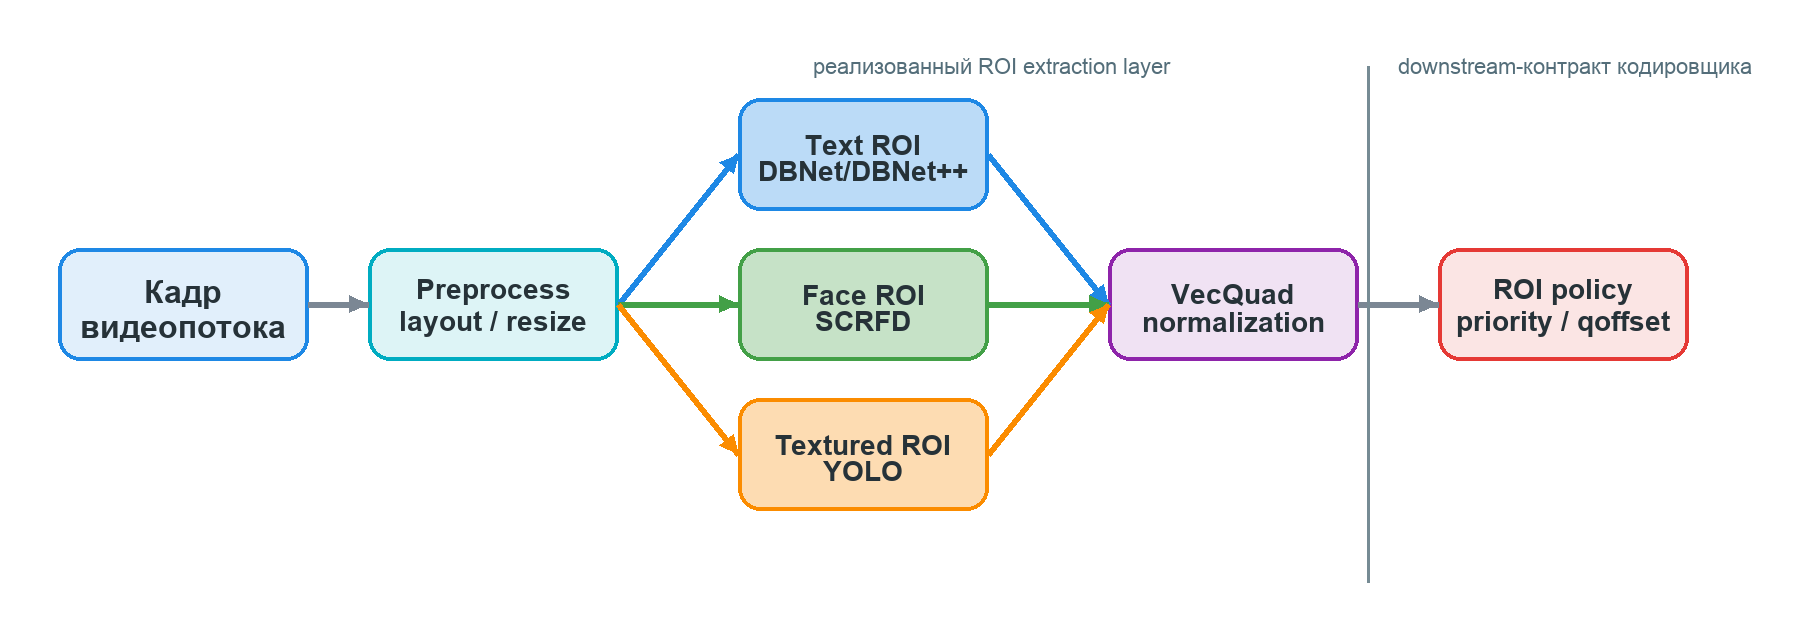
\includegraphics[width=0.96\linewidth]{ch03-architecture/fig01_architecture_three_modes.png}
\caption{Архитектура IDet: единый ROI extraction layer объединяет text ROI, face ROI и textured ROI, после чего формирует приоритеты для кодировщика.}
\label{fig:architecture}
\end{figure}

\chapter{Формальная постановка задачи ROI-aware оптимизации}
\section{Ограниченная оптимизация качества}
В работе задача улучшения качества видео формулируется как ограниченная оптимизация. Пусть $B$ --- доступный битрейт, $T$ --- допустимая задержка анализа кадра, $C$ --- вычислительный бюджет, $\theta$ --- параметры ROI-детектора и политики кодирования. Тогда целевую постановку можно записать так:
\begin{equation}
\max_{\theta} \; \mathbb{E}\left[ Q_{\roi}(F; \theta) \right]
\quad
\text{при условиях}\quad
R(F;\theta) \leq B, \quad L(F;\theta) \leq T, \quad C(F;\theta) \leq C_{\max}.
\label{eq:constrained_opt}
\end{equation}
Здесь $R$ --- фактический расход битрейта, $L$ --- задержка обработки кадра, $C$ --- стоимость вычислений, а $Q_{\roi}$ --- ROI-взвешенное качество. В отличие от лабораторной постановки, где можно максимизировать только mAP, в данной работе важна системная метрика: улучшение качества должно быть достигнуто без выхода за latency budget.

\section{Бюджет площади ROI}
Если защищать слишком большую часть кадра, кодировщик потеряет возможность перераспределять биты. Поэтому вводится ограничение на долю защищенной площади:
\begin{equation}
\frac{\left|\bigcup_{i=1}^{N} R_i\right|}{|F|} \leq \alpha,
\label{eq:area_budget}
\end{equation}
где $\alpha$ --- максимально допустимая доля кадра, например $0.15$--$0.35$ в зависимости от типа контента. Это ограничение принципиально важно для практического стриминга: ROI-aware кодирование не должно превращаться в кодирование всего кадра с повышенным качеством.

\section{Временная стабильность ROI}
Для видео важна не только точность областей в отдельном кадре, но и их стабильность во времени. Если ROI резко прыгает между соседними кадрами, это может привести к мерцанию качества. Для сглаживания confidence используется рекуррентная формула
\begin{equation}
\hat{s}_{t} = \lambda \hat{s}_{t-1} + (1-\lambda) s_t,
\label{eq:smoothing}
\end{equation}
где $s_t$ --- текущая уверенность детектора, $\hat{s}_t$ --- сглаженная уверенность, $\lambda \in [0,1]$ --- коэффициент памяти. Дополнительно можно ввести штраф за нестабильность:
\begin{equation}
P_{flicker} = \frac{1}{T-1}\sum_{t=2}^{T} \left(1 - \operatorname{IoU}(R_t, R_{t-1})\right).
\label{eq:flicker}
\end{equation}
Чем выше $P_{flicker}$, тем сильнее меняется ROI между кадрами и тем выше риск визуального мерцания.

\section{От ROI к qoffset кодировщика}
FFmpeg предоставляет структуру \texttt{AVRegionOfInterest}, где область задается координатами и параметром \texttt{qoffset}; отрицательное значение qoffset означает повышение качества кодирования внутри ROI \cite{ffmpeg_roi}. На уровне фильтров аналогичная идея доступна через \texttt{addroi}: фильтр не изменяет пиксели кадра, а прикрепляет к нему metadata об областях интереса для последующего кодирования \cite{ffmpeg_addroi}. Упрощенная формула преобразования приоритета $p_i$ в смещение QP может быть записана как
\begin{equation}
\Delta QP_i = -\gamma \cdot p_i \cdot (QP_{\max} - QP_{\min}),
\label{eq:qoffset}
\end{equation}
где $p_i \in [0,1]$ --- нормированный приоритет области, а $\gamma$ --- коэффициент силы защиты. Формула~\eqref{eq:qoffset} не навязывает конкретную реализацию кодировщика, но описывает общий принцип: чем важнее область, тем сильнее отрицательное смещение QP.

\section{Метрики детекции}
Для модели textured ROI используются стандартные метрики object detection: precision, recall, F1, AP, mAP@0.5 и mAP@0.5:0.95 \cite{ultra_metrics}. Они вычисляются по формулам
\begin{equation}
\operatorname{Precision} = \frac{TP}{TP + FP}, \qquad
\operatorname{Recall} = \frac{TP}{TP + FN},
\label{eq:precision_recall}
\end{equation}
\begin{equation}
F_1 =
2\cdot
\frac{\operatorname{Precision}\cdot \operatorname{Recall}}
{\operatorname{Precision}+\operatorname{Recall}}.
\label{eq:f1}
\end{equation}
В контексте ROI-задачи recall особенно важен: пропуск значимой области одежды хуже, чем неточная классификация типа одежды, потому что цель детектора текстурированных ROI --- не модная аналитика, а защита визуально богатой области от агрессивного сжатия.

\chapter{Проектирование IDet и трехрежимного ROI-конвейера}
\section{IDet как инженерное ядро работы}
IDet --- это CPU-first C++ библиотека для детекции и нормализации областей интереса \cite{idet}. В данной работе она рассматривается как центральный инженерный результат: задача библиотеки состоит не в том, чтобы обучить единственную модель, а в том, чтобы связать несколько специализированных детекторов с видеокодировщиком через устойчивый геометрический контракт. Реальный публичный контракт IDet возвращает список четырехугольников \texttt{VecQuad}; типизация ROI, приоритеты и \texttt{qoffset} являются следующим слоем интеграции, который строится поверх этой геометрии при подключении кодировщика. Такой дизайн отделяет компьютерное зрение от политики кодирования и делает систему расширяемой: можно заменить модель текста, лиц или текстурированных областей, не меняя downstream-логику распределения качества.

Архитектурно IDet опирается на несколько принципов. Во-первых, критический путь должен работать на CPU без Python-зависимости, поскольку облачный transcoding часто выполняется на CPU-пулах или в средах, где GPU является дорогим и разделяемым ресурсом. Во-вторых, модели должны приводиться к deployable формату ONNX, а инференс должен выполняться через ONNX Runtime \cite{onnx,onnxruntime}. В-третьих, графы моделей должны проходить оптимизацию: ONNX Runtime поддерживает уровни graph optimizations и online/offline режимы, что позволяет отделить подготовку артефакта от исполнения в сервисе \cite{ort_graph_optim}. В-четвертых, входные и выходные буферы должны быть переиспользуемыми; механизм I/O Binding в ONNX Runtime позволяет заранее связать входы и выходы с нужным размещением и уменьшить количество копирований \cite{ort_iobinding}.

\begin{table}[H]
\centering
\caption{Основные модули библиотеки IDet}
\label{tab:idet_modules}
\small
\begin{tabularx}{\linewidth}{@{}p{0.27\linewidth}p{0.24\linewidth}Y@{}}
\toprule
Модуль & Ответственность & Выходной результат \\
\midrule
Frame input layer & Прием кадра, проверка формата, масштабирование и подготовка рабочего представления. & Нормализованный кадр или набор плиток. \\
Preprocessing layer & Letterbox, resize, нормализация каналов, преобразование layout и заполнение входных tensor buffers. & Готовые входные буферы для ONNX Runtime. \\
Model adapters & Обертки над text, face и texture detectors; скрывают формат выходов конкретной модели. & Сырые кандидаты: box, score, class/kind. \\
Post-processing layer & Thresholding, декодирование координат, NMS, stitching плиток и обратное преобразование координат. & Кандидаты ROI в координатах исходного кадра. \\
ROI integration layer & Добавление типа ROI, приоритета, area cap и temporal smoothing поверх геометрии \texttt{VecQuad}. & Упорядоченный список ROI metadata для кодировщика. \\
Encoder adapter & Преобразование ROI metadata в qoffset/ROI side data или fallback-политику. & Encoder guidance для видеокодировщика. \\
Benchmark layer & Измерение latency, числа ROI, площади ROI, числа аллокаций и стабильности результатов. & p50/p95/p99, отчеты и диагностические метрики. \\
\bottomrule
\end{tabularx}
\end{table}

\begin{figure}[H]
\centering
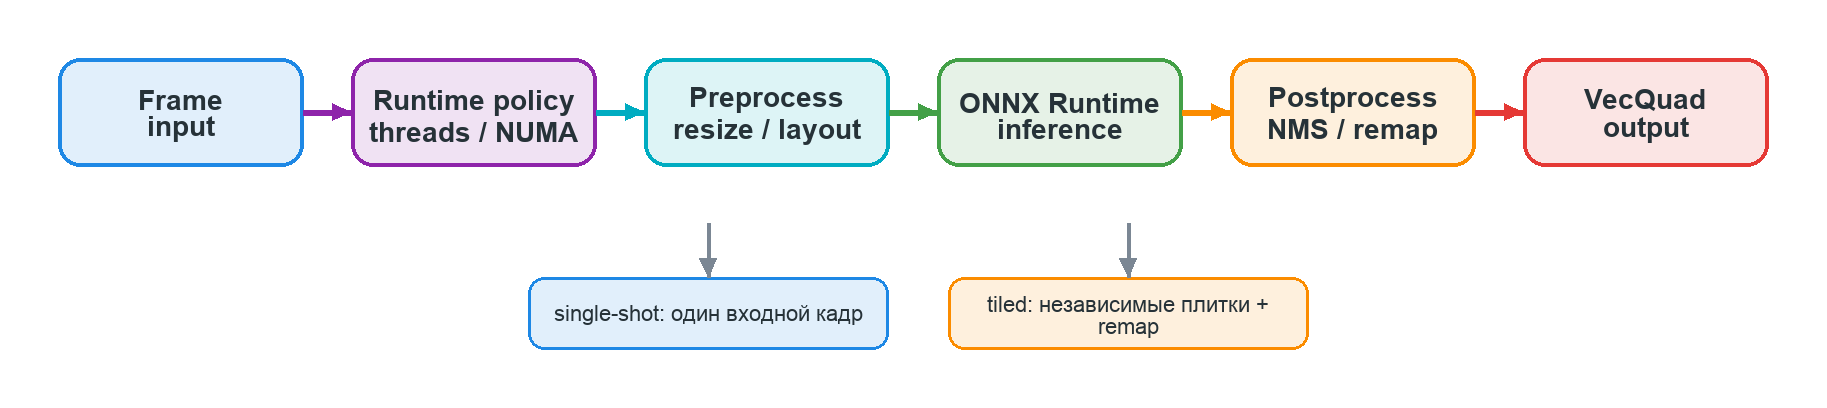
\includegraphics[width=0.96\linewidth]{ch03-architecture/fig02_idet_runtime_pipeline.png}
\caption{Runtime path IDet для одного кадра: подготовка изображения, CPU-инференс, tiled/single post-processing и возврат списка \texttt{VecQuad}.}
\label{fig:idet_runtime}
\end{figure}

\section{Жизненный цикл обработки кадра}
Жизненный цикл кадра в IDet начинается до запуска нейросетевой модели. Сначала система получает кадр в исходном разрешении, проверяет формат пикселей и выбирает режим обработки: полный кадр, downscale, tiled inference или повторное использование ROI с предыдущего кадра. Затем выполняется предобработка, включая letterbox/resize и приведение данных к формату, ожидаемому конкретной ONNX-моделью.

После инференса каждый движок декодирует выходы своей модели. Text engine преобразует probability map DBNet-like модели в quadrilateral detections, SCRFD engine декодирует multi-head face outputs, а YOLO engine преобразует raw или in-graph-NMS outputs в четырехугольники. Публичный слой возвращает \texttt{VecQuad}; следующий интеграционный слой должен добавить тип области, приоритет, ограничение суммарной площади и temporal smoothing. Последним шагом encoder adapter переводит такую ROI metadata в qoffset или другой backend-specific hint.

\begin{table}[H]
\centering
\caption{Жизненный цикл кадра в IDet}
\label{tab:frame_lifecycle}
\small
\begin{tabularx}{\linewidth}{@{}p{0.08\linewidth}p{0.26\linewidth}Y@{}}
\toprule
Шаг & Этап & Смысл этапа \\
\midrule
1 & Frame acquisition & Получение кадра и фиксация его размеров, timestamp и pixel format. \\
2 & Work plan & Выбор режима обработки: полный кадр, плитки, пропуск тяжелого детектора или перенос ROI. \\
3 & Preprocessing & Подготовка входных буферов: resize/letterbox, нормализация, layout conversion. \\
4 & Inference & Выполнение одной или нескольких ONNX Runtime sessions с контролируемым числом потоков. \\
5 & Model post-processing & Декодирование выходов моделей, thresholding, NMS, stitching и обратное масштабирование координат. \\
6 & ROI integration & Добавление типа ROI, сортировка, слияние пересечений, area cap и temporal smoothing поверх \texttt{VecQuad}. \\
7 & Encoder guidance & Преобразование ROI в qoffset/side data или fallback-параметры кодировщика. \\
8 & Telemetry & Запись latency, числа ROI, площади ROI и диагностической информации. \\
\bottomrule
\end{tabularx}
\end{table}

\section{Ответственность адаптеров детекторов}
Adapter в IDet отвечает за преобразование конкретной модели в общий контракт библиотеки. Он не должен принимать решения о том, какие ROI важнее для кодировщика; это ответственность ROI manager. Такой принцип уменьшает связность: модель текста может быть заменена с DBNet на DBNet++, модель лиц --- на другую SCRFD-конфигурацию, а детектор текстурированных ROI --- на более тяжелую YOLO-модель без изменения downstream-слоя.

\begin{table}[H]
\centering
\caption{Ответственность адаптеров IDet}
\label{tab:adapter_responsibilities}
\small
\begin{tabularx}{\linewidth}{@{}p{0.23\linewidth}p{0.30\linewidth}Y@{}}
\toprule
Adapter & Внутренняя ответственность & Что не входит в ответственность \\
\midrule
Text adapter & Предобработка под DBNet/DBNet++, декодирование text maps, polygon/box extraction, фильтрация по confidence. & Глобальный приоритет текста относительно лица и textured ROI. \\
Face adapter & Resize/normalize под SCRFD, декодирование anchors/candidates, NMS лиц, нормализация confidence. & Решение о qoffset и ограничение общей площади ROI. \\
Texture adapter & YOLO-preprocessing, декодирование box/class outputs, NMS, remap координат из letterbox-пространства. & Интерпретация классов одежды как политик кодирования. \\
Encoder adapter & Преобразование ROI metadata в FFmpeg ROI side data, qoffset-map или fallback-параметры. & Запуск детекторов и изменение outputs моделей. \\
\bottomrule
\end{tabularx}
\end{table}

\section{Представление ROI}
Фактическое представление результата в публичном API IDet минималистично: библиотека возвращает \texttt{VecQuad}, то есть список четырехугольников в координатах изображения. Внутренние движки при этом оперируют более богатым объектом \texttt{algo::Detection}, где помимо четырех точек сохраняется confidence score, но этот score не экспортируется наружу через публичный \texttt{Detector::detect}. Для интеграции с кодировщиком такого геометрического контракта недостаточно, поэтому в работе отдельно описывается downstream-запись ROI: она должна добавлять к \texttt{Quad} тип области, приоритет и рекомендуемое смещение QP.

\begin{table}[H]
\centering
\caption{Статус компонентов ROI-aware конвейера}
\label{tab:component_status}
\small
\begin{tabularx}{\linewidth}{@{}p{0.28\linewidth}p{0.25\linewidth}Y@{}}
\toprule
Компонент & Статус & Роль в работе \\
\midrule
\texttt{VecQuad} & реализовано в IDet & Текущий публичный геометрический контракт: список четырехугольников в координатах изображения. \\
Text ROI detector & реализовано / интегрировано & Детекция текстовых областей, критичных для читаемости. \\
Face ROI detector & реализовано / интегрировано & Детекция лиц как семантически важных областей кадра. \\
Textured ROI detector & подготовлен через YOLO pipeline & Детекция одежды и фактурированных областей для третьего ROI-режима. \\
RichROI / ROI metadata & downstream-контракт & Расширение геометрии типом области, confidence, приоритетом и подсказкой qoffset. \\
qoffset mapping & проектируемая encoder policy & Преобразование приоритета ROI в управляющий сигнал для кодировщика. \\
Baseline vs ROI-aware quality & экспериментальный протокол & Финальная количественная оценка закодированного потока выполняется отдельной серией экспериментов. \\
\bottomrule
\end{tabularx}
\end{table}

Такое разделение предотвращает смешение уровней реализации. В текущем коде IDet уже существует единый геометрический выход и runtime-инфраструктура для CPU-инференса. Расширенная ROI metadata, приоритеты и qoffset относятся к downstream-интеграции с кодировщиком: они необходимы для полной ROI-aware системы, но не должны описываться как уже существующий публичный API библиотеки.

\section{Владение буферами и горячий путь}
Для real-time видеостриминга важна не только средняя задержка, но и устойчивость p95/p99. Динамические аллокации в критическом пути приводят к джиттеру: отдельные кадры внезапно обрабатываются дольше из-за выделения памяти, освобождения памяти или переразмещения контейнеров. Поэтому IDet должен использовать явную модель владения буферами.

\begin{table}[H]
\centering
\caption{Модель владения буферами в IDet}
\label{tab:buffer_ownership}
\small
\begin{tabularx}{\linewidth}{@{}p{0.24\linewidth}p{0.24\linewidth}Y@{}}
\toprule
Буфер & Владелец & Правило использования \\
\midrule
Decoded frame & Frame input layer & Только чтение после получения кадра; исходное изображение не меняется детекторами. \\
Preprocessed input & Preprocessing layer & Переиспользуется между кадрами одного размера; заполняется перед inference. \\
ONNX input/output tensors & Inference backend & Выделяются при инициализации session или при смене input shape. \\
Candidate arrays & Model adapter & Очищаются и переиспользуются; вместимость растет только вне hot path. \\
NMS workspace & Post-processing layer & Общий временный буфер для сортировки и подавления кандидатов. \\
ROI metadata list & ROI manager / encoder integration layer & Финальный список областей с типом и приоритетом, передаваемый encoder adapter и telemetry layer. \\
\bottomrule
\end{tabularx}
\end{table}

\section{Приоритеты и разрешение конфликтов}
В системе вводится иерархия приоритетов: текст $>$ лицо $>$ textured ROI $>$ фон. Текст получает максимальный приоритет, потому что даже небольшие артефакты делают его нечитаемым. Лицо получает высокий приоритет из-за чувствительности пользователя к искажениям человеческой внешности. Текстурированные поверхности получают средний приоритет: они важны для субъективной детализации, но не должны вытеснять лицо и текст.

\begin{table}[H]
\centering
\caption{Алгоритм слияния ROI}
\label{tab:roi_fusion_algorithm}
\begin{tabularx}{\linewidth}{@{}p{0.08\linewidth}Y@{}}
\toprule
Шаг & Действие \\
\midrule
1 & Получить кандидаты ROI от text adapter, face adapter и texture adapter. \\
2 & Нормировать координаты, confidence и тип области к downstream-записи ROI поверх \texttt{VecQuad}. \\
3 & Удалить кандидаты с confidence ниже порога, зависящего от типа ROI. \\
4 & Отсортировать ROI по приоритету: text $>$ face $>$ texture $>$ background. \\
5 & Объединить сильно пересекающиеся области с учетом IoU и типа области. \\
6 & Ограничить суммарную защищаемую площадь кадра заданным area budget. \\
7 & Применить temporal smoothing к координатам и confidence для уменьшения flickering. \\
8 & Вернуть упорядоченный список ROI metadata для encoder adapter. \\
\bottomrule
\end{tabularx}
\end{table}


\section{Реальный публичный контракт IDet}
Важное архитектурное решение IDet состоит в том, что конкретная модель не протекает в пользовательский код. Публичный слой выбирает задачу и движок через \texttt{Task} и \texttt{EngineKind}, а пользователь получает геометрию областей как \texttt{VecQuad}. Ниже приведен сокращенный фрагмент публичного заголовочного интерфейса библиотеки; он важен для диплома, потому что фиксирует фактическую границу между C++ библиотекой и внешним видеоконвейером.

\begin{lstlisting}[caption={Сокращенный фрагмент публичного API IDet},label={lst:idet_public_api}]
enum class Task : std::uint8_t {
    None = 0,
    Text = 1,
    Face = 2,
    Cloth = 3,
};

enum class EngineKind : std::uint8_t {
    None = 0,
    DBNet = 1,
    SCRFD = 2,
    Yolo = 3,
};

using Quad = std::array<Point2f, 4>;
using VecQuad = std::vector<Quad>;

struct DetectorConfig final {
    Task task = Task::None;
    EngineKind engine = EngineKind::None;
    InferenceOptions infer{};
    RuntimePolicy runtime{};
    std::string model_path{};
    [[nodiscard]] Status validate() const noexcept;
    static DetectorConfig setup(Task task, std::string model_path);
};

class Detector final {
public:
    static Result<Detector> create(const DetectorConfig& config) noexcept;
    Status prepare_binding(int width, int height, int contexts) noexcept;
    Result<VecQuad> detect(const Image& image) noexcept;
    Result<VecQuad> detect_bound(const Image& image, int ctx_idx) noexcept;
};
\end{lstlisting}

Этот контракт задает границы ответственности фактической реализации. Модельно-зависимые детали --- letterbox, layout conversion, нормализация входа, декодирование выходов, thresholding и NMS --- скрыты внутри движков DBNet, SCRFD и YOLO. Downstream-слой, необходимый для ROI-aware кодирования, должен добавлять к возвращенной геометрии тип области, приоритет и \texttt{qoffset}; в текущем исходном коде это не отдельный публичный класс, а проектируемый слой интеграции с кодировщиком.

\section{Downstream-контракт ROI и приоритеты областей}
Унифицированное представление ROI для кодировщика должно содержать не только координаты. Для кодировщика важны тип области, уверенность, приоритет и ожидаемая сила защиты. Поэтому поверх фактического \texttt{VecQuad} в работе вводится downstream-запись ROI, которую можно реализовать в encoder integration layer. Минимальный состав такой записи приведен в таблице~\ref{tab:richroi_contract}; это не утверждение о наличии одноименной структуры в текущем публичном API IDet.

\begin{table}[H]
\centering
\caption{Downstream-контракт ROI metadata между детекторами, ROI manager и encoder adapter}
\label{tab:richroi_contract}
\small
\begin{tabularx}{\linewidth}{@{}p{0.24\linewidth}p{0.24\linewidth}Y@{}}
\toprule
Поле & Пример & Назначение \\
\midrule
\texttt{kind} & \texttt{text}, \texttt{face}, \texttt{texture} & Тип ROI, определяющий приоритет и политику qoffset. \\
\texttt{quad/bbox} & TL--TR--BR--BL или \texttt{x1,y1,x2,y2} & Геометрия области в координатах исходного кадра. \\
\texttt{confidence} & $0.0$--$1.0$ & Уверенность конкретного детектора. \\
\texttt{priority} & $0.0$--$1.0$ & Системный приоритет после учета типа и confidence. \\
\texttt{area} & доля кадра & Используется для area budget и отсечения чрезмерно больших ROI. \\
\texttt{qoffsetHint} & отрицательное значение & Предлагаемое смещение квантования для encoder adapter. \\
\texttt{source} & \texttt{dbnet}, \texttt{scrfd}, \texttt{yolo26n} & Источник ROI для диагностики и ablation study. \\
\texttt{trackId} & целое число или \texttt{none} & Связь ROI между кадрами для temporal smoothing. \\
\bottomrule
\end{tabularx}
\end{table}

Приоритеты должны быть заданы явно. В типичном сценарии текст получает наивысший приоритет, потому что потеря читаемости является критической. Лица также имеют высокий приоритет из-за заметности артефактов. Textured ROI полезны для perceived sharpness, но их приоритет должен быть ниже, чтобы они не вытесняли текст и лица при ограниченном area budget.

\section{Инварианты и отказоустойчивость IDet}
Для производственного конвейера важно определить не только идеальный путь, но и инварианты, которые должны сохраняться при ошибках. IDet должен выдерживать отсутствие модели, пустой список ROI, недоступность native ROI support в кодировщике и временные пики задержки. Поэтому для каждого кадра система должна гарантировать следующие свойства:
\begin{enumerate}[label=\arabic*)]
  \item координаты ROI находятся внутри границ исходного кадра;
  \item суммарная площадь защищаемых областей не превышает заданный бюджет $\alpha$;
  \item пересекающиеся ROI не приводят к конфликтующим qoffset одного и того же блока;
  \item при сбое одного детектора остальные режимы могут продолжить работу;
  \item при превышении latency budget система может временно перейти к переносимым ROI предыдущих кадров или к более дешевой ветке;
  \item отсутствие native ROI support не должно ломать кодирование: encoder adapter обязан перейти к fallback-политике.
\end{enumerate}

Эти инварианты важны для диплома, поскольку показывают, что IDet проектируется не как демонстрационный скрипт, а как слой, который может быть встроен в реальный видеоконвейер с ограничениями по времени, памяти и надежности.

\section{Память, буферы и zero-allocation hot path}
Одним из источников нестабильности p95/p99 является динамическое выделение памяти в горячем пути. Для CPU-first inference это особенно важно: даже если сама нейросеть выполняется быстро, повторяющиеся аллокации входных тензоров, временных массивов NMS или списков кандидатов могут ухудшать хвост задержек. Поэтому IDet должен стремиться к zero-allocation hot path: крупные буферы выделяются на этапе инициализации, а затем переиспользуются.

Практический список буферов включает входной image buffer, tensor input buffer, output buffers ONNX Runtime, временные массивы кандидатов, workspace NMS, массивы для stitching плиток и финальный контейнер \texttt{VecQuad}. Использование ONNX Runtime I/O Binding позволяет заранее связать входы и выходы с выбранными буферами и уменьшить количество лишних копирований между этапами \cite{ort_iobinding}. Это особенно важно для ARM/Kunpeng CPU-only сценариев, где пропускная способность памяти и NUMA locality заметно влияют на tail latency.

\section{Политика потоков}
IDet должен контролировать два уровня параллелизма: внешний уровень обработки кадров/плиток и внутренний уровень потоков ONNX Runtime. Если оба уровня включены без ограничений, возникает oversubscription: несколько пулов потоков конкурируют за одни и те же CPU-ядра, что ухудшает p95/p99 latency. Поэтому политика потоков должна задаваться явно и быть частью конфигурации, а не побочным эффектом backend.

\begin{table}[H]
\centering
\caption{Политика потоков в IDet}
\label{tab:threading_policy}
\small
\begin{tabularx}{\linewidth}{@{}p{0.23\linewidth}p{0.27\linewidth}Y@{}}
\toprule
Уровень & Настраиваемый параметр & Инженерный смысл \\
\midrule
Frame-level parallelism & Число одновременно обрабатываемых кадров. & Увеличивает throughput, но может ухудшить latency отдельного кадра. \\
Tile-level parallelism & Число плиток, обрабатываемых параллельно. & Полезно для крупных кадров, но требует аккуратного stitching. \\
ORT intra-op threads & Число потоков внутри оператора ONNX Runtime. & Влияет на скорость сверточных и матричных операций. \\
ORT inter-op threads & Параллелизм между независимыми узлами графа. & Эффективен не для всех моделей; требует профилирования. \\
Detector sampling rate & Частота запуска каждой ветки ROI. & Позволяет запускать тяжелые детекторы реже и переносить ROI во времени. \\
\bottomrule
\end{tabularx}
\end{table}

\section{Интеграция с кодировщиком}
\begin{figure}[htbp]
\centering
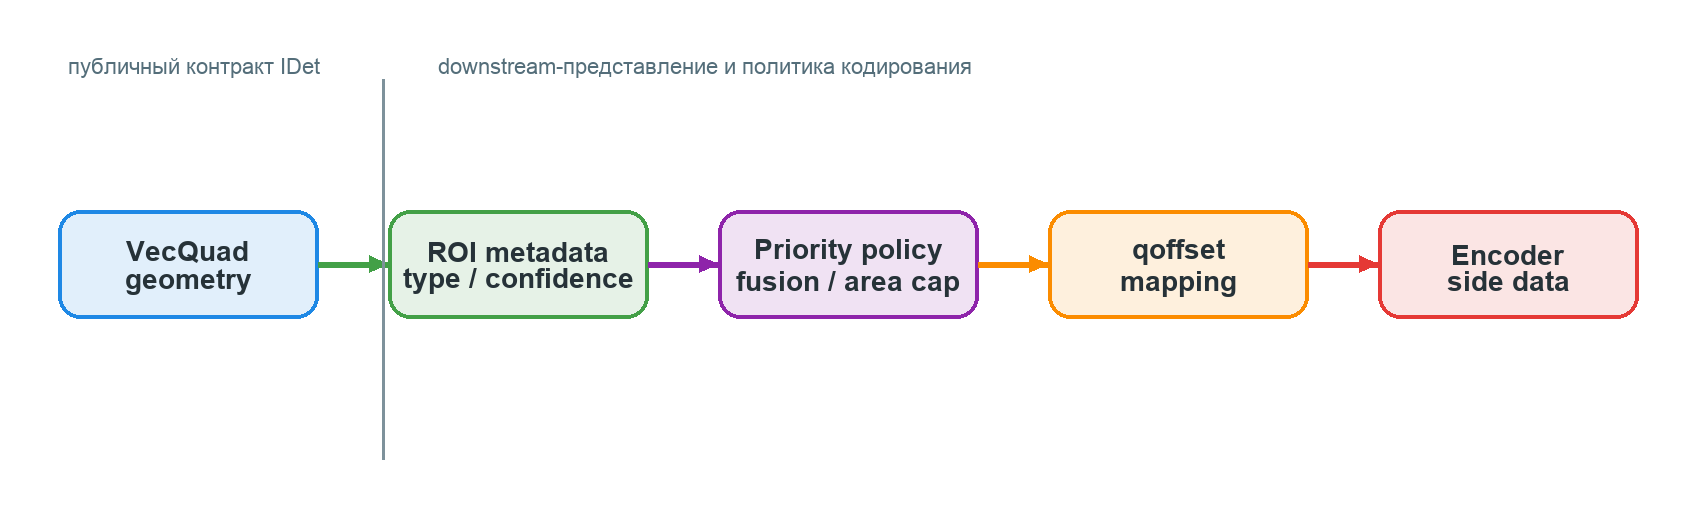
\includegraphics[width=0.96\linewidth]{ch03-architecture/fig15_encoder_mapping.png}
\caption{Преобразование ROI metadata в encoder guidance: ограничение площади, сортировка, qoffset mapping и передача ROI side data.}
\label{fig:encoder_mapping}
\end{figure}

Интеграционный слой должен быть отделен от детекторов. Модель не должна знать, работает ли кодировщик через FFmpeg ROI metadata, adaptive quantization или через fallback-предобработку фона. FFmpeg \texttt{addroi} прикрепляет к кадру metadata об областях интереса, не изменяя пиксели самого кадра, а \texttt{AVRegionOfInterest} задает координаты и qoffset для таких областей \cite{ffmpeg_addroi,ffmpeg_roi}. Это делает encoder adapter естественной границей между компьютерным зрением и кодированием.

\begin{table}[H]
\centering
\caption{Алгоритмический контракт encoder adapter}
\label{tab:encoder_adapter_contract}
\begin{tabularx}{\linewidth}{@{}p{0.23\linewidth}Y@{}}
\toprule
Операция & Семантика \\
\midrule
\texttt{supportsROI} & Проверить, может ли целевой backend принять ROI side data или qoffset-map. \\
\texttt{mapPriority} & Преобразовать приоритет ROI metadata в qoffset или эквивалентный encoder hint. \\
\texttt{applyHints} & Передать кодировщику список ROI после ограничения площади и сортировки. \\
\texttt{fallback} & При отсутствии native ROI support применить альтернативную стратегию: сглаживание фона или conservative AQ settings. \\
\bottomrule
\end{tabularx}
\end{table}

Этот adapter позволяет сохранить модульность: IDet отвечает за поиск областей, ROI manager --- за слияние и стабилизацию, encoder adapter --- за конкретный способ влияния на кодирование.

\chapter{Детектор текстурированных ROI: данные, обучение и экспорт}
\section{Мотивация детекции текстурированных ROI}
ROI-aware видеокодирование часто связывают с лицами и текстом, поскольку эти области имеют очевидную семантическую ценность. Однако в пользовательском видео существенную часть ощущения резкости формируют текстуры: одежда ведущего, ткань, ворс, узор, мелкие регулярные структуры и декоративные поверхности. При сильном сжатии такие области теряют высокочастотные детали и превращаются в сглаженные пятна. Поэтому textured ROI рассматривается как третий режим IDet: он не конкурирует с text ROI и face ROI, а расширяет систему на визуально богатые области, для которых трудно задать простые эвристики.

Для этой ветки используется объектный детектор семейства YOLO, обученный на согласованной таксономии одежды. Выбор объектного детектора, а не общей saliency-модели, связан с инженерной управляемостью: bbox легко преобразовать в ROI кодировщика, ошибки можно анализировать через AP и confusion matrix, а latency можно профилировать на CPU.

\section{Конвейер подготовки и обучения YOLO-модели}
Для обучения детектора текстурированных ROI используется отдельный проект generic YOLO training pipeline \cite{pipeline}. Его задача --- обеспечить полный цикл подготовки и проверки модели: конвертацию датасетов, согласование таксономии, проверку разметки, аудит bbox-геометрии, построение статистики, запуск обучения, оценку и экспорт deployable артефактов. Поддержка ONNX-экспорта важна, поскольку Ultralytics рассматривает export mode как основной путь переноса обученной модели в форматы для deployment, включая ONNX \cite{ultra_export,ultra_onnx}. Логика pipeline представлена на рисунке~\ref{fig:generic_pipeline}.

\begin{figure}[H]
\centering
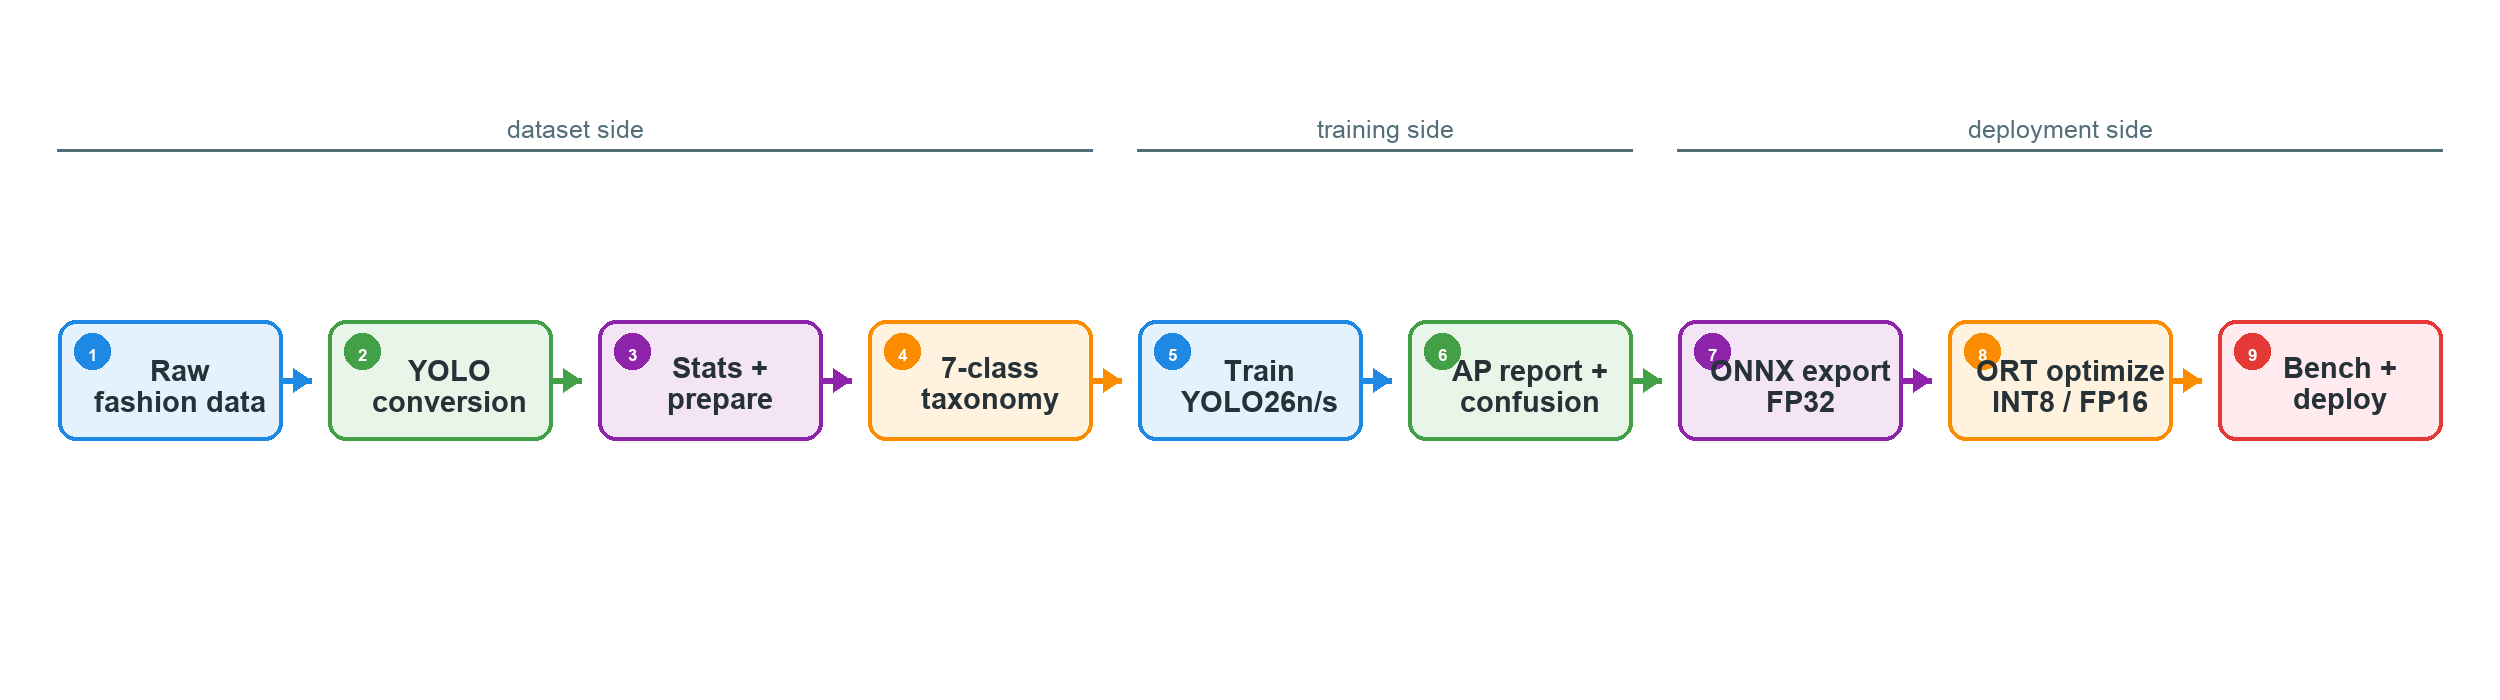
\includegraphics[width=0.96\linewidth]{ch05-yolo-results/fig03_generic_yolo_pipeline.png}
\caption{Generic YOLO pipeline для детектора текстурированных ROI: подготовка датасетов, согласование таксономии, обучение, оценка и этап экспорта PT-to-ONNX.}
\label{fig:generic_pipeline}
\end{figure}

\begin{figure}[H]
\centering
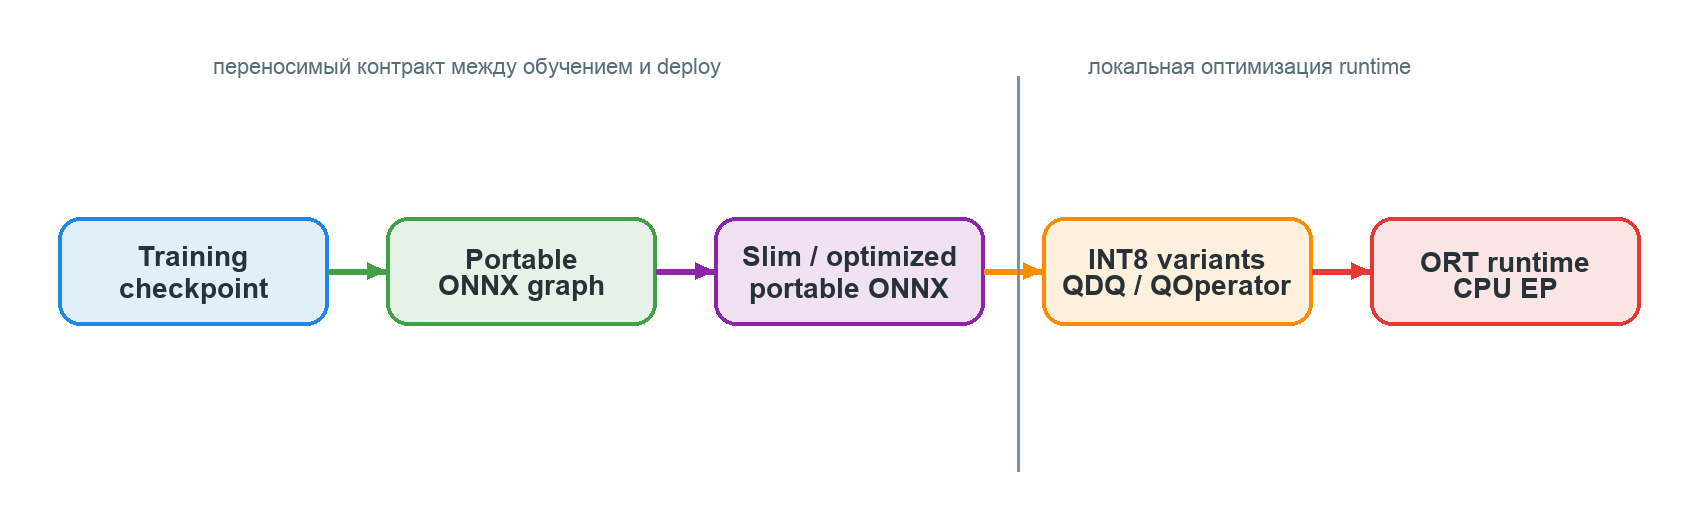
\includegraphics[width=0.96\linewidth]{ch05-yolo-results/fig20_pt_onnx_ort_deployment.png}
\caption{Путь подготовки deployable артефакта: от training checkpoint к переносимому ONNX и исполнению через ONNX Runtime CPU Execution Provider.}
\label{fig:pt_onnx_ort}
\end{figure}

Использовались два исходных датасета: DeepFashion2 и Fashionpedia. DeepFashion2 содержит изображения одежды с аннотациями для detection, segmentation, landmarks и retrieval \cite{deepfashion2}. Fashionpedia построена вокруг fashion ontology и содержит категории одежды, части одежды и fine-grained attributes \cite{fashionpedia}. Оба датасета были переведены в YOLO-формат, после чего из исходных таксономий выделены 7 ключевых классов, согласованных между источниками.

\section{Контракт PT-to-ONNX артефакта}
Отдельным модулем generic YOLO pipeline является stage экспорта обученной PT-модели в ONNX. Этот этап нужен не для отчетности, а для замыкания цикла между обучением и IDet: библиотека не должна зависеть от Python training framework, поэтому в runtime передается стабильный ONNX-артефакт с известной формой входа, набором выходов и настройками оптимизации. В ONNX Runtime такой артефакт может дополнительно проходить graph optimizations, включая устранение лишних узлов, fusion операций и оптимизации layout в зависимости от выбранного уровня \cite{ort_graph_optim}.

\begin{table}[H]
\centering
\caption{Контракт PT-to-ONNX артефакта для детектора текстурированных ROI}
\label{tab:pt_to_onnx_contract}
\small
\begin{tabularx}{\linewidth}{@{}p{0.27\linewidth}Y@{}}
\toprule
Элемент контракта & Требование \\
\midrule
Входной артефакт & Лучший training checkpoint, полученный после обучения YOLO-модели на согласованной таксономии. \\
Экспортируемый формат & ONNX model artifact, совместимый с ONNX Runtime CPU Execution Provider. \\
Размер входа & Фиксированный или явно задокументированный dynamic input shape; размер должен совпадать с preprocessing в IDet. \\
Параметры экспорта & \texttt{format=onnx}, выбранный \texttt{opset}, режим \texttt{dynamic}, \texttt{simplify}, batch size и флаг встроенного NMS фиксируются в отчете pipeline. \\
Проверка корректности & Сравнение выходов PT и ONNX на калибровочных изображениях: shape, диапазоны confidence, число кандидатов и близость координат. \\
Проверка переносимости & Portable ONNX не должен содержать target-specific узлы ONNX Runtime layout optimization, например \texttt{com.microsoft.nchwc::Conv}; такие файлы допустимы только как отдельные ORT-optimized artifacts для конкретной машины. \\
Оптимизация & Сохранение версии до оптимизации и версии после ORT graph optimization для воспроизводимого benchmark. \\
Метаданные & Версия pipeline, дата экспорта, dataset yaml, names/classes, hash весов и параметры preprocessing. \\
Интеграция & Артефакт регистрируется как texture adapter model и используется IDet без обращения к Python. \\
\bottomrule
\end{tabularx}
\end{table}

\section{Единая 7-классовая таксономия}

Целевая таксономия включает классы: \texttt{top\_sleeved}, \texttt{outerwear}, \texttt{top\_sleeveless}, \texttt{shorts}, \texttt{trousers}, \texttt{skirt}, \texttt{dress}. Выбор классов обусловлен задачей textured ROI: эти классы покрывают основные области одежды, которые чаще всего занимают значительную часть кадра и имеют воспринимаемую фактуру.

\section{Аудит датасетов после конвертации}
В таблице~\ref{tab:dataset_summary} приведена сводка по трем конфигурациям: DeepFashion2, Fashionpedia и объединенному набору. Во всех случаях отсутствуют пустые разметочные записи, отсутствующие метки, «осиротевшие» метки и нечитаемые изображения. Это является важным инженерным результатом: качество модели начинается не с архитектуры, а с корректности подготовленного корпуса.

\begin{table}[H]
\centering
\caption{Сводная статистика датасетов после конвертации в YOLO-формат}
\label{tab:dataset_summary}
\small
\begin{tabularx}{\linewidth}{lrrrrr}
\toprule
Датасет & Images & Instances & Train img & Val img & Test img \\
\midrule
DeepFashion2 & 224114 & 364675 & 179291 & 22411 & 22412 \\
Fashionpedia & 45445 & 74724 & 36356 & 4544 & 4545 \\
Объединенный набор & 269559 & 439399 & 234516 & 32347 & 2696 \\
\bottomrule
\end{tabularx}
\end{table}

\begin{figure}[H]
\centering
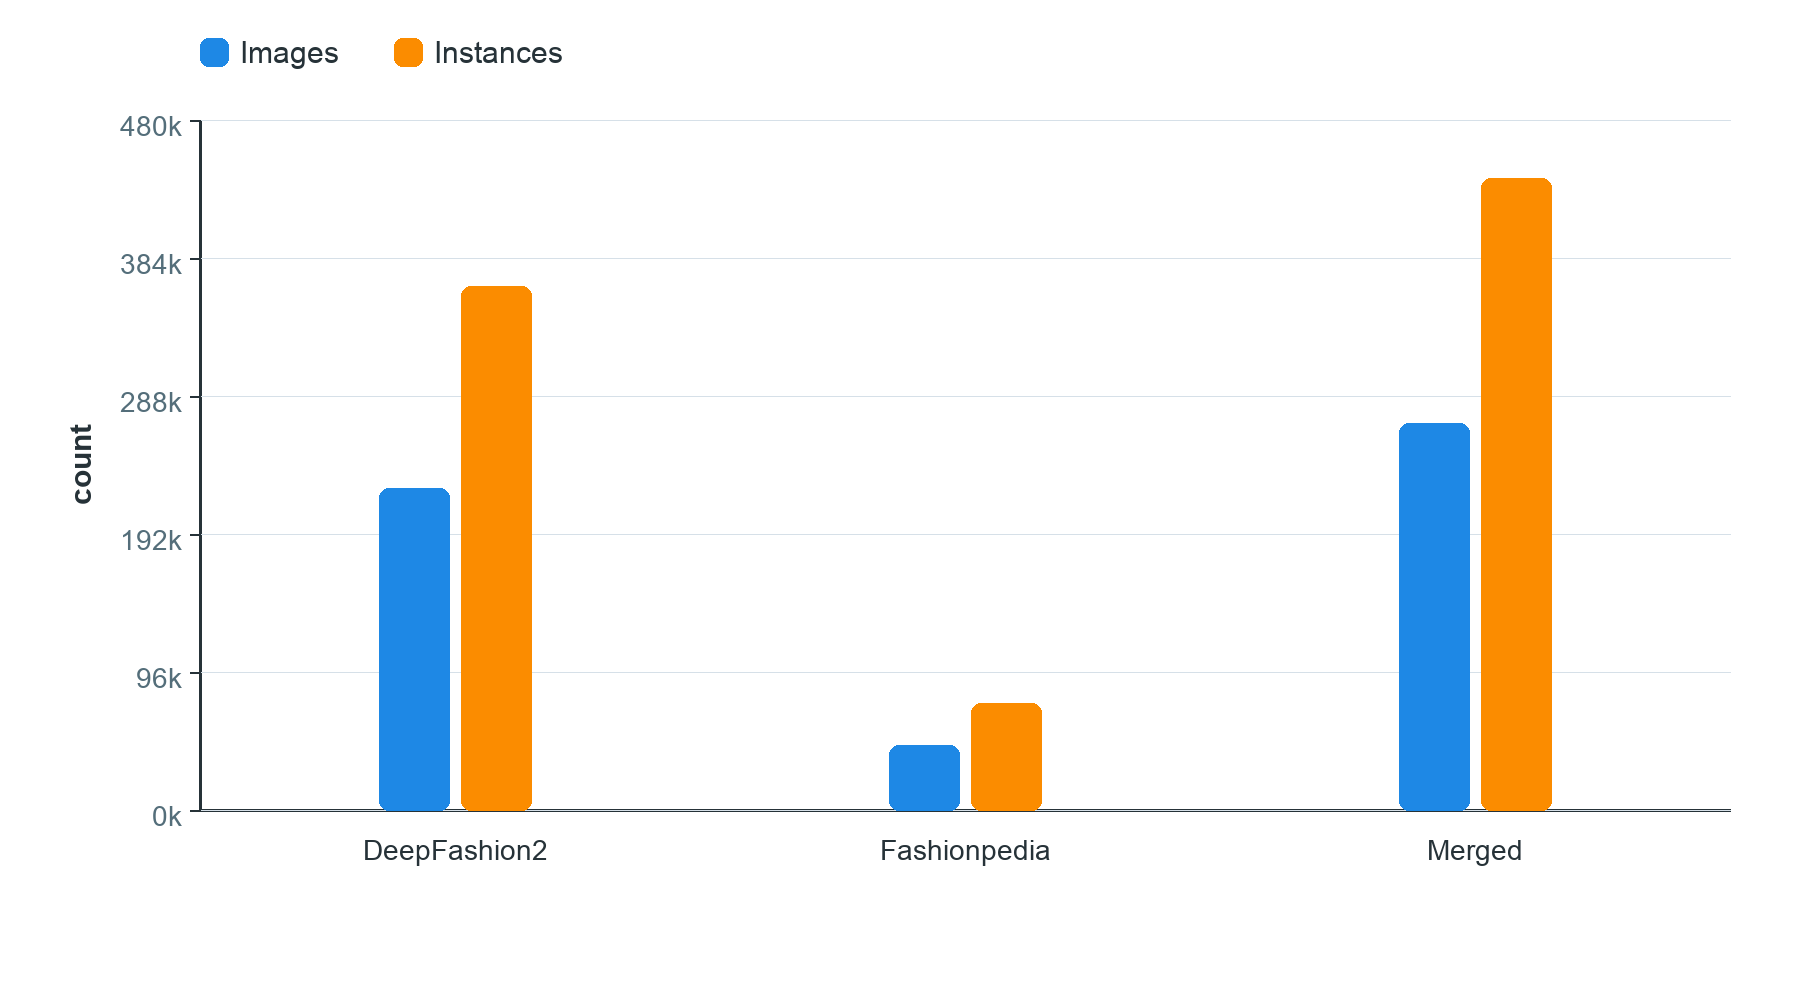
\includegraphics[width=0.86\linewidth]{ch04-datasets/fig04_dataset_scale.png}
\caption{Сравнение масштаба датасетов после приведения к общей таксономии.}
\label{fig:dataset_scale}
\end{figure}

\begin{figure}[H]
\centering
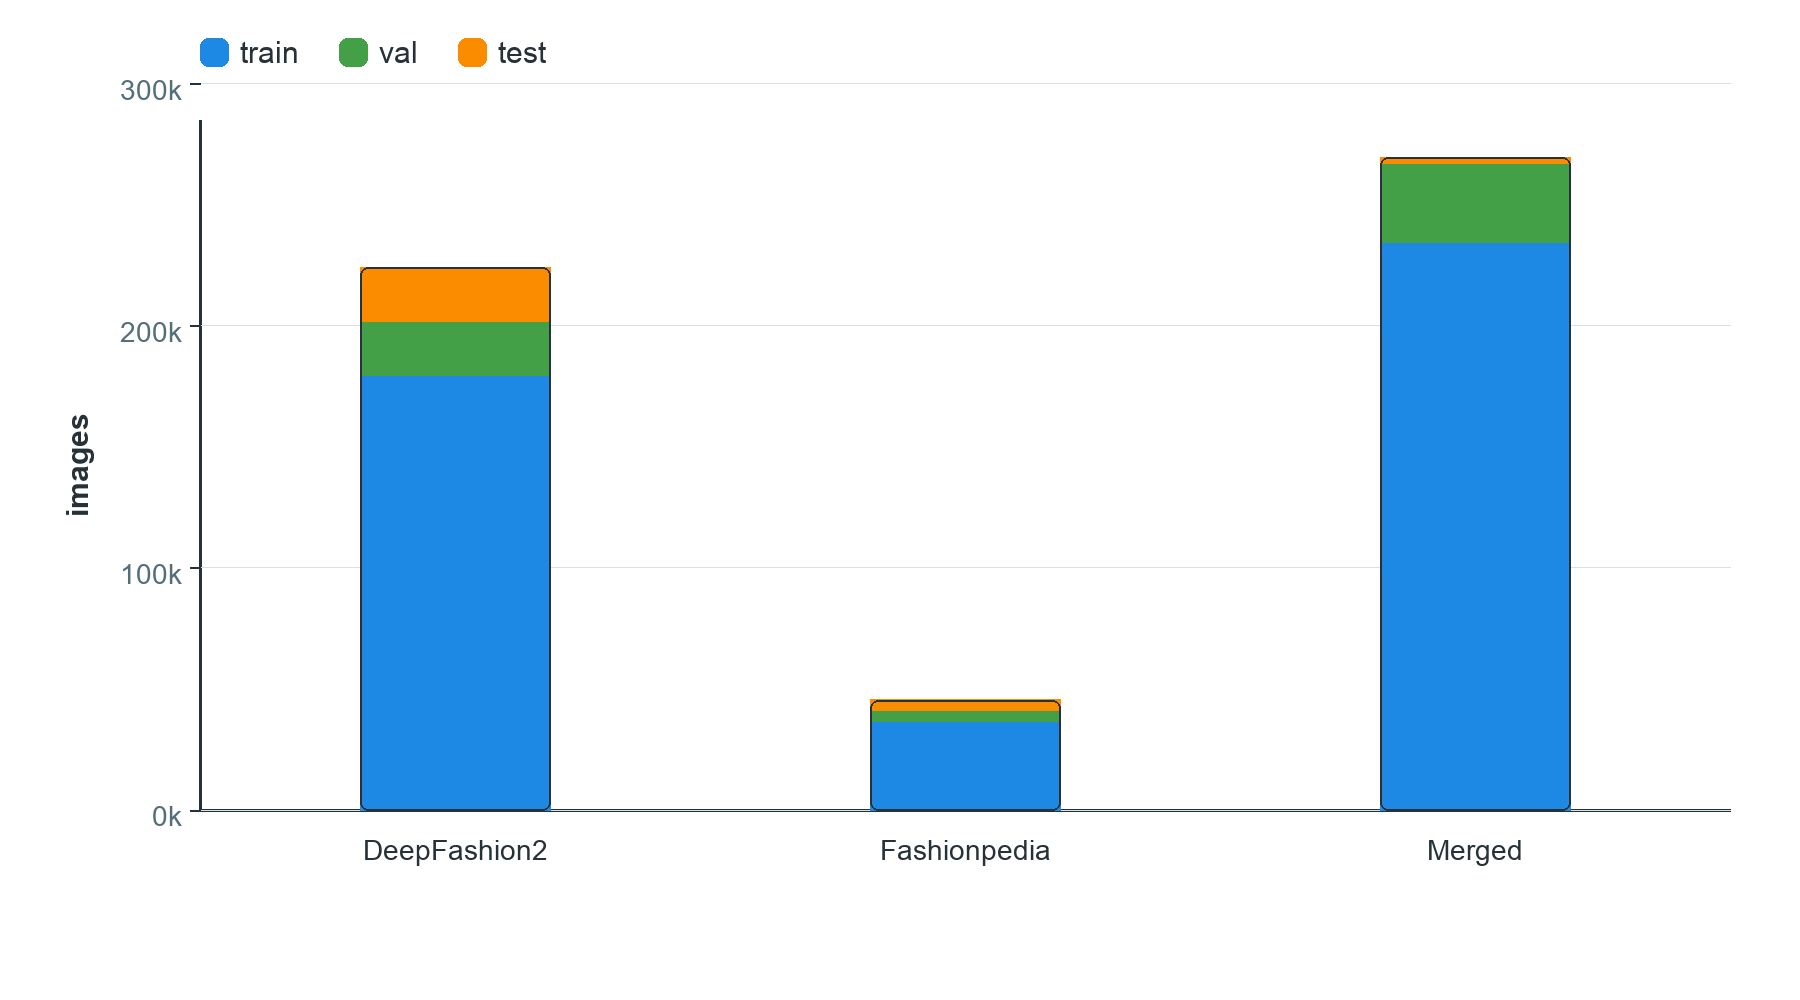
\includegraphics[width=0.86\linewidth]{ch04-datasets/fig05_split_distribution.png}
\caption{Распределение изображений по train/val/test-разбиениям для DeepFashion2, Fashionpedia и объединенного набора.}
\label{fig:split_distribution}
\end{figure}

\section{Дисбаланс классов}
Класс \texttt{top\_sleeved} доминирует во всех конфигурациях. В DeepFashion2 он составляет 126230 объектов, в Fashionpedia --- 24803, а в объединенном наборе --- 151033. При этом в Fashionpedia класс \texttt{top\_sleeveless} содержит только 741 объект, что создает сильный imbalance. После объединения редкие классы получают больше примеров, а отношение крупнейшего класса к минимальному становится существенно мягче.

\begin{table}[H]
\centering
\caption{Распределение объектов по классам в объединенном датасете}
\label{tab:merged_classes}
\small
\begin{tabularx}{\linewidth}{lrrrr}
\toprule
Класс & Train & Val & Test & Total \\
\midrule
\texttt{top\_sleeved} & 132382 & 17116 & 1535 & 151033 \\
\texttt{dress} & 67265 & 9833 & 813 & 77911 \\
\texttt{trousers} & 67226 & 9631 & 844 & 77701 \\
\texttt{shorts} & 36958 & 6203 & 484 & 43645 \\
\texttt{skirt} & 35909 & 6163 & 493 & 42565 \\
\texttt{outerwear} & 20407 & 4556 & 325 & 25288 \\
\texttt{top\_sleeveless} & 17033 & 3925 & 298 & 21256 \\
\bottomrule
\end{tabularx}
\end{table}

\begin{figure}[H]
\centering
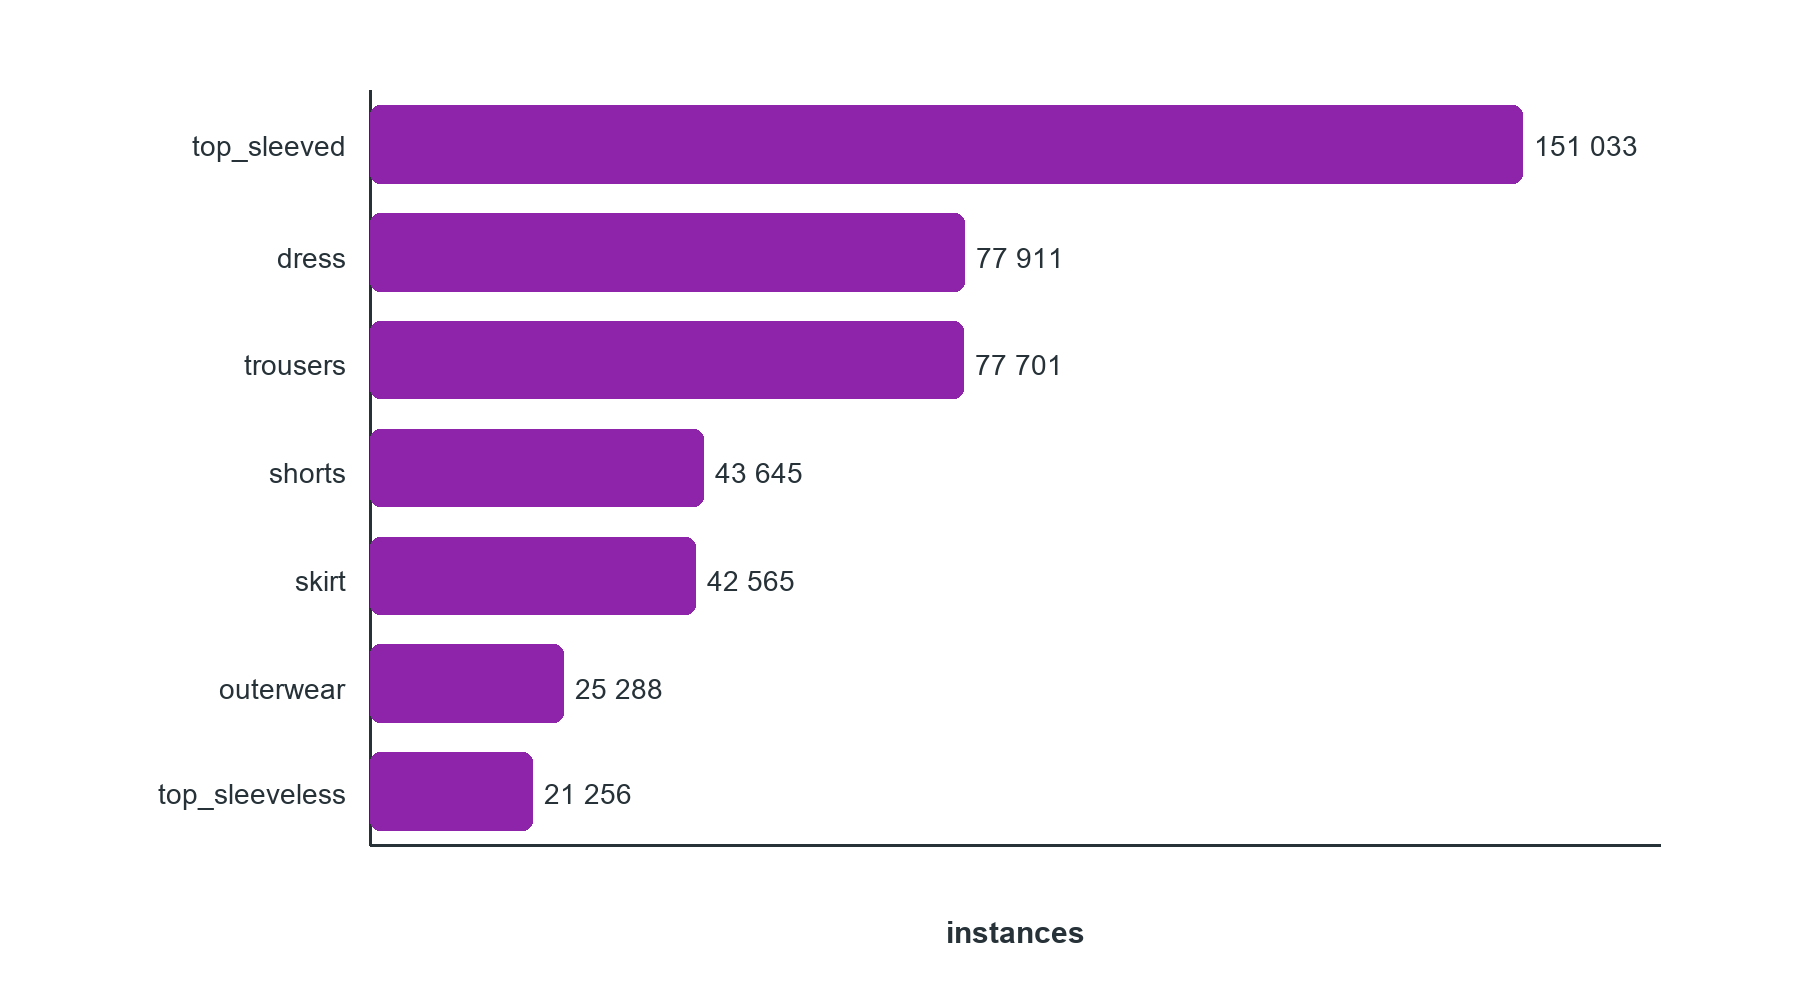
\includegraphics[width=0.90\linewidth]{ch04-datasets/fig06_class_distribution.png}
\caption{Распределение объектов по классам в объединенном датасете.}
\label{fig:class_distribution}
\end{figure}

\section{Геометрия изображений и bbox}
Fashion-домены имеют выраженную вертикальную ориентацию. Для DeepFashion2 средний размер изображения составляет примерно $602.5\times756.8$ на train split, для Fashionpedia --- $755.3\times986.1$, для merged --- $628.3\times795.7$. Центры bbox устойчиво находятся около центра кадра: для merged train средний bbox center равен $(0.5008, 0.5237)$, а средняя площадь bbox --- $0.2709$.

Это свойство имеет два следствия. С одной стороны, модель может переобучиться на центральное расположение объектов. Поэтому при обучении применялись современные аугментации, особенно геометрические: shift, scale, perspective/affine transforms и mosaic-like augmentations \cite{ultra_aug}. С другой стороны, центральность bbox полезна для реального streaming-контента с человеком в кадре: одежда ведущего часто действительно находится в центральной области, а значит textured ROI можно стабилизировать во времени.

\begin{figure}[H]
\centering
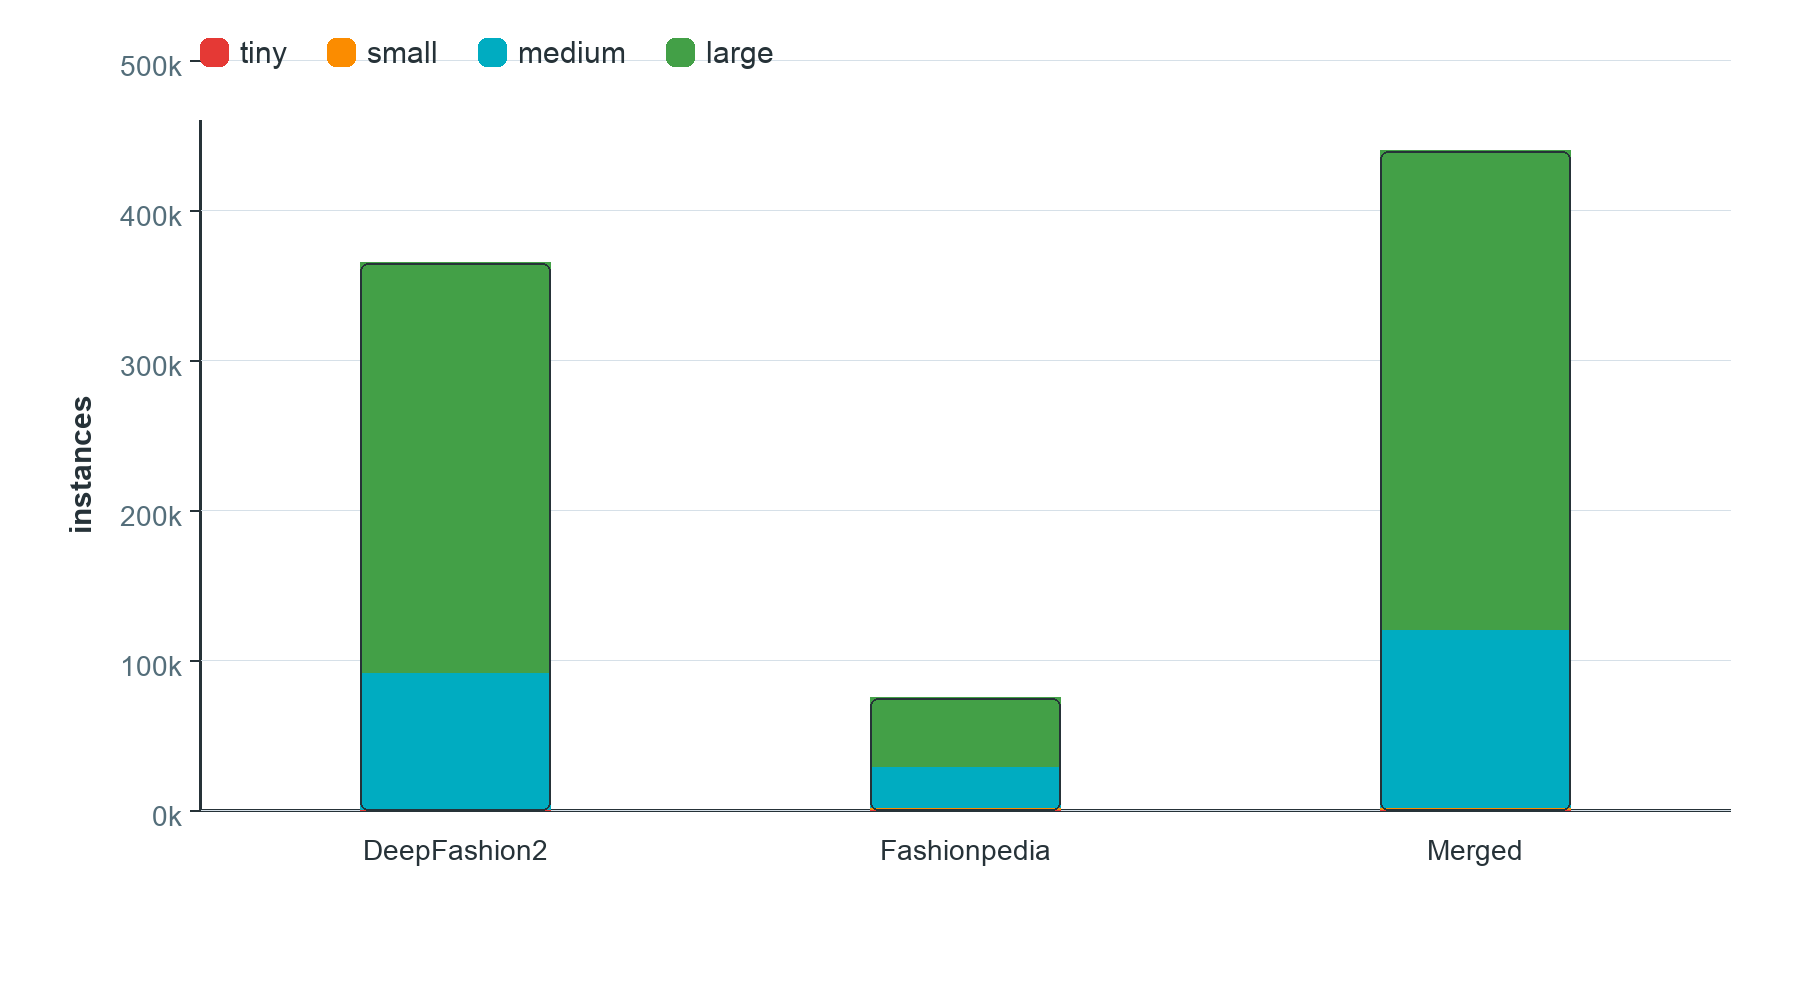
\includegraphics[width=0.86\linewidth]{ch04-datasets/fig07_bbox_area_composition.png}
\caption{Распределение bbox по размерным группам после конвертации в YOLO-формат.}
\label{fig:bbox_area}
\end{figure}

\section{Режимы обучения}
В работе рассматривались следующие режимы:
\begin{enumerate}[label=\arabic*)]
  \item обучение только на DeepFashion2-7c;
  \item обучение только на Fashionpedia-7c;
  \item transfer learning: DeepFashion2 $\rightarrow$ Fashionpedia;
  \item обучение на объединенном наборе DeepFashion2 и Fashionpedia;
  \item сравнение YOLO26n и YOLO26s.
\end{enumerate}

Итоговый выбор сделан в пользу YOLO26n на объединенном наборе. YOLO26s местами давал более высокие метрики, включая mAP@0.5:0.95 выше 0.84, но был тяжелее. Для ВКР важнее не абсолютный максимум mAP, а возможность интеграции в IDet с жестким CPU-бюджетом. Поэтому метрики обучения рассматриваются как первый уровень проверки; окончательный вывод о пригодности для real-time режима требует отдельного CPU-бенчмарка экспортированного ONNX-артефакта вместе с pre/post-processing.


\section{Артефакты ONNX Runtime и квантизация}
После обучения модель должна пройти отдельный этап проверки как deployable artifact. Для этого недостаточно сохранить лучший training checkpoint: необходимо убедиться, что экспортированный ONNX-граф совместим с ONNX Runtime CPU Execution Provider, не содержит непереносимых внутренних layout-операторов и сохраняет ожидаемые формы выходов. ONNX Runtime поддерживает несколько классов оптимизации графа и отдельные механизмы квантизации, включая QDQ-представление и QOperator-представление \cite{ort_graph_optim,ort_quantization}. Однако наличие INT8-артефакта само по себе не гарантирует ускорение: итоговая скорость зависит от kernels, структуры графа, overhead dequantization и целевой архитектуры CPU.

В рамках pipeline целесообразно сохранять следующие артефакты:
\begin{enumerate}[label=\arabic*)]
  \item лучший training checkpoint;
  \item исходный экспортированный ONNX-граф;
  \item slimmed ONNX после удаления лишних узлов;
  \item FP32 ONNX для baseline CPU inference;
  \item QDQ INT8 ONNX для сравнения с FP32;
  \item QOperator INT8 ONNX, если он поддерживается CPU EP и не ухудшает качество;
  \item inspection report с количеством операторов и проверкой доменов;
  \item benchmark report с p50/p90/p95/p99 для каждого артефакта.
\end{enumerate}

Особое внимание нужно уделять операциям домена \texttt{com.microsoft.nchwc}. Они могут появляться в результате внутренних оптимизаций ONNX Runtime для конкретной машины. Такой граф полезен как target-specific optimized artifact, но не должен подменять portable ONNX contract между training pipeline и IDet. В дипломе это различие важно, потому что воспроизводимый deploy artifact должен быть переносимым, а локальная оптимизация под Kunpeng или другой CPU должна описываться как отдельный этап.

\begin{table}[H]
\centering
\caption{Классификация ONNX/ORT-артефактов в pipeline}
\label{tab:onnx_artifact_taxonomy}
\small
\begin{tabularx}{\linewidth}{@{}p{0.25\linewidth}p{0.25\linewidth}Y@{}}
\toprule
Артефакт & Роль & Основная проверка \\
\midrule
Raw ONNX & Базовый экспорт из training framework. & Shape inputs/outputs, opset, отсутствие ошибок загрузки. \\
Slimmed ONNX & Упрощенный переносимый граф. & Сохранение численной близости и структуры outputs. \\
FP32 ONNX & Baseline deploy model. & p99 latency, memory footprint, operator counts. \\
QDQ INT8 ONNX & Квантизованный граф с Quantize/DeQuantize узлами. & Quality regression, dequantization overhead, CPU kernels. \\
QOperator INT8 ONNX & Граф с квантизованными операторами. & Поддержка операторов CPU EP и отсутствие fallback на медленные пути. \\
ORT optimized artifact & Локально оптимизированный артефакт. & Привязка к runtime/CPU, недопустимость как portable contract. \\
\bottomrule
\end{tabularx}
\end{table}

\chapter{Экспериментальные результаты YOLO-моделей на объединенной таксономии}
\section{Граница экспериментальных выводов}
В этой главе приведены результаты обучения и валидации YOLO26n как детектора текстурированных ROI. Эти результаты подтверждают качество object detection на подготовленной 7-классовой таксономии, но сами по себе не доказывают ускорение IDet и не доказывают рост качества видеокодирования. Для таких выводов нужны отдельные CPU-only прогоны ONNX Runtime с p50/p90/p95/p99 latency и отдельный эксперимент кодирования с одинаковым битрейтом. Такое разделение важно, потому что высокая mAP и низкая задержка полного ROI pipeline являются разными свойствами системы.

\section{Аппаратная конфигурация}
Обучение выполнялось на рабочей станции с NVIDIA RTX 4090 24GB, Intel Core i7-13700 и 64GB RAM. Такая конфигурация позволила запускать обучение YOLO26n/YOLO26s с тяжелыми аугментациями и большим merged dataset. RTX 4090 имеет 24 GB видеопамяти, что делает ее практичной для обучения современных моделей компьютерного зрения \cite{nvidia4090}.

\begin{table}[H]
\centering
\caption{Аппаратная конфигурация обучения}
\label{tab:hardware}
\begin{tabularx}{\linewidth}{lY}
\toprule
Компонент & Значение \\
\midrule
GPU & NVIDIA RTX 4090, 24 GB VRAM \\
CPU & Intel Core i7-13700 \\
RAM & 64 GB \\
Модели & YOLO26n, YOLO26s \\
Выбранная модель & YOLO26n \\
Критерий выбора & качество при минимальной вычислительной стоимости для CPU-first IDet \\
\bottomrule
\end{tabularx}
\end{table}

\section{Итоговые метрики}
Итоговые метрики YOLO26n на объединенной 7-классовой таксономии приведены в таблице~\ref{tab:yolo_metrics}. По результатам валидационного отчета модель достигла mAP@0.5 = 0.938 и mAP@0.5:0.95 = 0.818 при precision = 0.903 и recall = 0.873. С точки зрения object detection это сильный результат, особенно если учитывать, что модель выбрана как легкий вариант для последующей CPU-интеграции. При этом в доступных отчетах нет подтвержденного значения оптимального F1-порога, поэтому он не используется как численный вывод.

\begin{table}[H]
\centering
\caption{Итоговые метрики YOLO26n на объединенной 7-классовой таксономии}
\label{tab:yolo_metrics}
\begin{tabularx}{\linewidth}{lrY}
\toprule
Метрика & Значение & Интерпретация \\
\midrule
Precision & 0.903 & Модель сохраняет высокий уровень точности по валидационному отчету. \\
Recall & 0.873 & Модель находит большую часть релевантных областей одежды. \\
mAP@0.5 & 0.938 & Высокое качество при стандартном IoU-пороге. \\
mAP@0.5:0.95 & 0.818 & Устойчивое качество при строгих порогах локализации. \\
\bottomrule
\end{tabularx}
\end{table}

\section{Поклассовая точность детектора}
Поклассовая AP показывает, что модель наиболее уверенно распознает \texttt{trousers}, \texttt{dress}, \texttt{top\_sleeved}, \texttt{shorts} и \texttt{skirt}. Более сложными являются \texttt{top\_sleeveless} и \texttt{outerwear}. Это ожидаемо: \texttt{top\_sleeveless} является менее представленным и визуально близким к другим верхним классам, а \texttt{outerwear} часто пересекается с \texttt{top\_sleeved} и \texttt{dress}. Для поклассового сравнения в основном тексте достаточно графика: он показывает как мягкий AP@0.5, так и более строгий AP@0.5:0.95.

\begin{figure}[H]
\centering
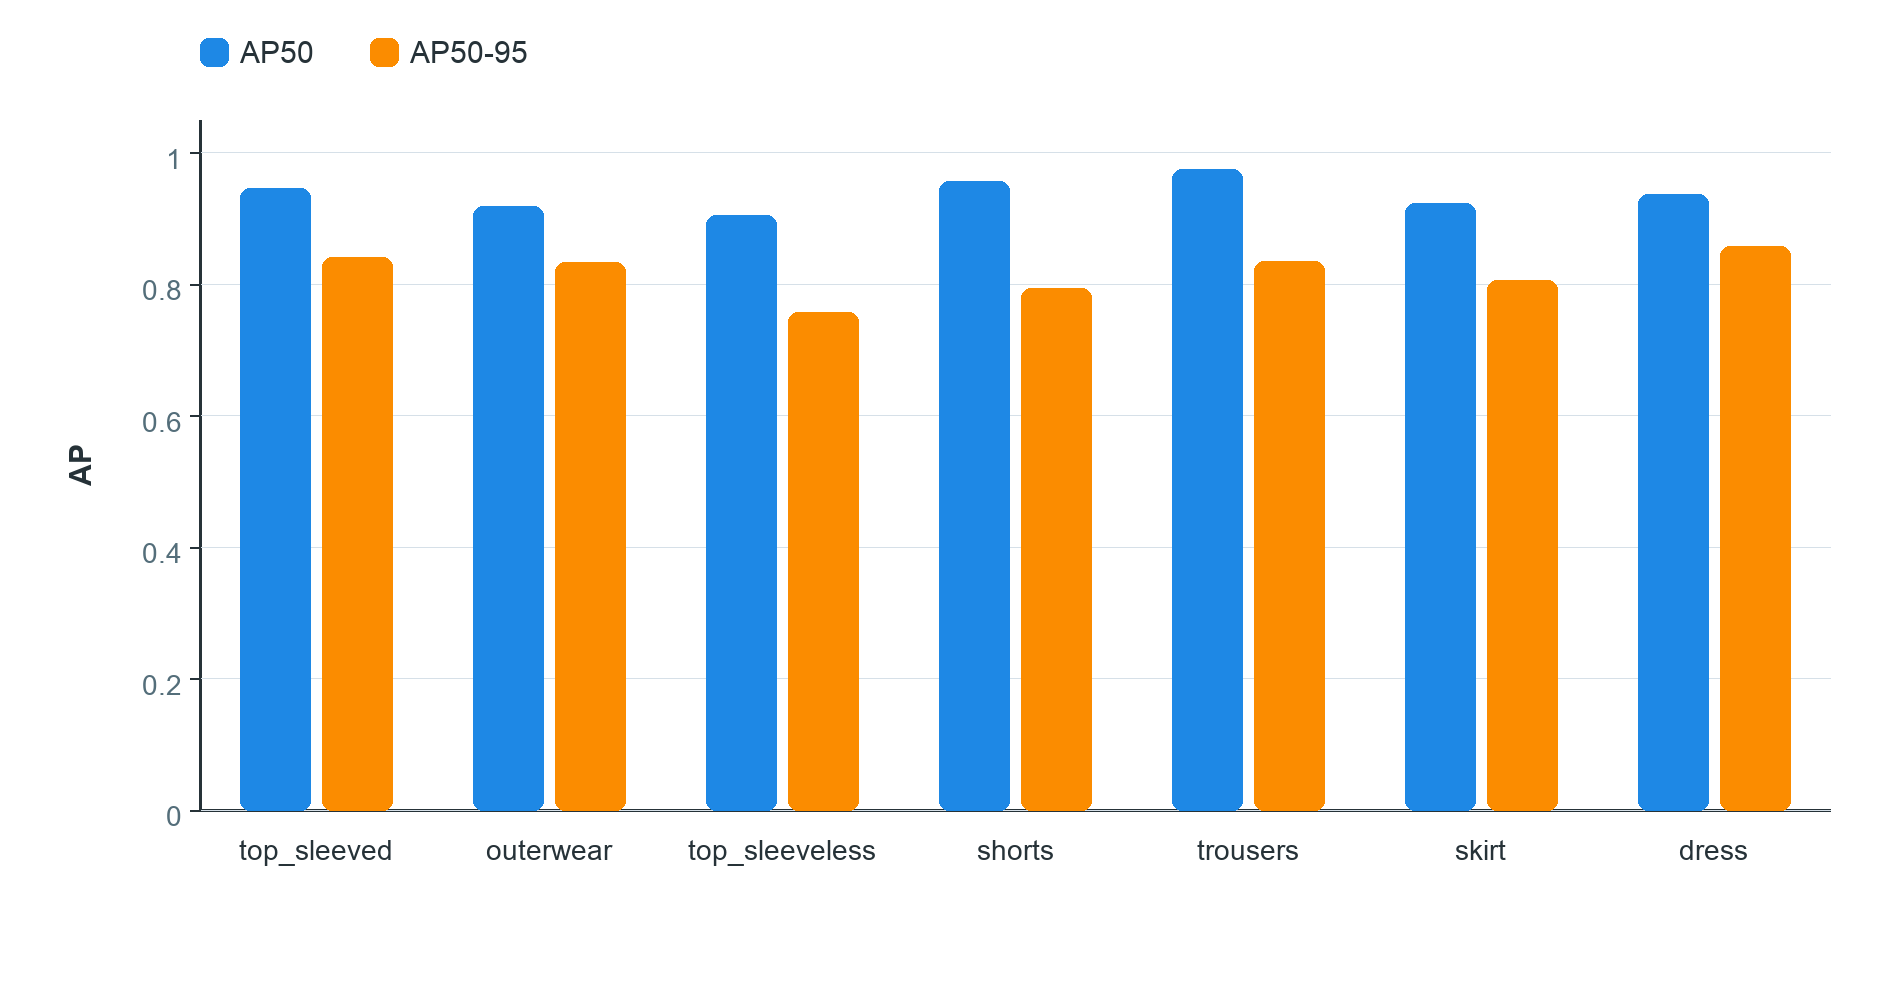
\includegraphics[width=0.86\linewidth]{ch05-yolo-results/fig09_yolo26n_per_class_ap.png}
\caption{Поклассовая AP@0.5 для детектора текстурированных ROI.}
\label{fig:per_class_ap}
\end{figure}

\section{Строгая поклассовая AP и сравнение моделей}
Для ROI-задачи важна не только AP при IoU 0.5, но и устойчивость локализации при более строгих порогах. На рисунке~\ref{fig:per_class_ap_strict} показана поклассовая mAP@0.5:0.95 для YOLO26n на объединенном наборе. Самым слабым классом остается \texttt{top\_sleeveless} с AP@0.5:0.95 = 0.758; это согласуется с дисбалансом датасета и визуальной близостью sleeveless-вещей к другим верхним категориям. При этом \texttt{dress}, \texttt{top\_sleeved}, \texttt{trousers} и \texttt{outerwear} сохраняют значения выше 0.83, что достаточно для роли ROI proposal detector.

\begin{figure}[H]
\centering
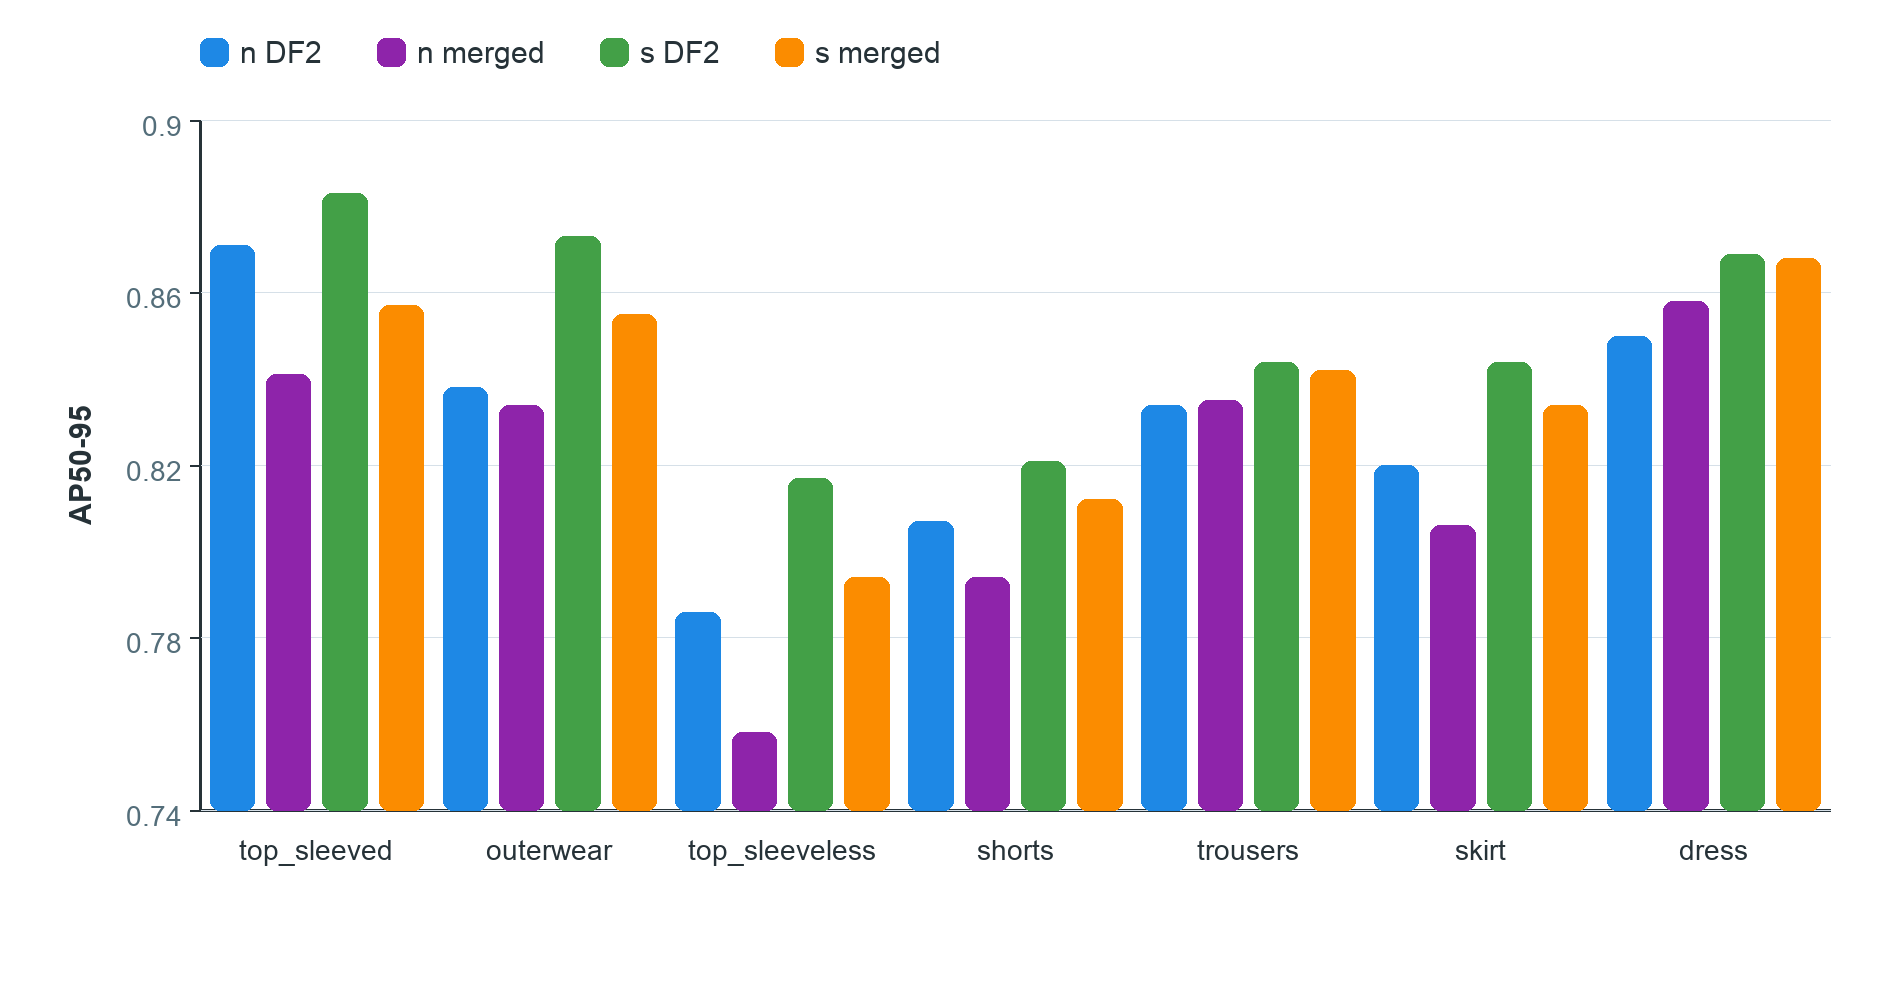
\includegraphics[width=0.86\linewidth]{ch05-yolo-results/fig10_per_class_ap_strict.png}
\caption{Поклассовая AP@0.5:0.95 для YOLO26n на объединенной 7-классовой таксономии.}
\label{fig:per_class_ap_strict}
\end{figure}

Сравнение четырех запусков показывает ожидаемый компромисс. YOLO26s имеет около 9.47 млн параметров и 20.5 GFLOPs против 2.38 млн параметров и 5.2 GFLOPs у YOLO26n, то есть примерно четырехкратную вычислительную стоимость по валидационным отчетам. На DeepFashion2 это дает рост mAP@0.5:0.95 с 0.829 до 0.850. На объединенном датасете отчеты показывают 0.818 для YOLO26n и 0.837 для YOLO26s; это сравнение нужно трактовать осторожно, потому что число validation images/instances в двух отчетах различается. Тем не менее общий вывод устойчив: более тяжелая модель дает умеренный прирост качества, но хуже соответствует CPU-first роли IDet.

\begin{figure}[H]
\centering
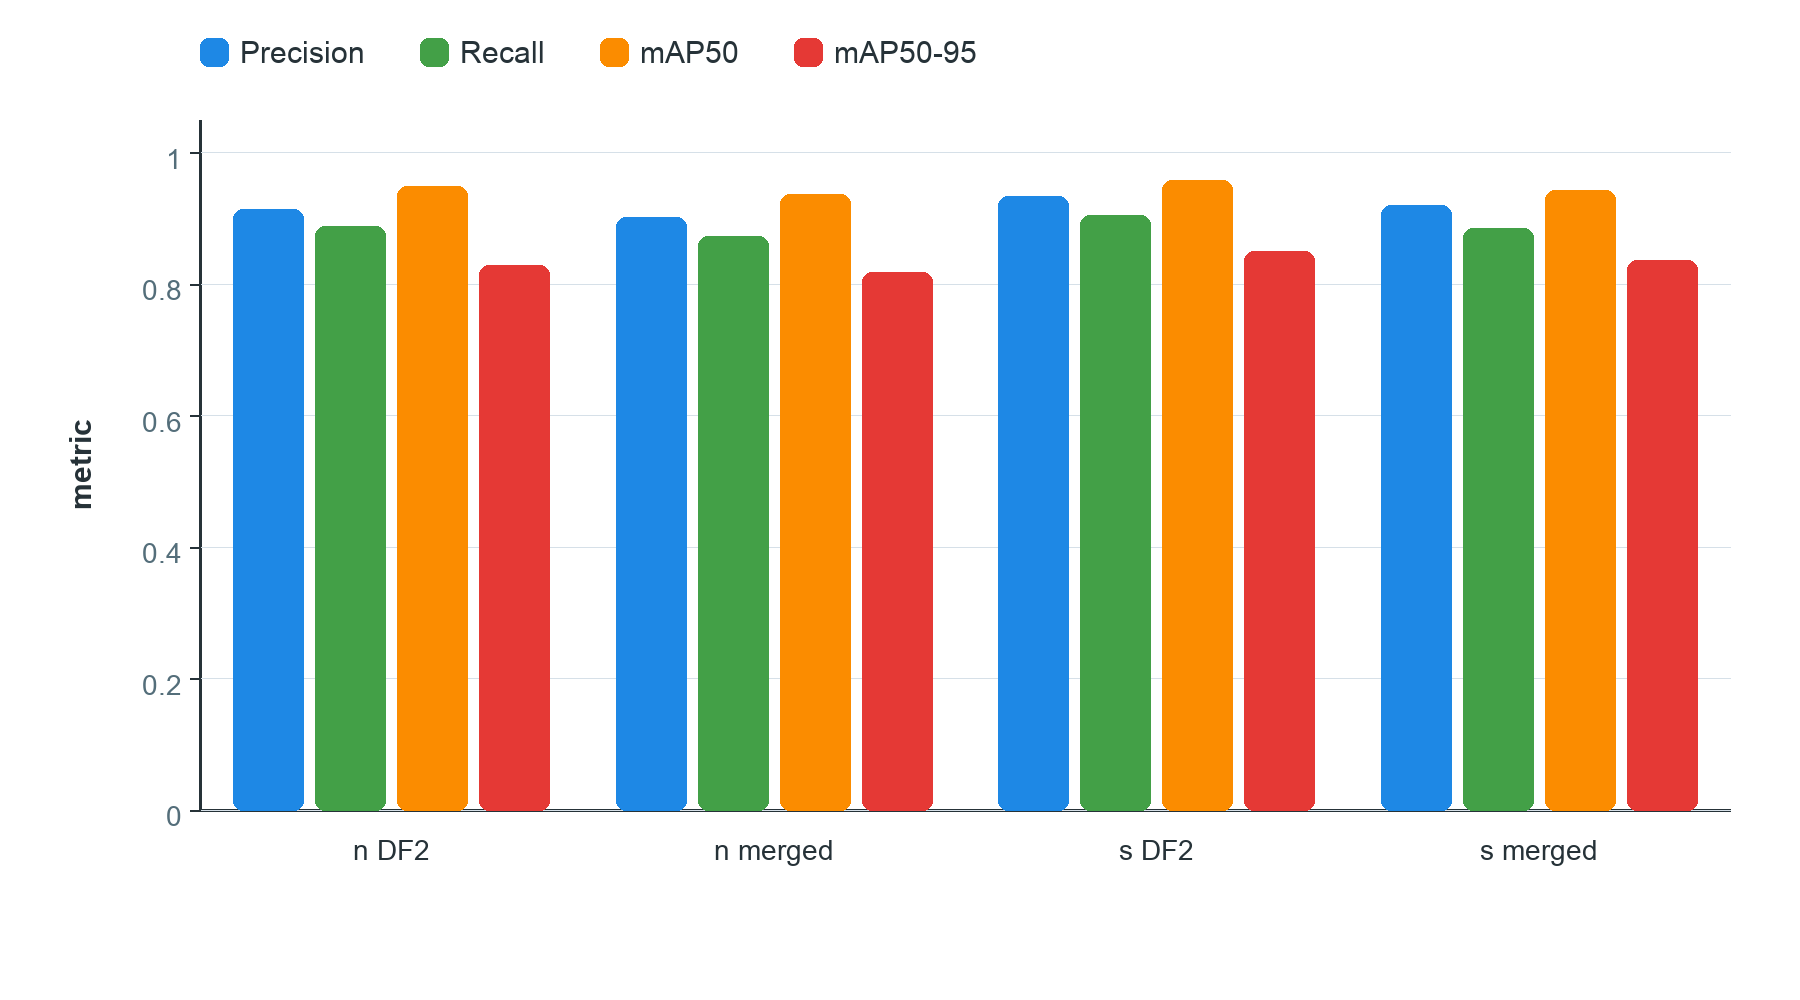
\includegraphics[width=0.90\linewidth]{ch05-yolo-results/fig11_model_comparison.png}
\caption{Сравнение precision, recall, mAP@0.5 и mAP@0.5:0.95 для YOLO26n/YOLO26s на сохраненных validation summaries.}
\label{fig:model_comparison}
\end{figure}

\begin{figure}[H]
\centering
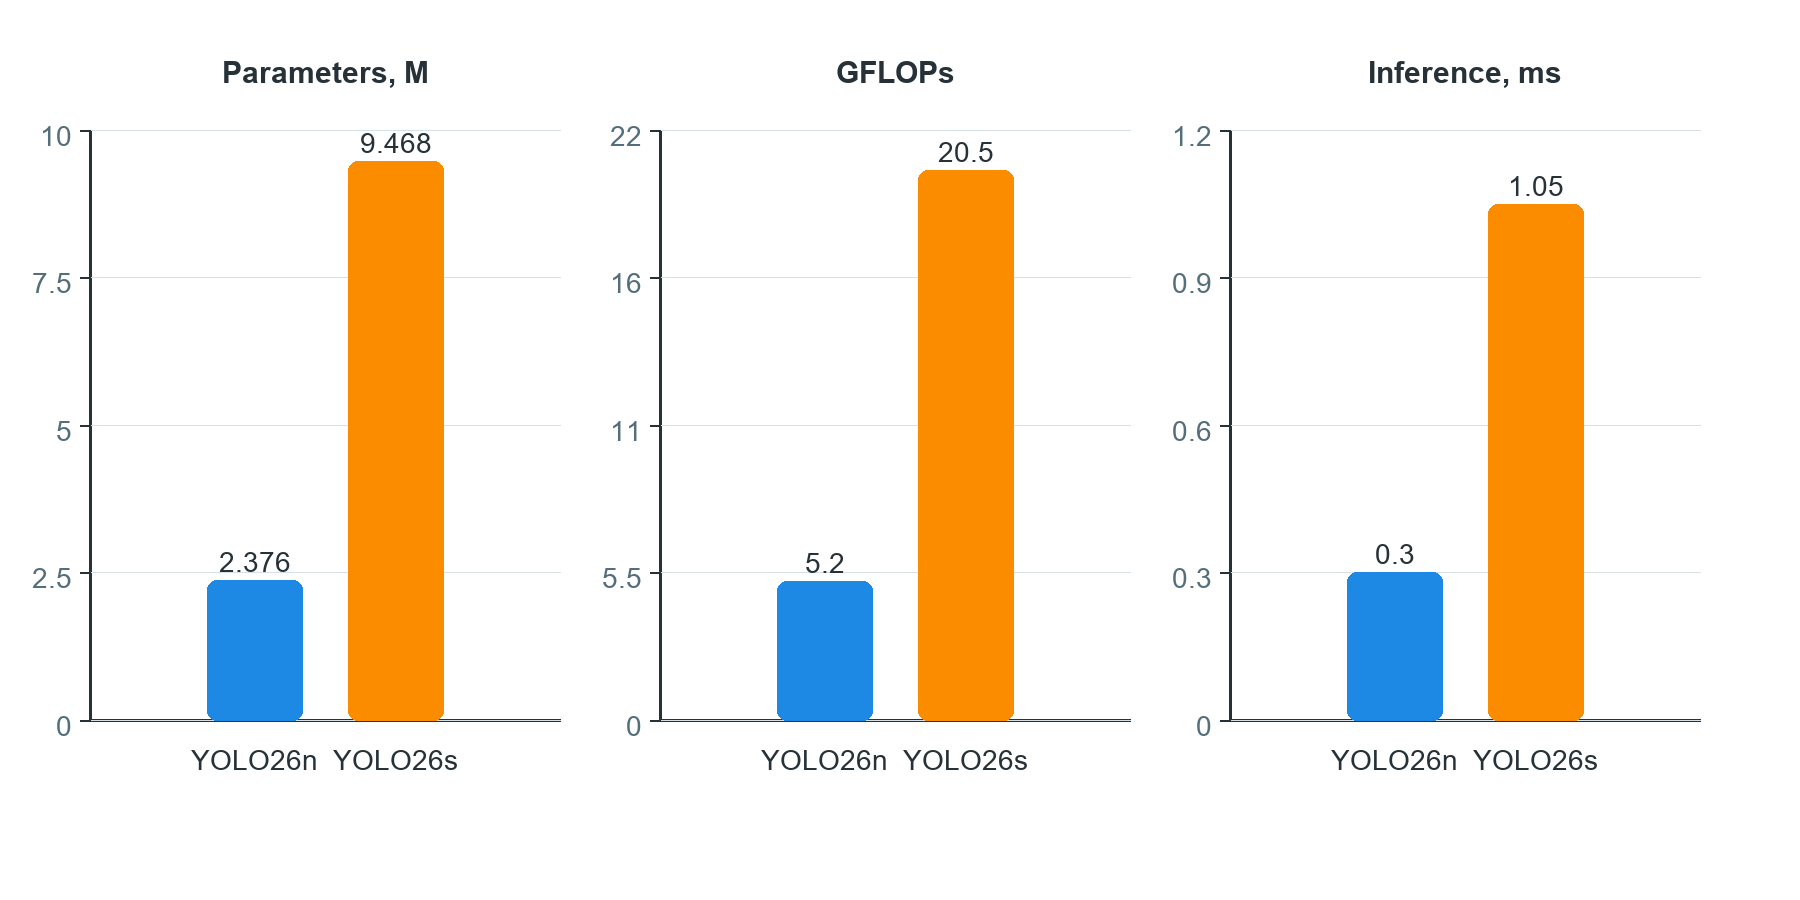
\includegraphics[width=0.86\linewidth]{ch05-yolo-results/fig12_model_cost.png}
\caption{Сравнение параметров и GFLOPs для YOLO26n и YOLO26s.}
\label{fig:model_cost}
\end{figure}

\section{Матрица ошибок}
Нормализованная матрица ошибок показывает, что на диагонали модель имеет сильные значения: $0.92$ для \texttt{top\_sleeved}, $0.95$ для \texttt{trousers}, $0.90$ для \texttt{shorts} и $0.87$ для \texttt{dress}. Более низкие значения у \texttt{top\_sleeveless} ($0.80$) и \texttt{outerwear} ($0.83$) объясняются визуальной близостью классов и дисбалансом данных. Заметная часть ошибок связана не с заменой одного класса одежды другим, а с фоном: для \texttt{top\_sleeved}, \texttt{dress}, \texttt{trousers} и \texttt{skirt} в background-столбце видны значения $0.36$, $0.15$, $0.14$ и $0.12$ соответственно. Для ROI-задачи это означает, что часть одежды может не получить textured ROI, если пороги и area policy выбраны слишком агрессивно.

\begin{figure}[H]
\centering
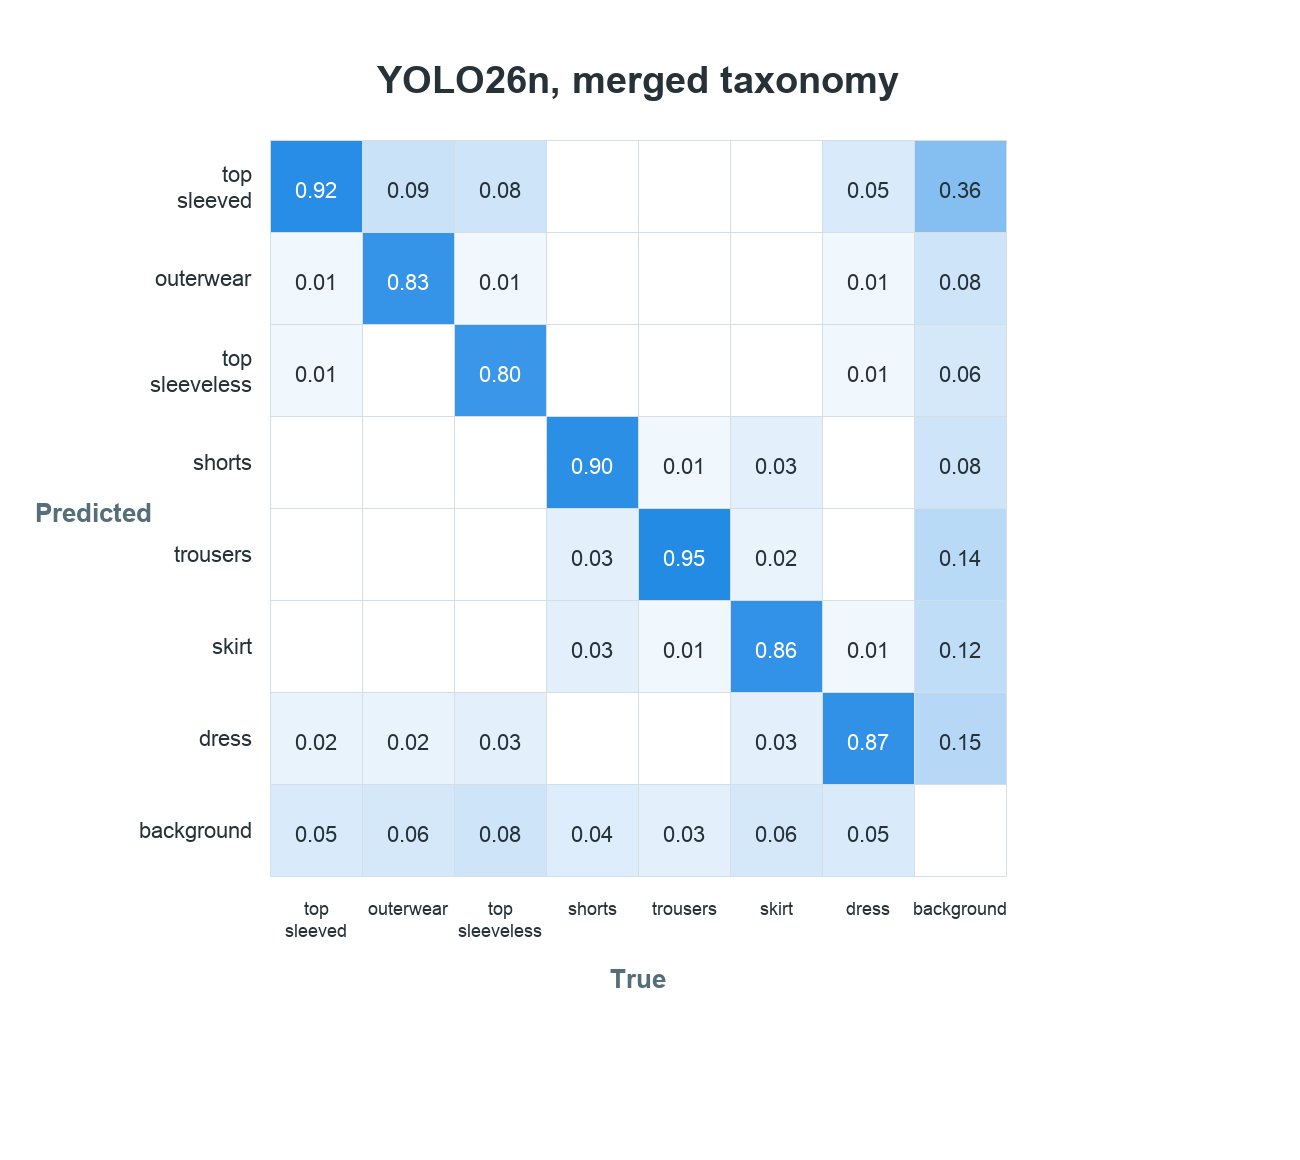
\includegraphics[width=0.86\linewidth]{ch05-yolo-results/fig13_confusion_matrix_norm.png}
\caption{Нормализованная матрица ошибок YOLO26n на объединенной 7-классовой таксономии.}
\label{fig:confusion}
\end{figure}

\begin{figure}[H]
\centering
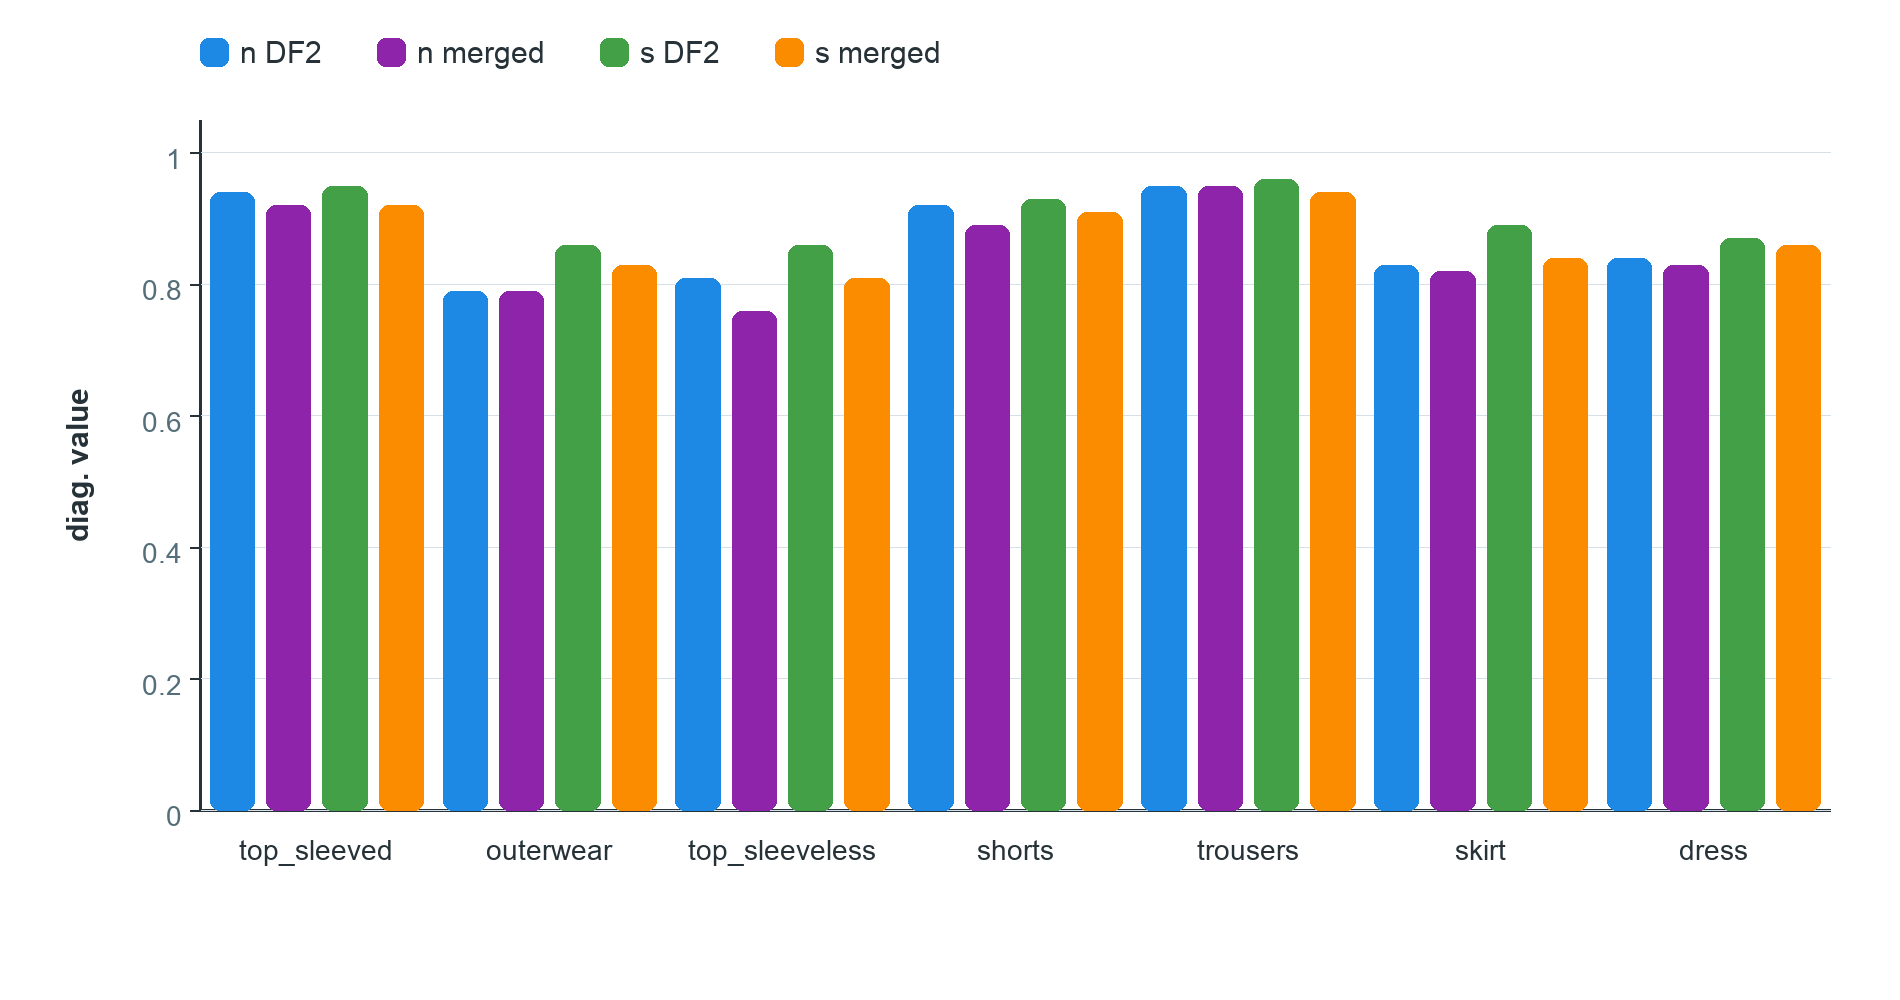
\includegraphics[width=0.92\linewidth]{ch05-yolo-results/fig13b_confusion_diag_compare.png}
\caption{Сравнение диагональных значений нормализованных матриц ошибок для четырех YOLO-экспериментов.}
\label{fig:confusion_diag_compare}
\end{figure}

Для задачи ROI proposal generation часть ошибок между близкими классами одежды менее критична, чем полный пропуск области: если модель все равно выделяет область одежды, она может быть защищена кодировщиком как textured ROI. Поэтому для интеграции в IDet важны не только class-level ошибки, но и геометрическое покрытие ROI относительно reference-разметки. Полные нормализованные матрицы для остальных запусков вынесены в приложение, чтобы не перегружать основной текст повторяющимися тепловыми картами.

\section{Почему выбран YOLO26n}
Финальное инженерное решение --- выбрать YOLO26n, а не YOLO26s. YOLO26s имеет более высокую точность на части экспериментов, но требует около 20.5 GFLOPs против 5.2 GFLOPs у YOLO26n. Цель ВКР --- не построить максимально точный fashion classifier, а получить модель, которую реалистично встроить в CPU-first IDet и затем проверить в режиме с ограниченным бюджетом на весь pre/post-processing. Поэтому YOLO26n является более обоснованным кандидатом для практической интеграции: он сохраняет mAP@0.5:0.95 = 0.818 на объединенном наборе и уменьшает вычислительную стоимость относительно YOLO26s примерно в четыре раза.

\begin{figure}[H]
\centering
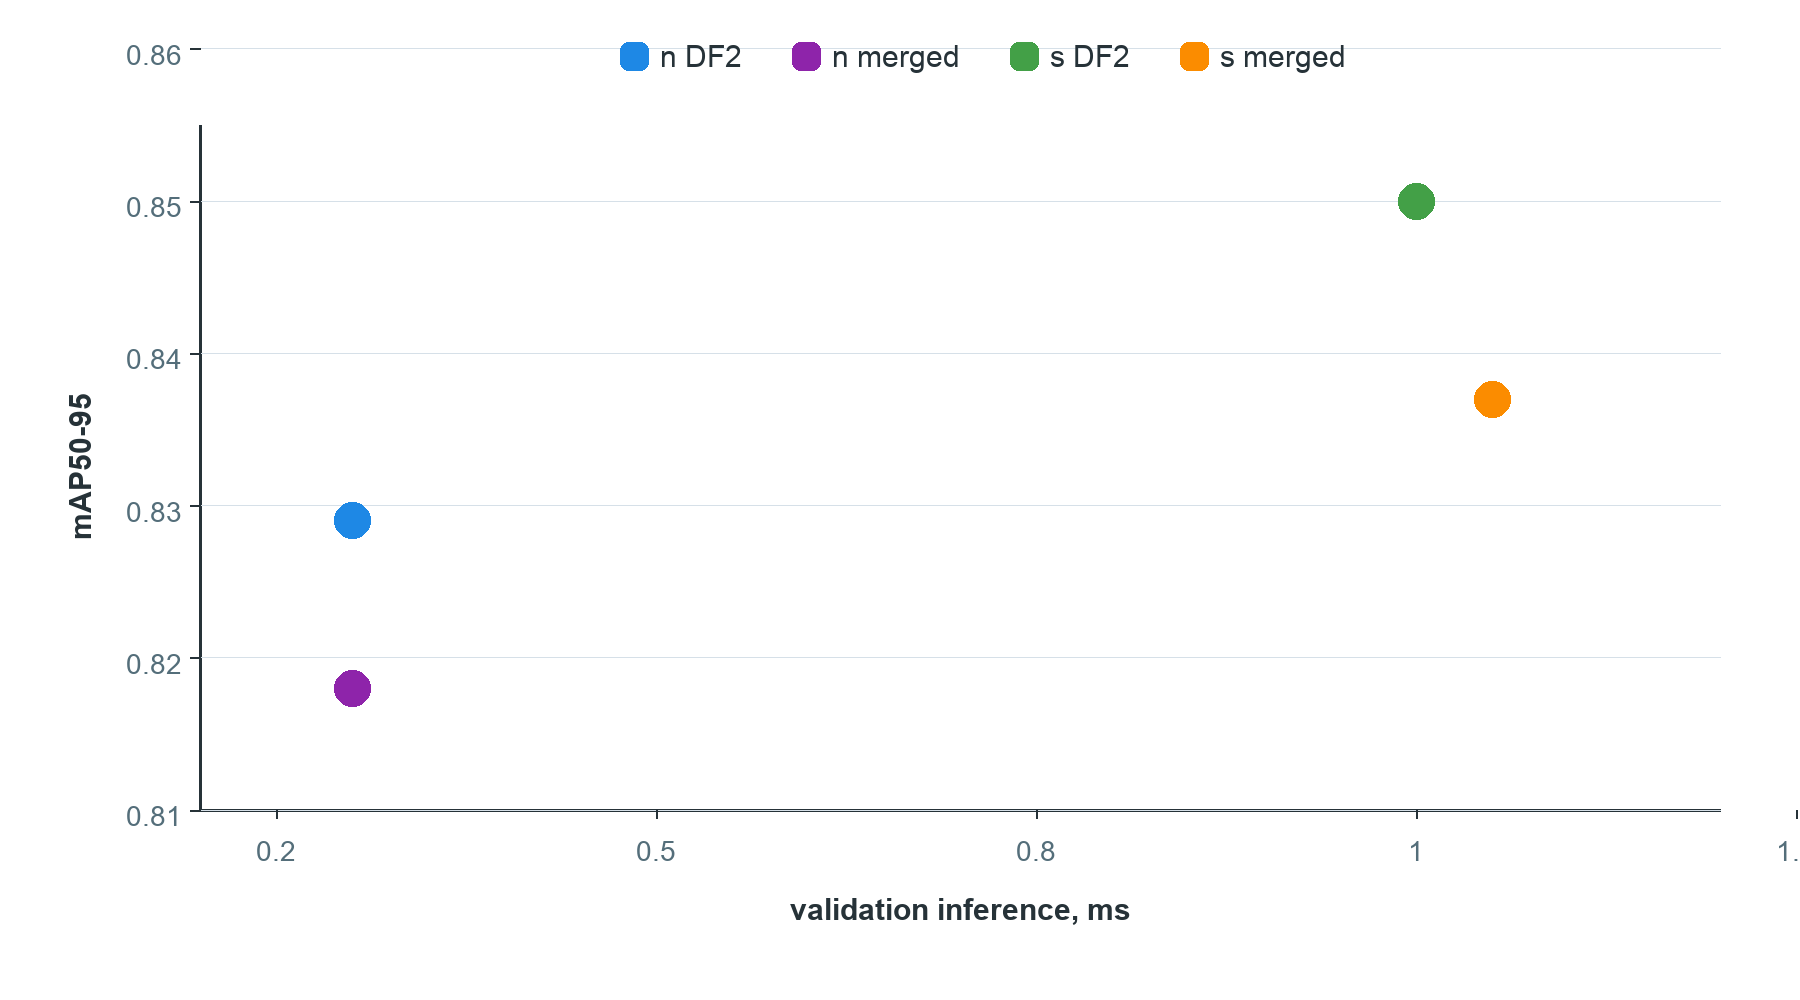
\includegraphics[width=0.82\linewidth]{ch05-yolo-results/fig14_quality_latency_tradeoff.png}
\caption{Компромисс между качеством детектора и вычислительной стоимостью по валидационным отчетам.}
\label{fig:quality_latency}
\end{figure}

\chapter{Интеграция ROI в видеокодирование}
\section{ROI как управляющий сигнал, а не конечный результат}
В данной работе ROI-детектор не является финальным продуктом сам по себе. Его выход --- это управляющий сигнал для кодировщика. Поэтому оценивать систему нужно не только по detection metrics, но и по тому, как ROI влияет на итоговое качество видео при фиксированном битрейте.

Пусть $S$ --- стратегия кодирования, $D$ --- ROI detector, $E$ --- encoder. Тогда полный конвейер можно записать как
\begin{equation}
\hat{V} = E(V, S(D(V))),
\label{eq:pipeline}
\end{equation}
где $V$ --- исходное видео, $D(V)$ --- последовательность ROI, $S$ --- политика приоритизации и mapping в qoffset, $\hat{V}$ --- сжатый поток. Важно, что $D$ не оптимизируется изолированно; он должен быть полезен внутри $E$.

\section{Политика qoffset}
Для каждой ROI задается приоритет $p_i$. Сильнее всего защищается текст, затем лица, затем textured ROI. Практическая политика может быть задана таблицей~\ref{tab:qoffset_policy}.

\begin{table}[H]
\centering
\caption{Пример политики приоритизации ROI}
\label{tab:qoffset_policy}
\begin{tabularx}{\linewidth}{lrrY}
\toprule
Тип ROI & Priority & qoffset & Причина \\
\midrule
Text ROI & 1.00 & -0.20 & Читаемость текста критична для пользователя. \\
Face ROI & 0.85 & -0.15 & Искажения лица заметны субъективно. \\
Textured ROI & 0.55 & -0.08 & Фактура повышает perceived sharpness, но не должна вытеснять текст/лицо. \\
Background & 0.00 & 0.00 & Фон кодируется без дополнительной защиты. \\
\bottomrule
\end{tabularx}
\end{table}

Эти значения не являются универсальными константами; они задают начальную инженерную политику для экспериментов. В реальной системе qoffset следует подбирать на validation corpus с учетом битрейта, кодека и контента.

\section{Fallback-режимы}
Поддержка ROI metadata различается между кодировщиками и сборками FFmpeg/x265 \cite{ffmpeg_roi,x265}. Поэтому в работе предусматриваются fallback-режимы:
\begin{enumerate}[label=\arabic*)]
  \item использование native ROI metadata, если кодировщик поддерживает \texttt{AVRegionOfInterest};
  \item настройка adaptive quantization и rate-control параметров;
  \item слабая предобработка фона вне ROI для снижения его локальной сложности;
  \item offline selection режим, где ROI используется только для анализа качества и построения отчетов.
\end{enumerate}

\section{Целевой эксперимент качества}
Финальная проверка должна сравнивать не только detection metrics, но и качество закодированного видео. Минимальная матрица экспериментов приведена в таблице~\ref{tab:quality_experiments}.

\begin{table}[H]
\centering
\caption{Матрица экспериментов ROI-aware кодирования}
\label{tab:quality_experiments}
\scriptsize
\begin{tabularx}{\linewidth}{lcccY}
\toprule
Конфигурация & Text & Face & Texture & Ожидаемый эффект \\
\midrule
Baseline & нет & нет & нет & Равномерное кодирование без пространственного приоритета. \\
Text-only & да & нет & нет & Рост читаемости текста и интерфейса. \\
Face-only & нет & да & нет & Улучшение качества лиц. \\
Text+Face & да & да & нет & Базовый semantic ROI режим. \\
Full ROI & да & да & да & Защита текста, лиц и фактурированных областей. \\
\bottomrule
\end{tabularx}
\end{table}

Измеряться должны VMAF, SSIM, ROI-weighted SSIM/VMAF, bitrate deviation, latency, FPS и стабильность ROI. Такой протокол связывает научную часть с практическим продуктом.


\chapter{Методика сравнения baseline и ROI-aware закодированного потока}
\section{Цель эксперимента}
Финальная проверка IDet должна выходить за пределы детекционных и inference-метрик. Цель эксперимента состоит в том, чтобы сравнить обычный закодированный поток без ROI и поток, закодированный с учетом ROI, полученных IDet. Сравнение должно выполняться при одинаковом исходном видео, одинаковом кодировщике, одинаковом preset, одинаковом целевом битрейте и одинаковых ограничениях на задержку. В такой постановке различие в качестве можно связывать именно с ROI-aware политикой, а не с изменением параметров кодирования.

Рабочая гипотеза состоит в том, что ROI-aware кодирование должно улучшить качество визуально значимых областей --- текста, лиц и фактурированных объектов --- за счет перераспределения битов от менее важных областей кадра. При этом глобальные VMAF/SSIM могут измениться умеренно, потому что ROI занимают лишь часть изображения. Поэтому основное подтверждение гипотезы следует искать в ROI-взвешенных метриках и визуальном сравнении локальных областей.

\section{Экспериментальные ветки}
Минимальная матрица эксперимента приведена в таблице~\ref{tab:roi_stream_variants}. Эта матрица задает фиксированные ветки сравнения и не содержит количественных выводов: численные метрики должны вноситься только после одинаковых прогонов кодировщика.

\begin{table}[H]
\centering
\caption{Ветки сравнения baseline и ROI-aware потока}
\label{tab:roi_stream_variants}
\small
\begin{tabularx}{\linewidth}{@{}p{0.18\linewidth}ccccY@{}}
\toprule
Ветка & Text & Face & Texture & ROI policy & Ожидаемый эффект \\
\midrule
Baseline & нет & нет & нет & ROI off & Равномерное кодирование без пространственного приоритета. \\
Text-only & да & нет & нет & text qoffset & Повышение читаемости текста, субтитров и интерфейса. \\
Face-only & нет & да & нет & face qoffset & Снижение заметных артефактов на лицах. \\
Text+Face & да & да & нет & semantic ROI & Базовая semantic ROI-политика для видео с человеком и текстом. \\
Full ROI & да & да & да & text+face+texture & Максимальная локальная защита при контроле площади ROI. \\
\bottomrule
\end{tabularx}
\end{table}

\section{Контроль переменных}
Для корректности эксперимента все ветки должны отличаться только ROI-политикой. Необходимо зафиксировать: исходный ролик, разрешение, fps, codec, preset, GOP structure, pixel format, target bitrate или CRF policy, версию FFmpeg/x265, параметры rate-control и способ расчета метрик. Если одновременно меняются ROI и preset кодировщика, вывод о полезности ROI становится некорректным.

\begin{table}[H]
\centering
\caption{Контролируемые параметры эксперимента кодирования}
\label{tab:encoding_control_variables}
\small
\begin{tabularx}{\linewidth}{@{}p{0.27\linewidth}Y@{}}
\toprule
Параметр & Требование \\
\midrule
Исходное видео & Один и тот же lossless или high-quality reference для всех веток. \\
Кодировщик & Одна и та же версия FFmpeg/x265 или другого backend. \\
Битрейт/CRF & Фиксированная политика rate-control; отклонение битрейта фиксируется отдельно. \\
Preset/GOP & Не изменяются между baseline и ROI-aware ветками. \\
ROI policy & Единственный изменяемый фактор эксперимента. \\
Метрики & VMAF, SSIM, ROI-weighted VMAF/SSIM, bitrate deviation, IDet latency. \\
Повторы & Для нестабильных окружений требуется несколько прогонов или фиксация CPU affinity/NUMA state. \\
\bottomrule
\end{tabularx}
\end{table}

\section{ROI-взвешенные метрики качества}
Глобальная метрика может слабо реагировать на локальное улучшение в ROI. Поэтому для анализа нужно дополнительно считать ROI-взвешенную версию метрики. Пусть $q_t(j)$ --- значение локальной метрики качества на блоке $j$ кадра $t$, а $w_t(j)$ --- вес блока. Тогда ROI-взвешенное качество может быть рассчитано как
\begin{equation}
Q_{\mathrm{ROI},t} =
\frac{\sum_{j=1}^{M_t} w_t(j) q_t(j)}{\sum_{j=1}^{M_t} w_t(j)}.
\label{eq:roi_weighted_metric}
\end{equation}
Вес можно задать через пересечение блока с ROI:
\begin{equation}
w_t(j) =
1 + \beta_{\mathrm{text}} I_{\mathrm{text}}(j)
  + \beta_{\mathrm{face}} I_{\mathrm{face}}(j)
  + \beta_{\mathrm{texture}} I_{\mathrm{texture}}(j),
\label{eq:roi_weight}
\end{equation}
где $I_{kind}(j)$ показывает, пересекается ли блок с ROI соответствующего типа. Значения $\beta$ должны фиксироваться в протоколе эксперимента. Для текстовых областей вес обычно должен быть выше, чем для textured ROI, поскольку потеря читаемости текста является более критичной.

\section{Форма фиксации итоговых метрик}
Таблица~\ref{tab:video_quality_template} задает форму фиксации результатов будущей серии кодирования. Прочерк означает, что метрика не публикуется до завершения одинаковых прогонов всех веток; такие поля не должны интерпретироваться как нулевые значения или предварительные результаты.

\begin{landscape}
\begin{table}[H]
\centering
\caption{Форма сравнения качества baseline и ROI-aware потока}
\label{tab:video_quality_template}
\scriptsize
\begin{tabularx}{\linewidth}{@{}p{0.14\linewidth}rrrrrrrrY@{}}
\toprule
Режим & Bitrate dev. & VMAF & ROI-VMAF & SSIM & ROI-SSIM & IDet p99 & Encoder FPS & E2E FPS & Интерпретация \\
\midrule
Baseline & --- & --- & --- & --- & --- & 0 & --- & --- & Равномерное кодирование без ROI. \\
Text-only & --- & --- & --- & --- & --- & --- & --- & --- & Ожидается рост читаемости текста. \\
Face-only & --- & --- & --- & --- & --- & --- & --- & --- & Ожидается улучшение лиц при умеренной площади ROI. \\
Text+Face & --- & --- & --- & --- & --- & --- & --- & --- & Ожидается лучший semantic ROI баланс для типового streaming-контента. \\
Full ROI & --- & --- & --- & --- & --- & --- & --- & --- & Ожидается максимальное локальное качество при контроле extra area. \\
\bottomrule
\end{tabularx}
\end{table}
\end{landscape}

\section{Критерии подтверждения гипотезы}
Гипотеза о пользе ROI-aware кодирования считается подтвержденной, если при фиксированном битрейте выполняются следующие условия:
\begin{enumerate}[label=\arabic*)]
  \item ROI-weighted VMAF или ROI-weighted SSIM выше, чем у baseline;
  \item bitrate deviation находится в допустимом диапазоне;
  \item p99 latency IDet не нарушает целевой бюджет видеоконвейера;
  \item визуальное сравнение ROI-кропов подтверждает улучшение текста, лиц или фактур;
  \item extra area ROI не становится настолько большой, что система фактически защищает весь кадр.
\end{enumerate}

Отрицательный или частично отрицательный результат также должен быть описан честно. Например, если ROI-aware режим увеличивает ROI-SSIM, но слишком сильно ухудшает фон или снижает FPS кодировщика, это означает необходимость более строгой area policy, другого qoffset mapping или temporal smoothing. На основании принципа ROI-aware распределения качества ожидается, что при фиксированном битрейте поток с ROI из IDet будет демонстрировать более высокое качество в визуально значимых областях по сравнению с равномерным кодированием. Основной ожидаемый эффект должен проявиться в ROI-взвешенных метриках, поскольку именно они учитывают локальное качество текста, лиц и фактурированных областей.

\chapter{Экспериментальная методика и критерии качества}
На рисунке~\ref{fig:experiment_protocol} показан общий протокол оценки: все режимы сравниваются на одинаковых входных видео, при одинаковом битрейте и одинаковых настройках кодировщика; меняется только ROI-политика. Такой протокол нужен, чтобы не спутать эффект ROI с эффектом другого пресета кодирования.

\begin{figure}[htbp]
\centering
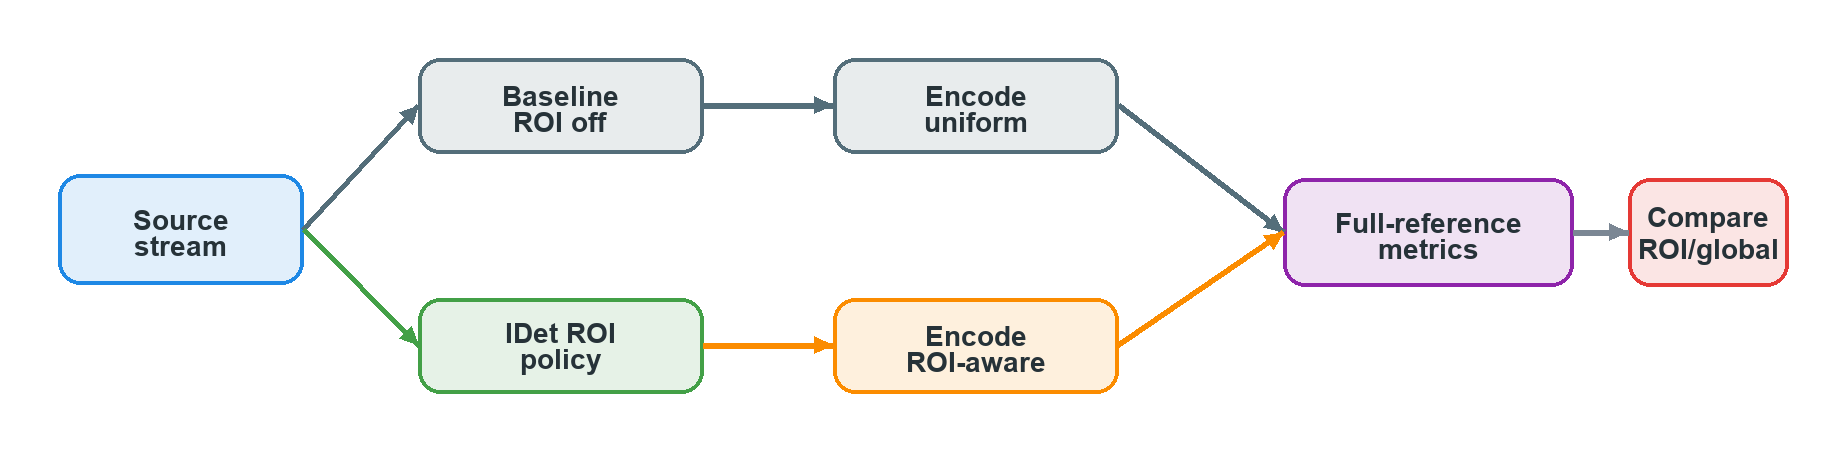
\includegraphics[width=0.96\linewidth]{ch09-video-quality/fig16_experiment_protocol.png}
\caption{Экспериментальный протокол оценки ROI-aware кодирования.}
\label{fig:experiment_protocol}
\end{figure}

\section{Метрики качества видео}
SSIM оценивает структурное сходство изображений и является классической full-reference метрикой \cite{ssim}. В упрощенном виде SSIM для двух окон $x$ и $y$ записывается как
\begin{equation}
SSIM(x,y)=\frac{(2\mu_x\mu_y+C_1)(2\sigma_{xy}+C_2)}{(\mu_x^2+\mu_y^2+C_1)(\sigma_x^2+\sigma_y^2+C_2)}.
\label{eq:ssim}
\end{equation}
VMAF объединяет несколько признаков качества и лучше согласуется с субъективным восприятием в ряде видеосценариев \cite{vmaf}. В данной работе VMAF рассматривается как основная глобальная метрика, а ROI-weighted SSIM/VMAF --- как дополнительная метрика для анализа локального улучшения.

\section{Системные метрики}
Так как цель работы --- не только качество, но и deployability, обязательны системные метрики:
\begin{enumerate}[label=\arabic*)]
  \item latency pre-processing;
  \item latency inference;
  \item latency post-processing;
  \item суммарная задержка кадра;
  \item p50/p90/p95/p99;
  \item memory footprint;
  \item FPS;
  \item CPU utilization.
\end{enumerate}

Инженерная целевая точка для IDet --- $\leq 10\,\ms$ на кадр для всего ROI pipeline. Это соответствует примерно 100 FPS и оставляет некоторый бюджет для кодировщика и системной обвязки. Достижение этой точки должно проверяться отдельным benchmark-прогоном, а не выводиться из метрик обучения YOLO-модели.

\section{Метрики покрытия ROI}
Для оценки качества ROI в практическом pipeline недостаточно считать только число найденных областей. Конфигурация может вернуть много box-кандидатов, но при этом пропустить часть reference ROI или чрезмерно расширить защищаемую область. Поэтому для сравнения режимов IDet используется геометрическая оценка покрытия относительно reference-прогона. Reference boxes в этой постановке не являются ground truth-разметкой; это инженерный proxy, полученный более дорогой или более консервативной конфигурацией.

Пусть $R_{\mathrm{ref}}$ --- объединение reference ROI, $R_{\mathrm{cand}}$ --- объединение candidate ROI, а $S(\cdot)$ --- площадь множества пикселей. Тогда используются метрики:
\begin{equation}
\operatorname{AreaRecall} =
\frac{S(R_{\mathrm{ref}}\cap R_{\mathrm{cand}})}
{S(R_{\mathrm{ref}})}, \qquad
\operatorname{AreaPrecision} =
\frac{S(R_{\mathrm{ref}}\cap R_{\mathrm{cand}})}
{S(R_{\mathrm{cand}})},
\label{eq:area_recall_precision}
\end{equation}
\begin{equation}
\operatorname{AreaF_1} =
2 \cdot
\frac{\operatorname{AreaRecall}\cdot \operatorname{AreaPrecision}}
{\operatorname{AreaRecall}+\operatorname{AreaPrecision}},
\label{eq:area_f1}
\end{equation}
\begin{equation}
\operatorname{ExtraAreaRatio} =
\frac{S(R_{\mathrm{cand}})-S(R_{\mathrm{ref}}\cap R_{\mathrm{cand}})}
{S(R_{\mathrm{ref}})}.
\label{eq:extra_area_ratio}
\end{equation}

Метрика $\operatorname{AreaRecall}$ показывает, какая доля эталонной ROI-площади покрыта кандидатом, $\operatorname{AreaPrecision}$ штрафует за раздутые ROI, $\operatorname{AreaF_1}$ балансирует покрытие и аккуратность, а $\operatorname{ExtraAreaRatio}$ ограничивает лишнюю защищаемую площадь. В финальных таблицах performance-quality конфигурации должны сортироваться по $p99$ latency по возрастанию, а качество должно проверяться по ограничениям на эти area-based метрики.

\section{Дисциплина CPU-only benchmark}
Для измерения IDet на CPU главным источником latency должны быть значения, которые печатает сам \texttt{idet\_app}: \texttt{p50\_ms}, \texttt{p90\_ms}, \texttt{p95\_ms} и \texttt{p99\_ms}. Время внешнего Python \texttt{subprocess} допустимо сохранять только как служебное поле, но не как latency модели или pipeline. Для чистого benchmark необходимо отключать отрисовку, dump и подробный вывод: \texttt{--is\_draw 0 --is\_dump 0 --verbose 0}.

Финальные performance-выводы должны строиться только на release/perf-сборке без ASan/UBSan, поскольку санитайзеры меняют профиль памяти, futex/wait и распределение задержек. Для ARM/Kunpeng-прогонов дополнительно фиксируются число доступных CPU, NUMA-политика, параметры \texttt{threads\_intra}, \texttt{threads\_inter}, \texttt{tile\_omp}, режим \texttt{cpu\_placement}, memory binding и состояние automatic NUMA balancing. Если эти условия не зафиксированы, вывод о p99 latency следует считать ограниченным данным окружением.


\section{NUMA, Kunpeng и ONNX Runtime CPU Execution Provider}
Целевое CPU-only окружение требует отдельной дисциплины измерений. На серверных ARM-системах, таких как Kunpeng 920, итоговая задержка зависит не только от числа потоков, но и от размещения потоков по NUMA-узлам, локальности памяти и взаимодействия OpenMP с thread pool ONNX Runtime. ONNX Runtime предоставляет настройки intra-op и inter-op threads, а также рекомендации по настройке производительности и threading \cite{ort_tuning,ort_threading}. Поэтому параметры \texttt{threads\_intra}, \texttt{threads\_inter} и \texttt{tile\_omp} должны быть частью экспериментальной таблицы, а не скрытой настройкой окружения.

Automatic NUMA balancing в Linux может быть полезен для обычных приложений, но в pinned benchmark он способен добавлять шум за счет page-fault based migration и сканирования памяти \cite{linux_numa_balancing}. Поэтому состояние \texttt{kernel.numa\_balancing} необходимо фиксировать в протоколе. Если benchmark выполняется на ограниченном cpuset, например только на CPU 48--57, то сравнение конфигураций справедливо именно для этого cpuset. Изменение числа доступных CPU требует повторного grid search, поскольку оптимальные \texttt{threads\_intra} и \texttt{tile\_omp} могут измениться.

Для углубленного анализа hotspot-ов допустимо использовать CCA/perf profiling. Linux perf предоставляет механизм sampling и hardware performance counters \cite{linux_perf}. На ARM-системах также может использоваться Statistical Profiling Extension, если она доступна ядру и firmware \cite{arm_spe}. Если профилировщик выводит предупреждение о недоступности SPE, это не является ошибкой IDet, но ограничивает глубину анализа микроархитектурных событий.

\begin{table}[H]
\centering
\caption{Минимальный протокол CPU-only performance-прогона}
\label{tab:cpu_benchmark_protocol}
\small
\begin{tabularx}{\linewidth}{@{}p{0.28\linewidth}Y@{}}
\toprule
Параметр & Что фиксировать \\
\midrule
Build profile & \texttt{gcc-perf}/\texttt{clang-perf}, отсутствие ASan/UBSan. \\
CPU topology & Модель CPU, число физических/логических ядер, доступный cpuset. \\
NUMA state & NUMA node, memory locality, состояние \texttt{kernel.numa\_balancing}. \\
ORT settings & \texttt{threads\_intra}, \texttt{threads\_inter}, graph optimization level, I/O Binding. \\
Tiling settings & \texttt{tiles\_rc}, \texttt{tile\_overlap}, \texttt{tile\_omp}, fixed tile input. \\
Benchmark mode & \texttt{--is\_draw 0 --is\_dump 0 --verbose 0}. \\
Quality dump mode & \texttt{--is\_draw 0 --is\_dump 1 --verbose 0}. \\
Latency metrics & p50, p90, p95, p99 из stdout \texttt{idet\_app}. \\
Quality proxy & area recall, area precision, area F1, extra area ratio. \\
\bottomrule
\end{tabularx}
\end{table}

\section{Кривые качества и вычислительной стоимости}
Для каждой конфигурации можно построить quality-cost curve:
\begin{equation}
\mathcal{C}(S) = \left( L(S), Q_{\roi}(S), R(S) \right),
\label{eq:quality_cost}
\end{equation}
где $L$ --- задержка, $Q_{\roi}$ --- ROI-взвешенное качество, $R$ --- битрейт. Стратегия $S_1$ доминирует стратегию $S_2$, если
\begin{equation}
Q_{\roi}(S_1) \geq Q_{\roi}(S_2), \quad L(S_1) \leq L(S_2), \quad R(S_1) \leq R(S_2),
\label{eq:pareto}
\end{equation}
и хотя бы одно неравенство строгое. Такой Pareto-анализ позволяет не сводить работу к одной метрике.

\section{Абляционное исследование}
Для доказательства полезности каждого компонента нужен ablation study. В частности, следует сравнить:
\begin{enumerate}[label=\arabic*)]
  \item без ROI;
  \item только text ROI;
  \item только face ROI;
  \item только textured ROI;
  \item text + face;
  \item text + face + textured;
  \item разные пороги confidence для YOLO26n;
  \item разные ограничения $\alpha$ на площадь ROI;
  \item разные значения qoffset для textured ROI;
  \item native ROI metadata против fallback preprocessing.
\end{enumerate}

Такой протокол делает работу воспроизводимой и защищает ее от типичной слабости ML-проектов: наличия хорошей модели без понимания ее системного эффекта.

\chapter{Экспериментальное исследование производительности IDet}
\section{Состав benchmark-эксперимента}
Для оценки CPU-only поведения IDet использованы сводные таблицы grid-search эксперимента по трем режимам: text, face и textured ROI. Они содержат не только latency, но и area-based quality proxy относительно reference-прогона: $\operatorname{AreaRecall}$, $\operatorname{AreaPrecision}$, $\operatorname{AreaF_1}$ и $\operatorname{ExtraAreaRatio}$. Это принципиально важно: конфигурация не выбирается только по числу детекций или минимальному p50, потому что для кодировщика опасны как пропущенные ROI, так и чрезмерно раздутые области.

Во всех трех режимах чистый latency benchmark запускался с отключенными отрисовкой, сохранением диагностических областей и подробным выводом. Извлечение областей выполнялось отдельным коротким прогоном; эти режимы нельзя смешивать, иначе latency будет включать диагностическую запись результатов. В таблице~\ref{tab:bench_speed_quality} показаны две рабочие точки для каждого режима: speed-first и quality-balanced. Первая минимизирует p99 при выполнении базовых ограничений на coverage, вторая выбирает максимальный $\operatorname{AreaF_1}$ из сводной таблицы и показывает цену качества в миллисекундах.

\begin{landscape}
\begin{table}[H]
\centering
\caption{Рабочие точки IDet по результатам grid-search эксперимента}
\label{tab:bench_speed_quality}
\scriptsize
\begin{tabularx}{\linewidth}{@{}llrrrrrrrrlllrrrr@{}}
\toprule
Режим & Точка & p50 & p95 & p99 & Area Recall & Area Precision & Area F1 & Extra & Boxes & Tiles & Fixed HW & Threads & Intra & Inter & OMP & Desired \\
\midrule
Text & speed-first & 7.962 & 8.024 & 8.032 & 0.886 & 0.709 & 0.788 & 0.363 & 51 & 5x6 & 64x128 & 2/1/30 & 2 & 1 & 30 & 32 \\
Text & quality-balanced & 15.496 & 16.059 & 16.099 & 0.940 & 0.723 & 0.817 & 0.361 & 43 & 3x4 & 128x192 & 8/1/12 & 8 & 1 & 12 & 20 \\
Face & speed-first & 6.074 & 6.198 & 6.203 & 0.859 & 0.894 & 0.876 & 0.102 & 10 & 1x5 & 288x96 & 8/1/5 & 8 & 1 & 5 & 13 \\
Face & quality-balanced & 17.086 & 17.552 & 17.808 & 0.988 & 0.950 & 0.969 & 0.052 & 13 & 1x4 & 512x224 & 8/1/4 & 8 & 1 & 4 & 12 \\
Textured & speed-first & 9.018 & 9.163 & 9.230 & 0.920 & 0.827 & 0.871 & 0.192 & 37 & 2x4 & 128x128 & 8/1/8 & 8 & 1 & 8 & 16 \\
Textured & quality-balanced & 11.793 & 11.936 & 11.954 & 0.959 & 0.873 & 0.914 & 0.140 & 27 & 1x5 & 288x96 & 8/1/5 & 8 & 1 & 5 & 13 \\
\bottomrule
\end{tabularx}
\end{table}
\end{landscape}

\section{Latency-quality trade-off}
На рисунке~\ref{fig:bench_p99_area_f1} каждая точка соответствует одной конфигурации grid search. Для всех трех режимов виден ожидаемый компромисс: повышение качества покрытия обычно требует большего p99, однако форма компромисса различается. Text ROI имеет быстрые конфигурации около 8 мс p99, но максимальный $\operatorname{AreaF_1}$ достигается около 16 мс. Face ROI показывает самый быстрый режим около 5.4--6.2 мс p99, но quality-balanced конфигурации требуют уже 17--18 мс. Textured ROI оказывается наиболее удачным для текущего набора: speed-first точка уже дает $\operatorname{AreaF_1}=0.871$ при p99=9.230 мс.

\begin{figure}[H]
\centering
\includegraphics[width=0.90\linewidth]{ch07-performance/fig17_bench_p99_area_f1.png}
\caption{Компромисс между p99 latency и Area F1 для text, face и textured режимов IDet.}
\label{fig:bench_p99_area_f1}
\end{figure}

На рисунке~\ref{fig:bench_best_latency} отдельно показаны p50/p95/p99 для speed-first конфигураций, прошедших ограничения на area-quality. Разница между p50 и p99 в этих точках невелика: например, для textured ROI p50=9.018 мс, p95=9.163 мс и p99=9.230 мс. Это важно для видеоконвейера: стабильный хвост задержки полезнее, чем один хороший средний показатель при редких длинных выбросах.

\begin{figure}[H]
\centering
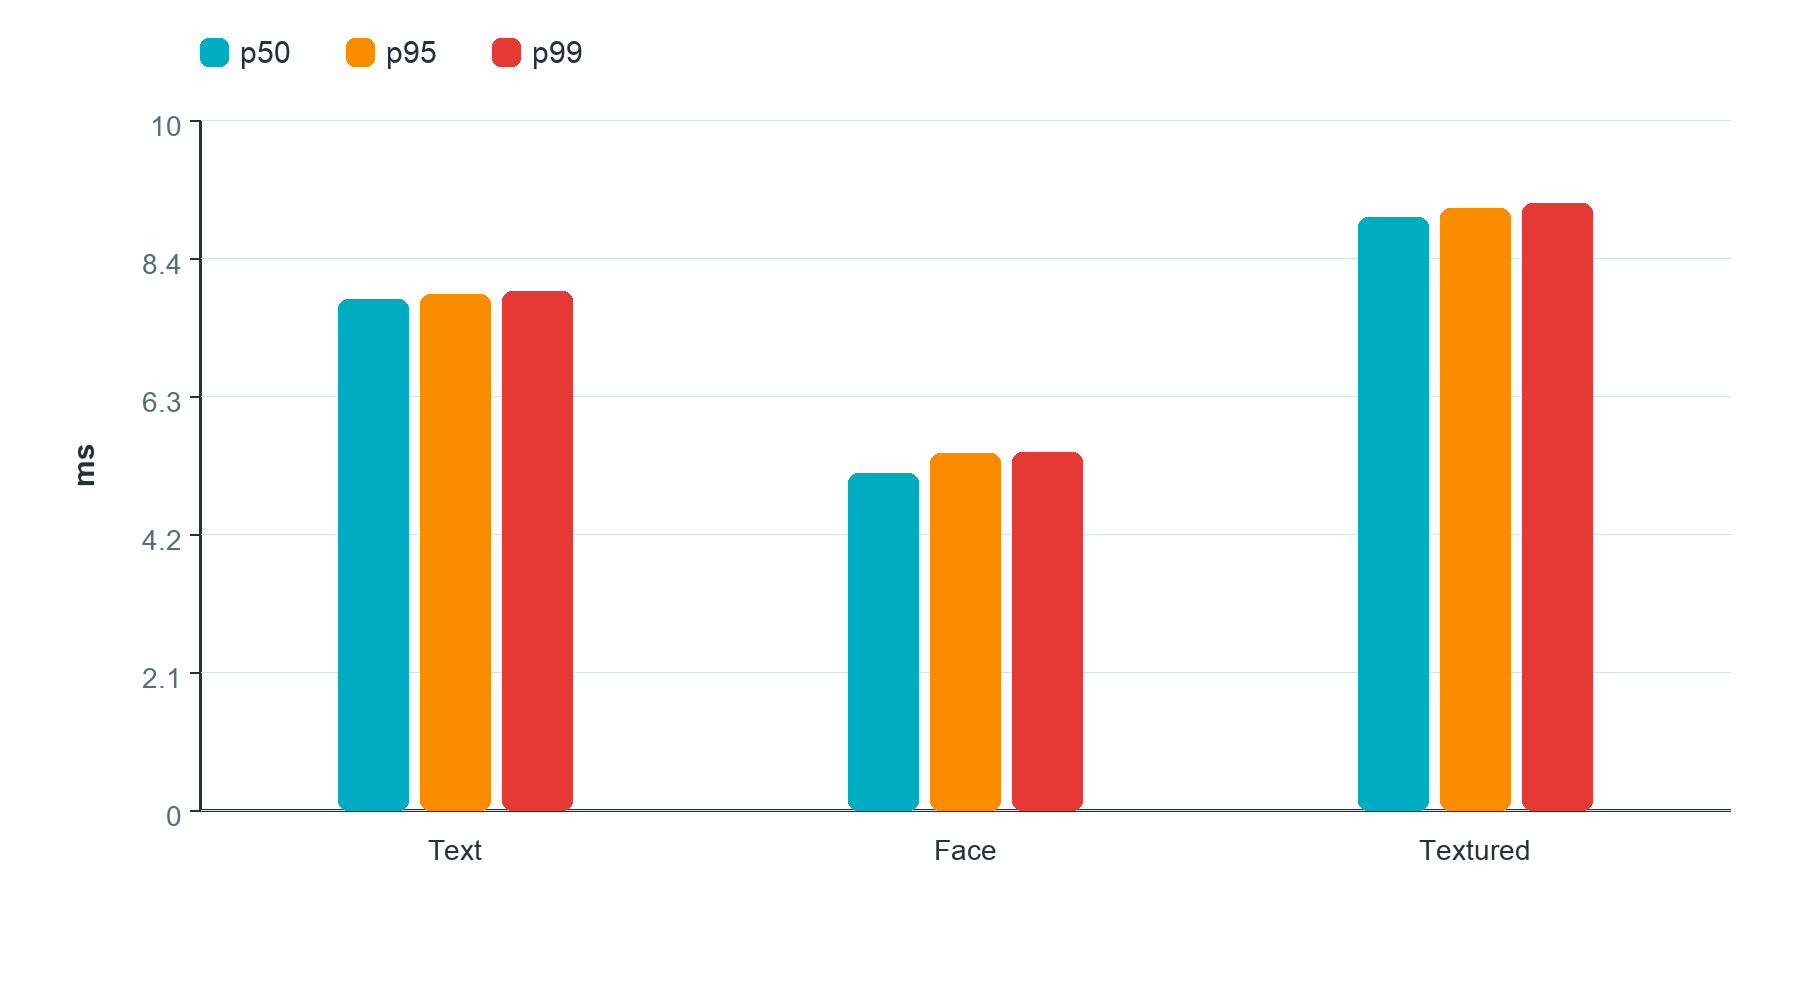
\includegraphics[width=0.86\linewidth]{ch07-performance/fig18_bench_best_latency.png}
\caption{p50/p95/p99 для выбранных speed-first конфигураций text, face и textured режимов.}
\label{fig:bench_best_latency}
\end{figure}

\section{Интерпретация по режимам}
Для text ROI наилучший быстрый вариант использует сетку 5x6, fixed input 64x128, \texttt{threads\_intra}=2 и \texttt{tile\_omp}=30. Он дает p99=8.032 мс и $\operatorname{AreaF_1}=0.788$. Более качественная точка повышает area recall до 0.940 и $\operatorname{AreaF_1}$ до 0.817, но p99 растет до 16.099 мс. Следовательно, text ROI имеет два практических режима: быстрый для жесткого latency budget и более дорогой для сценариев, где читаемость текста важнее хвоста задержки.

Для face ROI tiled-подход явно полезен в speed-first сценарии. В сводной таблице присутствуют single-shot точки для face; минимальный p99 single-shot составляет 14.008 мс при $\operatorname{AreaF_1}=0.939$, тогда как tiled speed-first дает p99=6.203 мс при $\operatorname{AreaF_1}=0.876$. Это показывает, что tiling снижает задержку, но может менять геометрию покрытия. Поэтому выбор face-конфигурации должен зависеть от того, что важнее в конкретном режиме: минимальный p99 или максимально точное покрытие лиц.

Для textured ROI лучшая быстрая точка уже удовлетворяет строгим требованиям качества: $\operatorname{AreaRecall}=0.920$, $\operatorname{AreaPrecision}=0.827$, $\operatorname{AreaF_1}=0.871$ и $\operatorname{ExtraAreaRatio}=0.192$. Quality-balanced точка улучшает $\operatorname{AreaF_1}$ до 0.914 и снижает лишнюю площадь до 0.140 при p99=11.954 мс. Для textured ROI это особенно важно, потому что чрезмерно широкие области одежды могут отнимать биты у текста и лица.

\section{Profiling и I/O Binding}
Профилирование использовалось как диагностический инструмент для выявления bottleneck, а не как источник финальных production latency. Сравнивались два режима: без I/O Binding и с I/O Binding при зафиксированном состоянии NUMA balancing. Результаты показывают, что I/O Binding существенно улучшает локальность памяти: доля \textit{inner} traffic растет с 41.01\% до 77.22\% для textured single, с 48.01\% до 94.31\% для textured tiled, с 55.49\% до 94.88\% для face tiled и с 48.73\% до 91.43\% для text tiled. Это подтверждает инженерный смысл binding: он не просто ускоряет отдельный вызов, а делает размещение памяти более предсказуемым в NUMA-сценарии.

\begin{table}[H]
\centering
\caption{Влияние I/O Binding на локальность памяти}
\label{tab:memory_locality}
\small
\begin{tabularx}{\linewidth}{lrrrrr}
\toprule
Режим & Inner with, \% & Inner without, \% & Прирост, п.п. & Total with, GB & Total without, GB \\
\midrule
Textured single & 77.22 & 41.01 & 36.21 & 15.82 & 35.75 \\
Textured tiled & 94.31 & 48.01 & 46.30 & 35.56 & 45.68 \\
Face single & 84.63 & 56.47 & 28.16 & 9.41 & 14.40 \\
Face tiled & 94.88 & 55.49 & 39.39 & 22.93 & 20.77 \\
Text single & 52.35 & 44.87 & 7.48 & 31.72 & 40.24 \\
Text tiled & 91.43 & 48.73 & 42.70 & 23.65 & 25.94 \\
\bottomrule
\end{tabularx}
\end{table}

\begin{figure}[H]
\centering
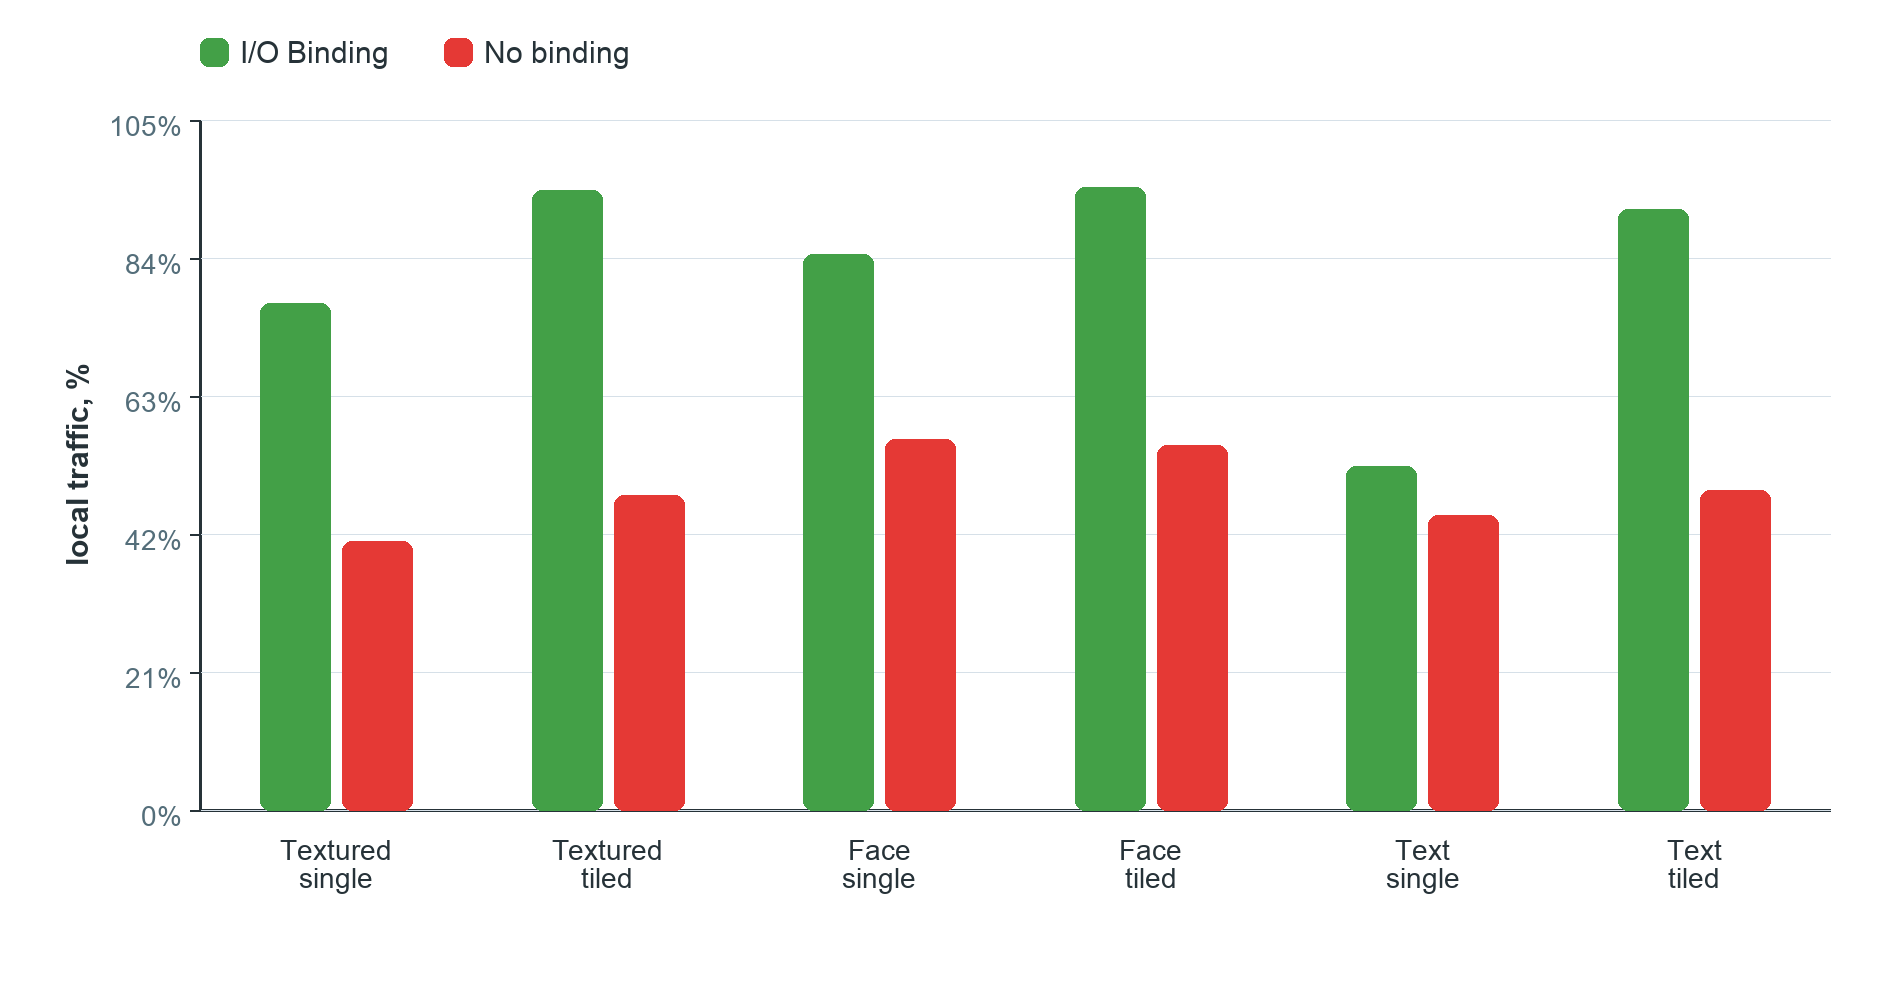
\includegraphics[width=0.90\linewidth]{ch08-profiling/fig19_memory_locality.png}
\caption{Доля локального memory traffic при включенном и выключенном I/O Binding.}
\label{fig:memory_locality}
\end{figure}

Интерпретировать profiling нужно аккуратно. В большинстве режимов total memory traffic с binding ниже, но для face tiled он увеличивается с 20.77 GB до 22.93 GB. Следовательно, корректный вывод состоит не в том, что binding всегда уменьшает общий объем трафика, а в том, что он радикально повышает локальность обращений. Для pinned CPU benchmark это важнее: локальные обращения уменьшают зависимость от межсокетного трафика и делают p95/p99 более управляемыми.

\section{Top-Down Microarchitecture Analysis}
Top-Down Microarchitecture Analysis классифицирует, как процессор расходует pipeline slots \cite{topdown,arm_topdown}. В этой модели \textit{Retiring} означает долю полезно завершенных инструкций, \textit{Frontend Bound} --- ограничения подачи инструкций, \textit{Backend Bound} --- ожидание данных, памяти или execution resources, а \textit{Bad Speculation} --- потери из-за неверных предсказаний и сбросов pipeline.

На рисунке~\ref{fig:tma_breakdown} показана реконструированная сводка по данным профилирования. Single-shot режимы имеют более высокую долю Retiring: примерно 60.65\% для text без binding, 62.77\% для face без binding и 65.88\% для textured без binding. В tiled-режиме доля Backend Bound возрастает: для text без binding --- до 51.94\%, для face без binding --- до 49.47\%, для textured без binding --- до 58.60\%. При включенном I/O Binding картина принципиально не меняется: tiled-режим textured ROI остается backend-bound с 60.63\% Backend Bound.

\begin{figure}[H]
\centering
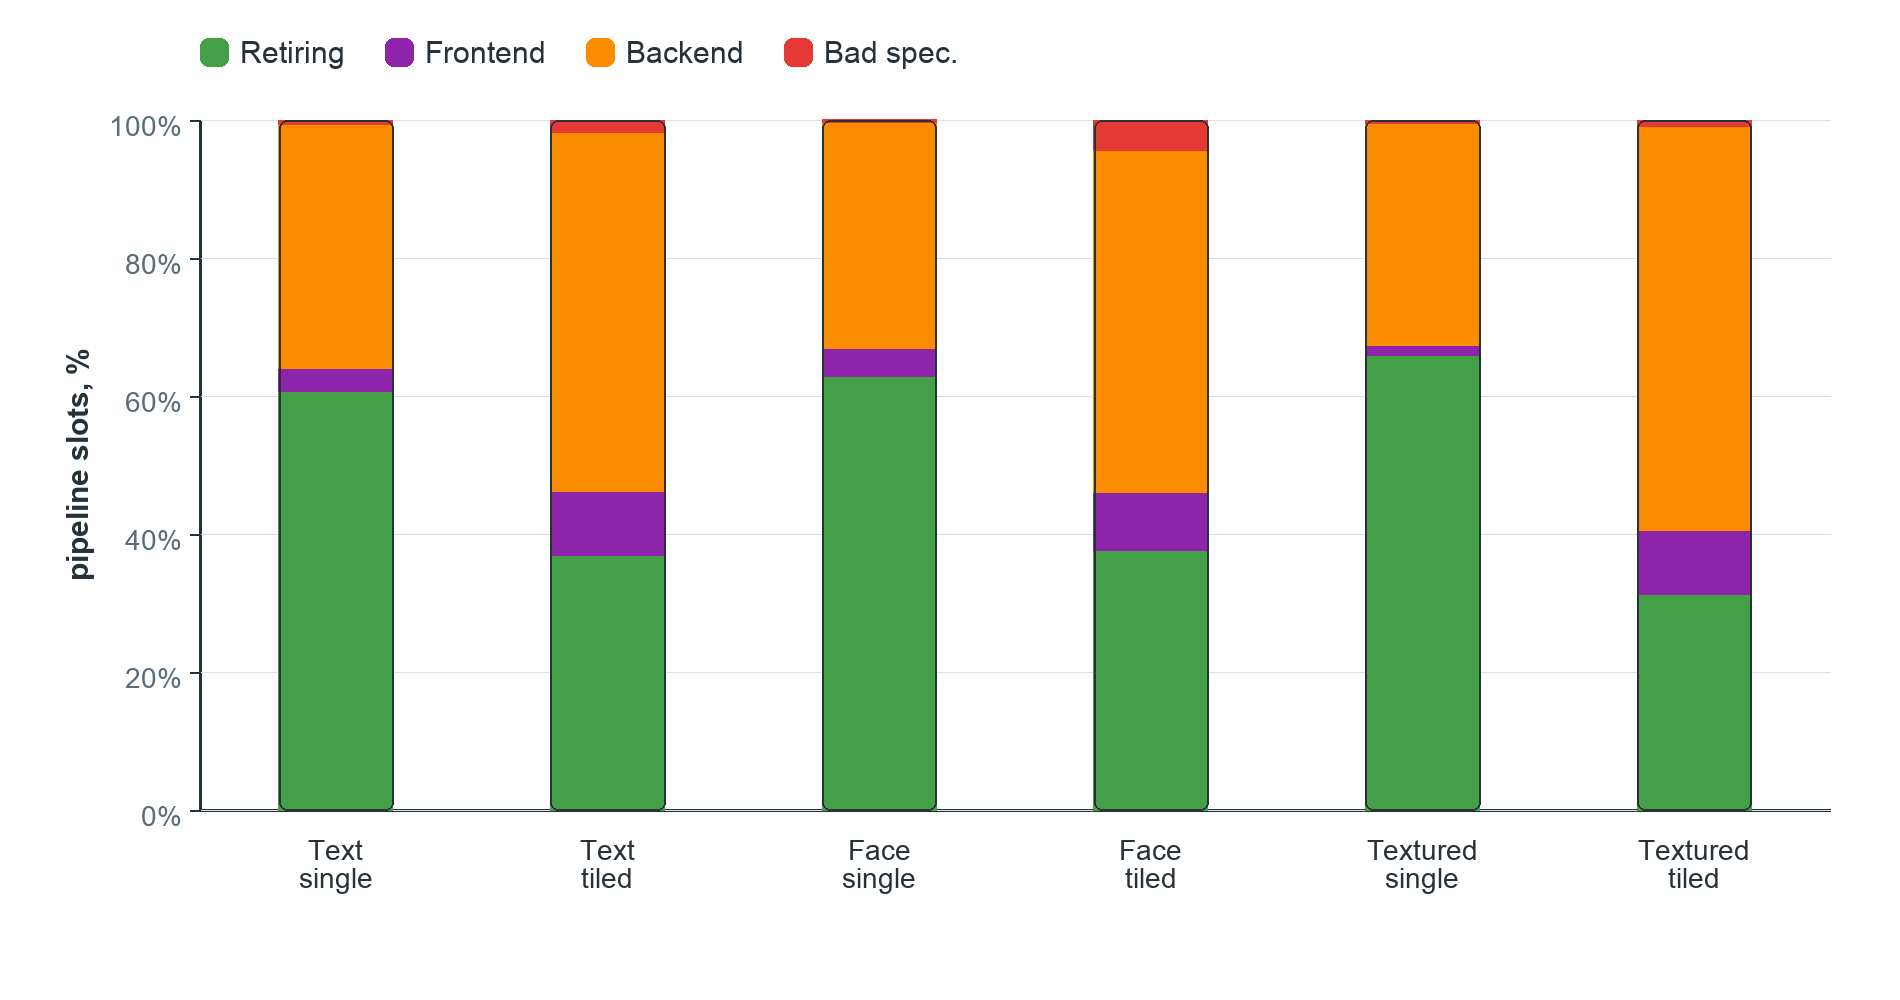
\includegraphics[width=0.95\linewidth]{ch08-profiling/fig20_tma_breakdown.png}
\caption{Top-Down Microarchitecture Analysis для single/tiled режимов с I/O Binding и без него.}
\label{fig:tma_breakdown}
\end{figure}

Отдельно важно, что tiled-режимы резко увеличивают долю NEON SIMD instructions: для text ROI примерно с 10--14\% до 40\%, для face ROI примерно с 9--14\% до 33--34\%, для textured ROI примерно с 6--8\% до 36--37\%. Это означает, что tiled execution лучше задействует векторные участки вычислений, но одновременно усиливает роль памяти, синхронизации и runtime scheduling. Поэтому выбор tiled-конфигурации должен оцениваться по p99 и area-quality одновременно, а не только по факту роста SIMD-доли.

\begin{figure}[H]
\centering
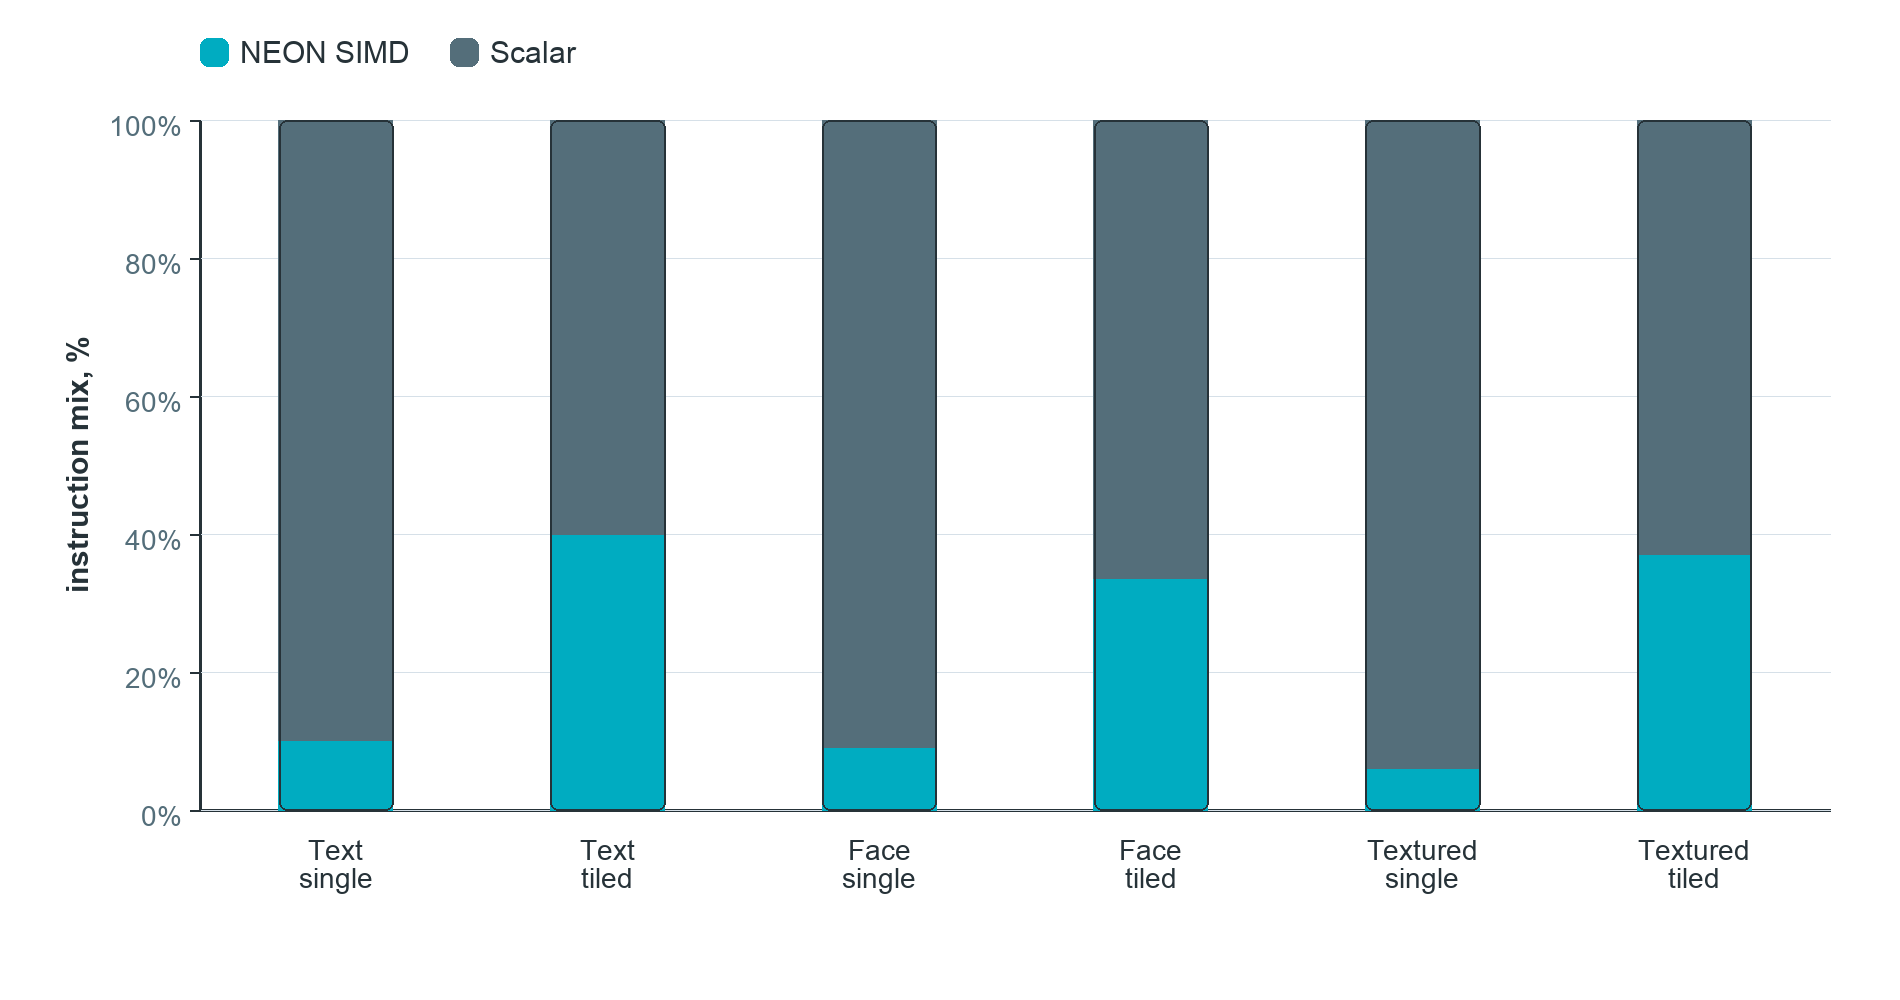
\includegraphics[width=0.82\linewidth]{ch08-profiling/fig21_neon_mix.png}
\caption{Доля NEON SIMD instructions в single и tiled режимах.}
\label{fig:neon_mix}
\end{figure}

\section{Ограничения текущих benchmark-данных}
Полученные benchmark-таблицы являются сильным экспериментальным основанием для выбора конфигураций IDet, но их нельзя отождествлять с финальным end-to-end качеством видеостриминга. Во-первых, area-based метрики сравнивают candidate boxes с reference-прогоном, а не с ручной разметкой видео. Во-вторых, benchmark выполнен на отдельных изображениях, а не на видеопоследовательностях с motion blur и межкадровой нестабильностью. В-третьих, latency измеряет ROI detector layer, но не включает полный кодировщик и расчет VMAF/SSIM. Поэтому результаты этой главы подтверждают deployability отдельных режимов IDet и помогают выбрать runtime-конфигурации, а итоговая гипотеза о росте качества потока должна проверяться отдельным baseline vs ROI-aware encoding experiment.

\chapter{Инженерные ограничения, риски и практическая значимость}
\section{Задержка как главный ограничитель}
Главное отличие данной работы от обычного обучения YOLO-модели состоит в том, что модель должна жить внутри real-time pipeline. Если детектор текстурированных ROI улучшает mAP, но добавляет задержку, несовместимую с целевым режимом, он не подходит для архитектуры IDet. Поэтому YOLO26n выбран как компромиссный кандидат. Слабая модель может пропускать важные области, слишком тяжелая --- разрушить latency budget. Правильный выбор находится на границе качества и скорости и должен подтверждаться CPU-only benchmark, а не только метриками обучения.

\section{Дисбаланс классов}
DeepFashion2 и Fashionpedia имеют выраженный дисбаланс классов. В Fashionpedia-7c отношение крупнейшего класса к минимальному превышает 30x, а после объединения снижается примерно до 7x. Это объясняет, почему merged dataset предпочтителен для финальной модели. Но даже в merged dataset редкие классы требуют анализа per-class AP и confusion matrix, иначе слабые места будут скрыты общей mAP.

\section{Центральное смещение объектов}
На всех трех датасетах bbox centers концентрируются около центра кадра. Это естественно для fashion-изображений, но опасно для обобщения. Поэтому применялись геометрические аугментации. Для будущей версии системы полезно добавить тесты на нестандартных композициях: человек сбоку, крупный план ткани, движение камеры, частичное перекрытие одежды, несколько людей.

\section{Риск ложных textured ROI}
Детектор текстурированных ROI может выделять визуально сложный фон: ковры, стены, мебель, шумные поверхности. Это не всегда плохо, но может перераспределять биты в ненужные зоны. Поэтому textured ROI должен иметь меньший приоритет, чем text и face, а также ограничиваться budget cap по площади. Дополнительно можно использовать temporal persistence: область считается важной, если она сохраняется несколько кадров.

\section{Практическая значимость}
Практическая ценность работы состоит в создании архитектуры, которую можно постепенно довести до production-ready состояния. Уже существуют:
\begin{enumerate}[label=\arabic*)]
  \item IDet как CPU-oriented C++ база для детекции ROI;
  \item generic YOLO training pipeline для подготовки и обучения моделей;
  \item обученная YOLO26n модель textured ROI на объединенном наборе DeepFashion2 и Fashionpedia;
  \item воспроизводимые dataset audits;
  \item экспериментальный план для оценки quality-cost trade-off.
\end{enumerate}

Дальнейшие шаги включают расширение CPU benchmark на видеопоследовательности, проверку нескольких ONNX/ORT/INT8 артефактов, end-to-end тестирование с кодировщиком и сравнение качества кодирования с ROI и без ROI.

\chapter{Производственная интеграция и план развития IDet}
\section{Почему детектор текстурированных ROI должен быть частью IDet}
Отдельный скрипт обучения или инференса может показать хорошие метрики, но для ВКР этого недостаточно. Ценность textured ROI появляется только тогда, когда модель становится частью системного конвейера: получает кадры из видеопотока, работает в предсказуемом временном бюджете, возвращает унифицированные ROI, не ломает память процесса и может быть включена или отключена конфигурацией. Поэтому в данной работе детектор текстурированных ROI рассматривается как третий режим IDet на этапе производственной интеграции, а не как отдельный ML-эксперимент.

С инженерной точки зрения это означает, что модель должна быть приведена к тому же публичному контракту, что text и face режимы IDet. На входе она получает кадр или плитки кадра, внутри движка выполняет letterbox, ONNX Runtime inference, декодирование YOLO outputs и NMS, а наружу через \texttt{Detector::detect} возвращает \texttt{VecQuad}. Дальше все различия между моделями скрываются внутри движка. Такой подход позволяет не переписывать downstream-интеграцию с кодировщиком при добавлении новых моделей.

\section{План интеграции YOLO26n для текстурированных ROI}
Полная интеграция модели в IDet может быть выполнена поэтапно. Первый этап --- экспорт обученной модели в ONNX и проверка численного соответствия outputs между training framework и ONNX Runtime. Второй этап --- реализация препроцессинга в C++: letterbox, нормализация, преобразование layout, подготовка входного буфера. Третий этап --- post-processing: декодирование выходов, thresholding, NMS и преобразование координат из letterbox-пространства обратно в координаты исходного кадра. Четвертый этап --- подключение результата к общему ROI fusion.

Ключевое требование состоит в том, чтобы pre/post-processing не оказался дороже самой нейросети. В object detection это типичная проблема: модель может выполняться быстро, но декодирование большого числа кандидатов, сортировка и NMS создают существенную задержку. Поэтому post-processing должен быть ограничен по числу кандидатов, использовать compact data structures и избегать лишних аллокаций. Для CPU-first реализации важно заранее выделять буферы под входы, выходы и промежуточные массивы.

\begin{lstlisting}[caption={Реальный способ подключения cloth/YOLO режима через публичный API IDet},label={lst:textured_detector_contract}]
auto cfg = idet::DetectorConfig::setup(idet::Task::Cloth, model_path);
cfg.infer.box_thresh = 0.25f;
cfg.infer.nms_iou = 0.5f;
cfg.infer.use_fast_iou = true;
cfg.infer.bind_io = true;
cfg.infer.fixed_input_dim = {128, 128};
cfg.infer.tiles_dim = {2, 4};
cfg.runtime.ort_intra_threads = 8;
cfg.runtime.ort_inter_threads = 1;
cfg.runtime.tile_omp_threads = 8;

auto detector = idet::Detector::create(cfg);
auto quads = detector.value().detect(image);
\end{lstlisting}

\section{Политика потоков при производственной интеграции}
В IDet необходимо разделить два уровня параллелизма. Первый уровень --- внешний: параллельная обработка кадров или плиток. Второй уровень --- внутренний: потоки ONNX Runtime внутри inference session. Если оба уровня включены без контроля, возникает oversubscription: слишком много потоков конкурируют за одни и те же ядра CPU, что ухудшает p95/p99 latency. Поэтому библиотека должна явно задавать число потоков для preprocessing, inference и post-processing.

Практический принцип состоит в следующем: для одного кадра с тремя ROI-режимами не нужно всегда запускать все модели одновременно. Если кадр похож на предыдущий, детектор текстурированных ROI можно вызывать раз в несколько кадров, а промежуточные ROI переносить через tracking/smoothing. Text ROI и face ROI также могут иметь разные частоты запуска. Это превращает систему из статической цепочки моделей в адаптивный конвейер, где тяжелые компоненты включаются с контролируемой частотой.

\section{Профиль памяти и отсутствие динамических аллокаций в критическом пути}
Для облачного сервиса важна не только средняя задержка, но и стабильность задержки. Один из источников нестабильности --- динамические аллокации памяти в горячем пути. Поэтому IDet должен стремиться к zero-allocation hot path: все крупные буферы выделяются заранее, а при обработке кадра переиспользуются. Это касается входных изображений, ONNX input tensors, выходных tensors, списков кандидатов, временных буферов NMS и результирующих ROI.

Если обозначить число кандидатов после декодирования как $K$, а число итоговых ROI как $N$, то практическая сложность post-processing должна быть ограничена сверху. Наивный NMS имеет сложность $O(K^2)$, что опасно при большом числе кандидатов. Поэтому в реализации необходимо применять предварительную фильтрацию по confidence и top-k selection:
\begin{equation}
K' = \min(K_{conf}, K_{max}), \qquad K' \ll K.
\label{eq:topk}
\end{equation}
После этого NMS выполняется по $K'$, а не по всем сырым кандидатам.

\section{План CPU-бенчмарка}
Для доказательства практической применимости textured ROI режима необходимо провести отдельный CPU benchmark. Он должен измерять не только среднее время, но и распределение задержек:
\begin{equation}
L_{total} = L_{pre} + L_{infer} + L_{post} + L_{fusion}.
\label{eq:latency_decomposition}
\end{equation}
В отчете должны быть p50, p90, p95 и p99. Среднее значение может скрывать редкие пики, которые в real-time pipeline приводят к пропускам кадров. Целевой критерий данной работы --- приблизиться к $L_{total}\leq 10\,\ms$ на кадр для выбранной конфигурации CPU. Если полный трехрежимный pipeline не укладывается в этот бюджет на каждом кадре, применяется sampling strategy: textured ROI вычисляется не на каждом кадре, а через заданный интервал, а между вызовами области стабилизируются.

\section{Связь с качеством видеокодирования}
Даже идеальная ROI-детекция не гарантирует улучшения качества, если кодировщик не использует ROI корректно. Поэтому итоговая проверка должна включать два уровня. Первый уровень --- detection validation: mAP, precision, recall, confusion matrix. Второй уровень --- video coding validation: сравнение закодированных потоков при одинаковом битрейте. Только второй уровень отвечает на вопрос ВКР: действительно ли ROI-aware подход улучшает облачный видеостриминг.

Возможен случай, когда textured ROI увеличивает качество одежды, но ухудшает фон. Это допустимо, если итоговое субъективное качество становится выше. Однако возможен и обратный случай: слишком много textured ROI заставляет кодировщик ухудшить лицо или текст. Поэтому textured ROI должен иметь меньший приоритет, чем face/text, и жесткое ограничение площади. В производственной системе параметры приоритетов должны подбираться по validation corpus.

\section{Режимы эксплуатации}
Предлагаемая система может работать в трех эксплуатационных режимах. Первый режим --- offline analysis: ROI используются только для оценки качества и построения отчетов. Второй режим --- assisted encoding: ROI передаются кодировщику при offline/nearline транскодировании, где допускается большая задержка. Третий режим --- real-time streaming: ROI вычисляются в жестком latency budget и используются в live/near-live кодировании. Для ВКР наиболее важен третий режим, но первые два полезны как этапы валидации.

\begin{table}[H]
\centering
\caption{Режимы эксплуатации ROI-aware системы}
\label{tab:deployment_modes}
\begin{tabularx}{\linewidth}{lYYY}
\toprule
Режим & Цель & Ограничения & Роль textured ROI \\
\midrule
Offline analysis & Проверка качества и отчетность & Нет жесткого latency & Анализ влияния одежды/фактуры на метрики. \\
Assisted encoding & Улучшение VoD/nearline транскодирования & Умеренный latency & Полноценное ROI metadata для кодировщика. \\
Real-time streaming & Live/interactive pipeline & $\leq 10$ мс на кадр для ROI layer & Sampling, smoothing, strict area cap. \\
\bottomrule
\end{tabularx}
\end{table}

\section{Научный аспект: текстурированные ROI как приближение к perceptual saliency}
Textured ROI не является полной saliency model. Тем не менее он приближает один важный аспект зрительного восприятия: чувствительность к потере мелкой структуры. Классические saliency-aware методы пытаются предсказать, куда смотрит пользователь \cite{saliency_video}. Textured ROI решает более узкую и инженерно управляемую задачу: найти области, где высокочастотная структура является частью смыслового объекта. Одежда ведущего, узор, ворс и ткань не всегда являются самым важным объектом, но их деградация часто воспринимается как потеря резкости всей картинки.

Такое сужение задачи делает систему более практичной. Вместо общей saliency prediction, которая может быть нестабильной и трудно интерпретируемой, используется объектный детектор с понятной таксономией. Его ошибки легче анализировать через confusion matrix и per-class AP. Его outputs естественно переводятся в rectangular ROI. Его latency можно измерить и оптимизировать в C++.

\section{Инженерный аспект: преимущество объединенной таксономии}
Использование только DeepFashion2 дает большой объем данных, но объекты в нем чаще крупные и хорошо центрированные. Использование только Fashionpedia дает более разнообразную fashion ontology, но сильнее страдает от дисбаланса и меньшего объема. Объединенная таксономия дает компромисс: большой корпус, все 7 классов активны, редкие классы получают больше примеров, а геометрия bbox становится более разнообразной.

С точки зрения обученной модели это важно: детектор текстурированных ROI должен работать не только на идеальных fashion-фотографиях, но и на видеокадрах, где одежда частично закрыта, движется, размывается или занимает нестандартную часть кадра. Поэтому merged dataset является более сильной практической базой, чем любой из датасетов по отдельности.


\section{Ограничения валидности и требования к финальным экспериментам}
Несмотря на высокие метрики YOLO26n, результаты обучения детектора текстурированных ROI нельзя автоматически считать доказательством улучшения видеостриминга. Детектор отвечает только за выделение областей, а итоговый пользовательский эффект возникает после кодирования. Поэтому финальная экспериментальная часть должна разделять две гипотезы. Первая гипотеза: модель достаточно надежно находит одежду и текстурированные области на кадрах, близких к streaming-контенту. Вторая гипотеза: передача этих областей кодировщику действительно повышает воспринимаемое качество при том же битрейте. Эти гипотезы связаны, но не эквивалентны.

Особенно важно контролировать domain shift. DeepFashion2 и Fashionpedia состоят из fashion-изображений, тогда как реальный видеостриминг включает motion blur, interlacing/resize artifacts, шум веб-камеры, неидеальное освещение, неполные фигуры, кадры с несколькими людьми и сильную компрессию до обработки. Поэтому в следующем этапе необходимо сформировать небольшой видеокорпус из реальных сценариев: talking-head, лекция с субтитрами, product review, live-stream fragment и видеоконференция. На этом корпусе следует проверить не только mAP, но и устойчивость ROI во времени.

Еще одно ограничение связано с тем, что модель обучена на прямоугольных bbox классов одежды. Для кодировщика прямоугольник является удобным форматом, но он может включать фон вокруг одежды. Если ROI слишком широкая, часть битов уйдет не на текстуру, а на окружающие области. Это решается двумя способами: более строгим clipping после NMS и ограничением площади ROI. В перспективе можно рассмотреть mask-based textured ROI, но для CPU-first версии прямоугольные ROI остаются более простым и дешевым решением.

Наконец, нужно учитывать, что высокий recall может быть важнее высокой precision. Если детектор текстурированных ROI ошибочно выделит небольшую лишнюю область, система потеряет часть битового бюджета. Если же он пропустит важную область одежды, пользователь увидит потерю детализации. Поэтому threshold в производственном режиме может отличаться от F1-optimal threshold. Для real-time кодирования допустимо работать в точке, где recall выше, но площадь ROI ограничена отдельным area cap. Такой дизайн отражает практическую природу работы: модель не классифицирует моду, а помогает кодировщику принять более разумное решение о распределении качества.

\chapter*{Заключение}
\addcontentsline{toc}{chapter}{Заключение}
В работе рассмотрена задача оптимизации воспринимаемого качества облачного видеостриминга в условиях ограниченных вычислительных ресурсов. Предложенный подход основан на ROI-aware обработке: система выделяет текст, лица и текстурированные области, нормализует результаты разных детекторов в геометрический формат \texttt{VecQuad}, а downstream-слой кодировщика должен дополнять эти области типом, приоритетом и qoffset-политикой.

Центральным результатом является архитектура библиотеки IDet. Библиотека рассматривается как CPU-first слой между компьютерным зрением и видеокодированием: она описывает жизненный цикл кадра, границы ответственности адаптеров, модель владения буферами, политику потоков, слияние ROI и преобразование приоритетов в encoder guidance. Такой подход важен для облачного сценария, где качество модели должно оцениваться вместе с задержкой, предсказуемостью памяти и возможностью интеграции в C++ pipeline.

Для третьего режима IDet подготовлен детектор текстурированных ROI на базе YOLO26n и воспроизводимый generic YOLO pipeline. Конвейер переводит DeepFashion2 и Fashionpedia в YOLO-формат, приводит их к общей 7-классовой таксономии, выполняет аудит данных, формирует отчеты, а также задает контракт экспорта PT-модели в ONNX-артефакт для последующего исполнения через ONNX Runtime. Экспериментальная часть подтверждает качество детекции выбранной легкой модели на объединенной 7-классовой таксономии и показывает CPU-only рабочие точки IDet: для textured ROI получена speed-first конфигурация с p99=9.230 мс и $\operatorname{AreaF_1}=0.871$ на benchmark-изображении.

Научная составляющая работы состоит в формализации ROI-aware видеокодирования как ограниченной оптимизационной задачи, введении ROI-weighted качества, анализе area budget, temporal smoothing, qoffset mapping и метрик детекции в контексте видеокодирования. Практическая составляющая состоит в проектировании библиотеки IDet, подготовке textured ROI detector, описании deployment-контракта и формировании протокола оценки качества и задержки.

Итоговая архитектура не заменяет ABR-логику и не является самостоятельным кодировщиком. Она дополняет существующий видеоконвейер пространственным уровнем принятия решений: какие области кадра необходимо защищать в первую очередь и как передать эту информацию кодировщику. Именно это делает работу не только ML-экспериментом, но и инженерной ВКР о проектировании воспроизводимого ROI extraction layer для ресурсно-ограниченного облачного видеостриминга.

Основное ограничение текущих результатов состоит в том, что финальный вывод о качестве видеостриминга должен быть подтвержден отдельным экспериментом baseline против ROI-aware encoded stream. До получения этих чисел утверждение о росте качества следует формулировать как проверяемую инженерную гипотезу: ожидается, что ROI-aware поток улучшит ROI-weighted VMAF/SSIM и визуальное качество текста, лиц и фактур при контролируемом битрейте и допустимом p99 latency.


\clearpage
\addcontentsline{toc}{chapter}{Список литературы}
\begin{thebibliography}{60}
\bibitem{bola} Spiteri K., Urgaonkar R., Sitaraman R. K. BOLA: Near-Optimal Bitrate Adaptation for Online Videos. IEEE INFOCOM, 2016.
\bibitem{pensieve} Mao H., Netravali R., Alizadeh M. Neural Adaptive Video Streaming with Pensieve. ACM SIGCOMM, 2017.

\bibitem{ssim} Wang Z., Bovik A. C., Sheikh H. R., Simoncelli E. P. Image Quality Assessment: From Error Visibility to Structural Similarity. IEEE Transactions on Image Processing, 2004.
\bibitem{vmaf} Netflix. VMAF: Video Multi-Method Assessment Fusion. URL: \url{https://github.com/Netflix/vmaf}.
\bibitem{lpips} Zhang R., Isola P., Efros A. A., Shechtman E., Wang O. The Unreasonable Effectiveness of Deep Features as a Perceptual Metric. CVPR, 2018.

\bibitem{h264} Wiegand T., Sullivan G. J., Bjøntegaard G., Luthra A. Overview of the H.264/AVC Video Coding Standard. IEEE Transactions on Circuits and Systems for Video Technology, 2003.
\bibitem{hevc} ITU-T. Recommendation H.265: High Efficiency Video Coding. URL: \url{https://www.itu.int/rec/T-REC-H.265}.
\bibitem{vatolin} Ватолин Д. С. Сжатие видео. H.264. Лекции лаборатории компьютерной графики и мультимедиа МГУ, 2005.
\bibitem{itmo_compression} Университет ИТМО. Методы сжатия изображений, аудиосигналов и видео: учебное пособие, 2009.
\bibitem{ffmpeg_roi} FFmpeg Developers. AVRegionOfInterest Struct Reference. URL: \url{https://ffmpeg.org/doxygen/trunk/structAVRegionOfInterest.html}.
\bibitem{ffmpeg_addroi} FFmpeg Filters Documentation. addroi video filter. URL: \url{https://ayosec.github.io/ffmpeg-filters-docs/6.0/Filters/Video/addroi.html}.
\bibitem{x265} x265 Project. Command Line Options. URL: \url{https://x265.readthedocs.io/en/stable/cli.html}.


\bibitem{roi_live_videos} Zhou X., Li Z., Zhang Y., Wang S. Region-of-Interest Based Coding Scheme for Live Videos. Applied Sciences, 2024. URL: \url{https://www.mdpi.com/2076-3417/14/9/3823}.
\bibitem{roi_h264_transcoding} Huang C.-W., Chen H.-Y., Chung K.-L. Region-of-interest determination and bit-rate conversion for H.264 video transcoding. EURASIP Journal on Advances in Signal Processing, 2013. URL: \url{https://link.springer.com/article/10.1186/1687-6180-2013-112}.
\bibitem{roi_hevc_rate_control} Meddeb M., Cagnazzo M., Pesquet-Popescu B. Region-of-interest-based rate control scheme for high-efficiency video coding. APSIPA Transactions on Signal and Information Processing, 2014. URL: \url{https://www.cambridge.org/core/journals/apsipa-transactions-on-signal-and-information-processing/article/regionofinterestbased-rate-control-scheme-for-highefficiency-video-coding/A969A31DDA4FE604B92C0449A4213392}.

\bibitem{dbnet} Liao M., Wan Z., Yao C., Chen K., Bai X. Real-time Scene Text Detection with Differentiable Binarization. AAAI, 2020. URL: \url{https://arxiv.org/abs/1911.08947}.
\bibitem{dbnetpp} Liao M., Zou Z., Wan Z., Yao C., Bai X. Real-Time Scene Text Detection with Differentiable Binarization and Adaptive Scale Fusion. IEEE TPAMI, 2022. URL: \url{https://arxiv.org/abs/2202.10304}.
\bibitem{scrfd} Guo J., Deng J., Lattas A., Zafeiriou S. Sample and Computation Redistribution for Efficient Face Detection. ICLR, 2022. URL: \url{https://arxiv.org/abs/2105.04714}.

\bibitem{onnx} Bai J. et al. ONNX: Open Neural Network Exchange. URL: \url{https://onnx.ai/}.
\bibitem{onnxruntime} ONNX Runtime Documentation. URL: \url{https://onnxruntime.ai/docs/}.
\bibitem{ort_iobinding} ONNX Runtime. I/O Binding for Performance. URL: \url{https://onnxruntime.ai/docs/performance/tune-performance/iobinding.html}.
\bibitem{ort_graph_optim} ONNX Runtime. Graph Optimizations. URL: \url{https://onnxruntime.ai/docs/performance/model-optimizations/graph-optimizations.html}.

\bibitem{ort_tuning} ONNX Runtime. Tune performance. URL: \url{https://onnxruntime.ai/docs/performance/tune-performance/}.
\bibitem{ort_threading} ONNX Runtime. Thread management. URL: \url{https://onnxruntime.ai/docs/performance/tune-performance/threading.html}.
\bibitem{ort_quantization} ONNX Runtime. Quantize ONNX models. URL: \url{https://onnxruntime.ai/docs/performance/model-optimizations/quantization.html}.

\bibitem{ultra_export} Ultralytics. Model Export with Ultralytics YOLO. URL: \url{https://docs.ultralytics.com/modes/export/}.
\bibitem{ultra_onnx} Ultralytics. ONNX Export for YOLO Models. URL: \url{https://docs.ultralytics.com/integrations/onnx/}.
\bibitem{ultra_metrics} Ultralytics. YOLO Performance Metrics. URL: \url{https://docs.ultralytics.com/guides/yolo-performance-metrics/}.
\bibitem{ultra_aug} Ultralytics. Data Augmentation using Ultralytics YOLO. URL: \url{https://docs.ultralytics.com/guides/yolo-data-augmentation/}.

\bibitem{deepfashion2} Ge Y., Zhang R., Wu L., Wang X., Tang X., Luo P. DeepFashion2: A Versatile Benchmark for Detection, Pose Estimation, Segmentation and Re-Identification of Clothing Images. CVPR, 2019.
\bibitem{fashionpedia} Jia M., Shi M., Sirotenko M., Cui Y., Cardie C., Hariharan B., Adam H., Belongie S. Fashionpedia: Ontology, Segmentation, and an Attribute Localization Dataset. ECCV, 2020.

\bibitem{saliency_video} Hadizadeh H., Bajić I. V. Saliency-Aware Video Compression. IEEE Transactions on Image Processing, 2014.
\bibitem{nvidia4090} NVIDIA. GeForce RTX 4090 specifications. URL: \url{https://www.nvidia.com/en-us/geforce/graphics-cards/40-series/rtx-4090/}.


\bibitem{linux_numa_balancing} Red Hat. Automatic NUMA Balancing. Red Hat Enterprise Linux 7 Virtualization Tuning and Optimization Guide. URL: \url{https://docs.redhat.com/en/documentation/red_hat_enterprise_linux/7/html/virtualization_tuning_and_optimization_guide/sect-virtualization_tuning_optimization_guide-numa-auto_numa_balancing}.
\bibitem{linux_perf} Linux Kernel Wiki. perf: Linux profiling with performance counters. URL: \url{https://perf.wiki.kernel.org/}.
\bibitem{arm_spe} Arm Developer. Statistical Profiling Extension. URL: \url{https://developer.arm.com/documentation/102477/latest/}.
\bibitem{topdown} Yasin A. A Top-Down Method for Performance Analysis and Counters Architecture. IEEE ISPASS, 2014.
\bibitem{arm_topdown} Arm Developer. Learn the architecture: Top-down methodology. URL: \url{https://developer.arm.com/documentation/102198/latest/}.

\bibitem{idet} Parshin D. IDet: CPU-only C++ library for text/face/clothing detection and ROI pipelines. URL: \url{https://github.com/De-Par/IDet}.
\bibitem{pipeline} Parshin D. Generic YOLO training pipeline. URL: \url{https://github.com/De-Par/yolo-training-pipeline}.
\end{thebibliography}


\appendix
\chapter{Дополнительные таблицы экспериментов}
\section{Сравнение датасетов}
\begin{table}[H]
\centering
\caption{Расширенная сводка dataset audit}
\scriptsize
\begin{tabularx}{\linewidth}{lrrrrrr}
\toprule
Датасет & Images & Instances & Inst/img & Classes & Empty & Invalid \\
\midrule
DeepFashion2 & 224114 & 364675 & 1.6272 & 7/7 & 0 & 0 \\
Fashionpedia & 45445 & 74724 & 1.6443 & 7/7 & 0 & 0 \\
Объединенный набор & 269559 & 439399 & 1.6301 & 7/7 & 0 & 0 \\
\bottomrule
\end{tabularx}
\end{table}

\section{Матрицы ошибок YOLO-экспериментов}
\begin{figure}[H]
\centering
\begin{subfigure}{0.48\linewidth}
\centering
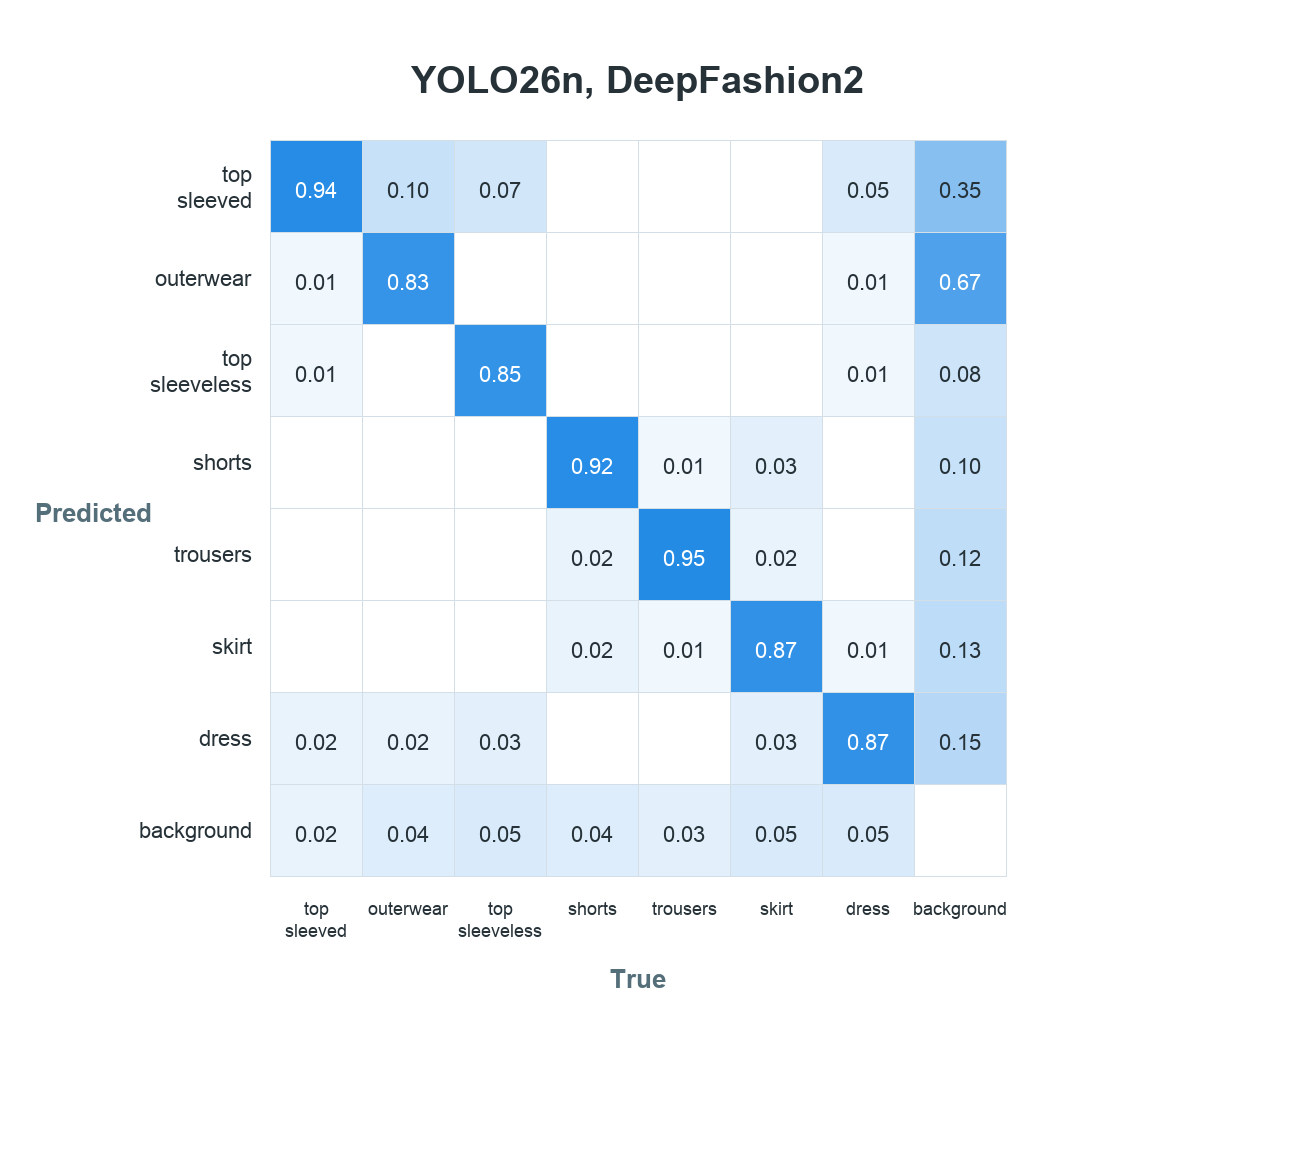
\includegraphics[width=\linewidth]{appendix/yolo26n_deepfashion2_confusion_norm.png}
\caption{YOLO26n, DeepFashion2}
\end{subfigure}
\hfill
\begin{subfigure}{0.48\linewidth}
\centering
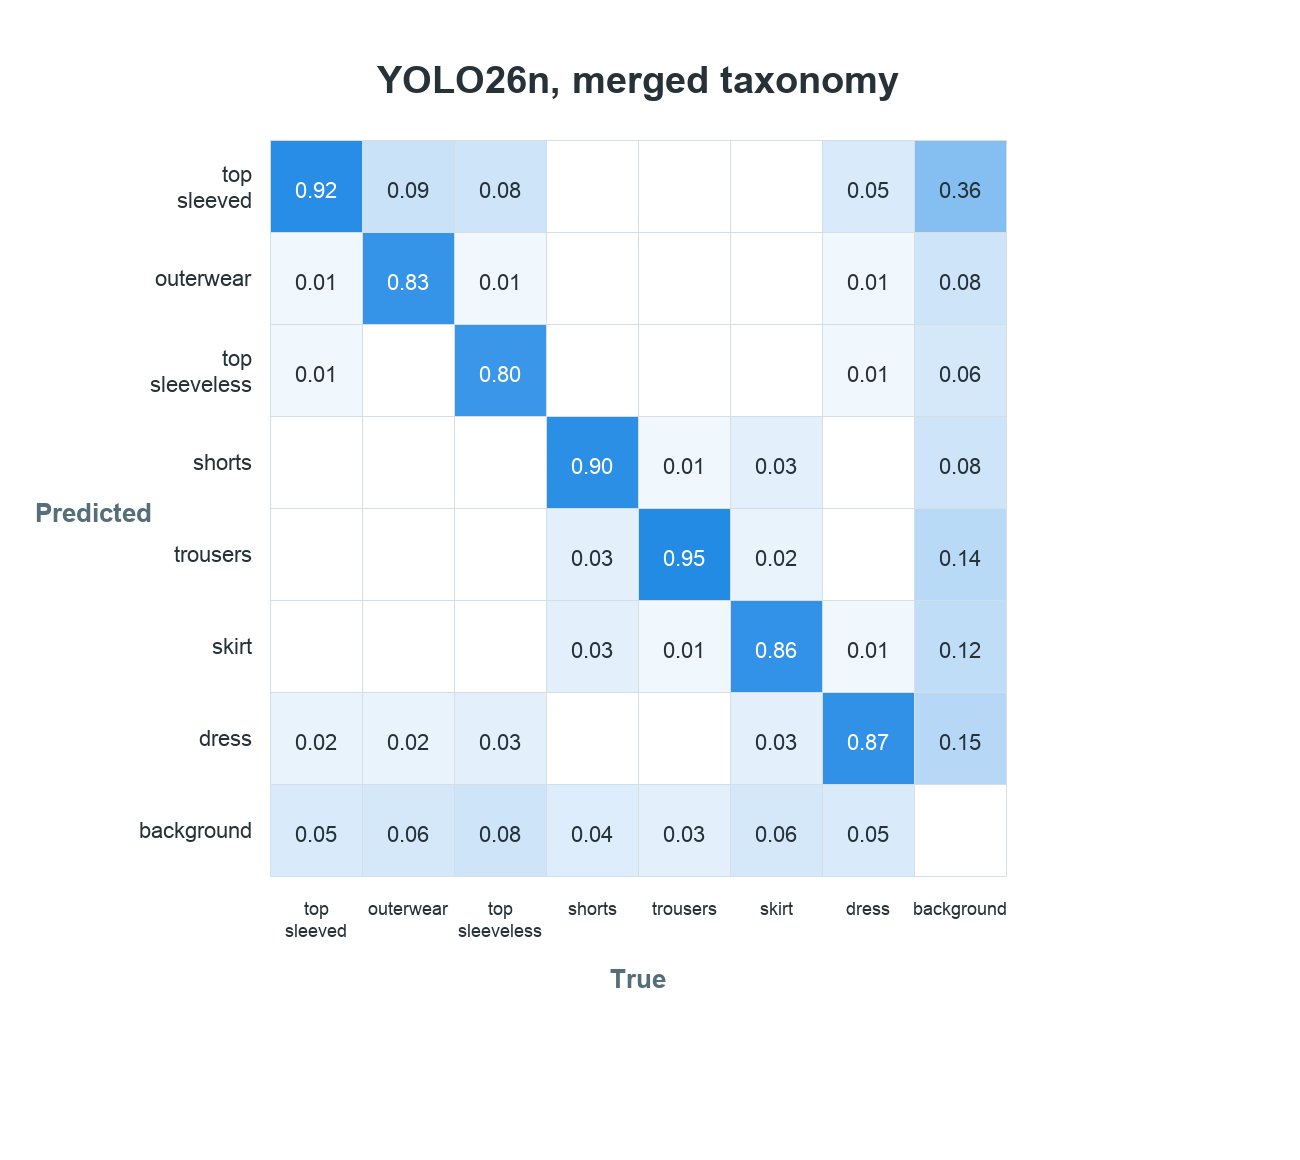
\includegraphics[width=\linewidth]{appendix/yolo26n_merged_confusion_norm.png}
\caption{YOLO26n, объединенный набор}
\end{subfigure}

\vspace{0.4cm}

\begin{subfigure}{0.48\linewidth}
\centering
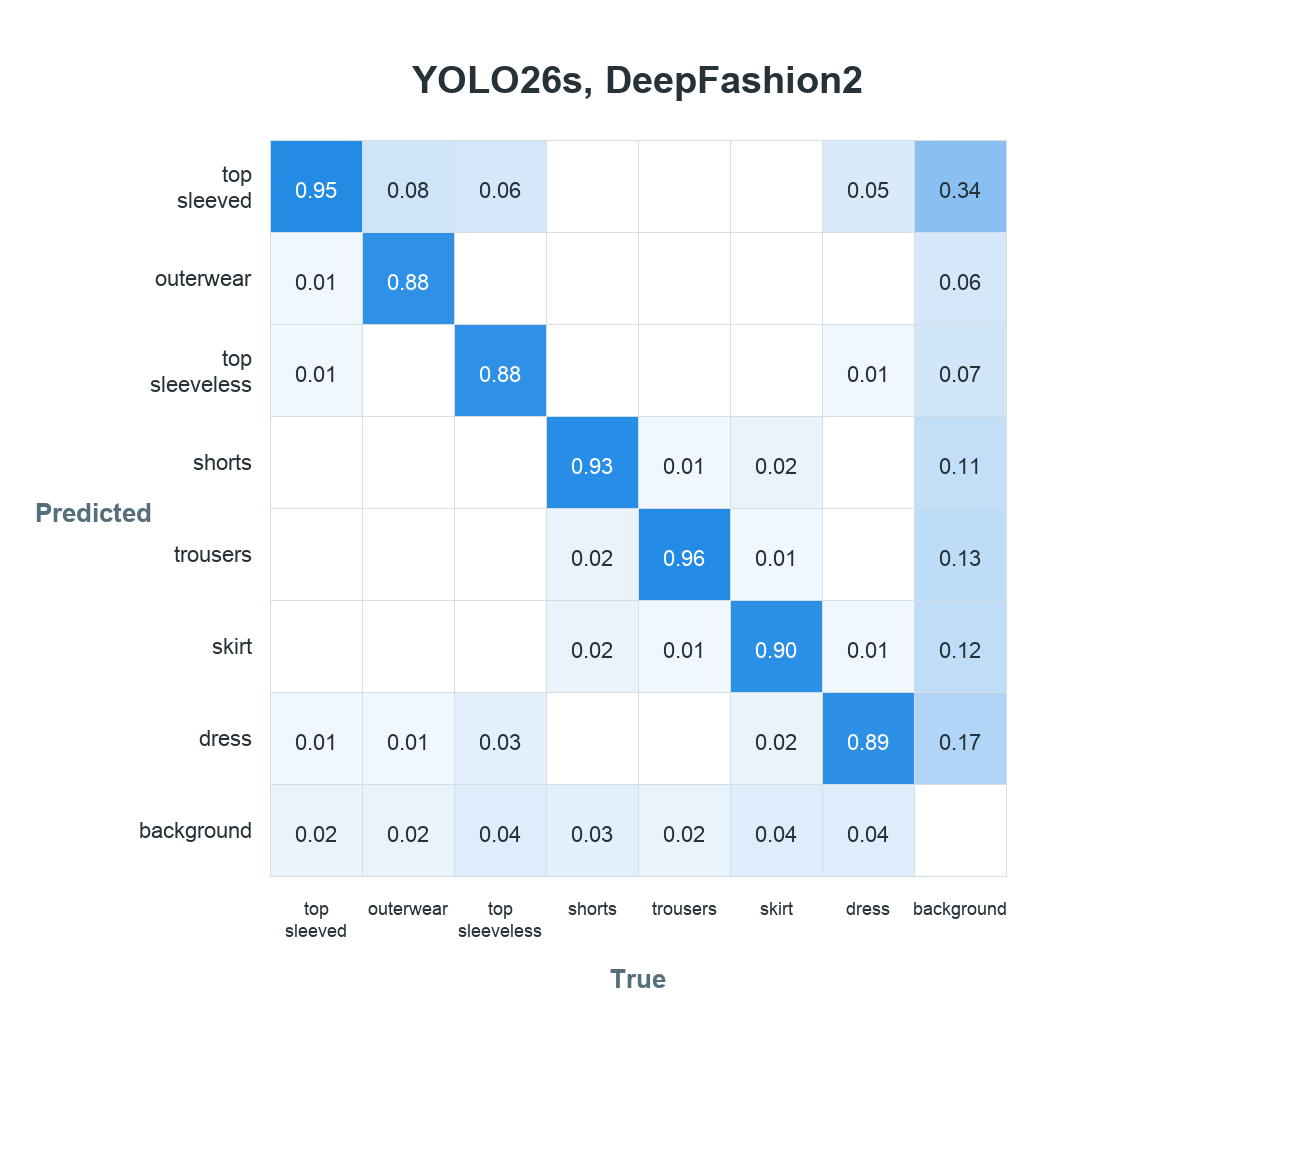
\includegraphics[width=\linewidth]{appendix/yolo26s_deepfashion2_confusion_norm.png}
\caption{YOLO26s, DeepFashion2}
\end{subfigure}
\hfill
\begin{subfigure}{0.48\linewidth}
\centering
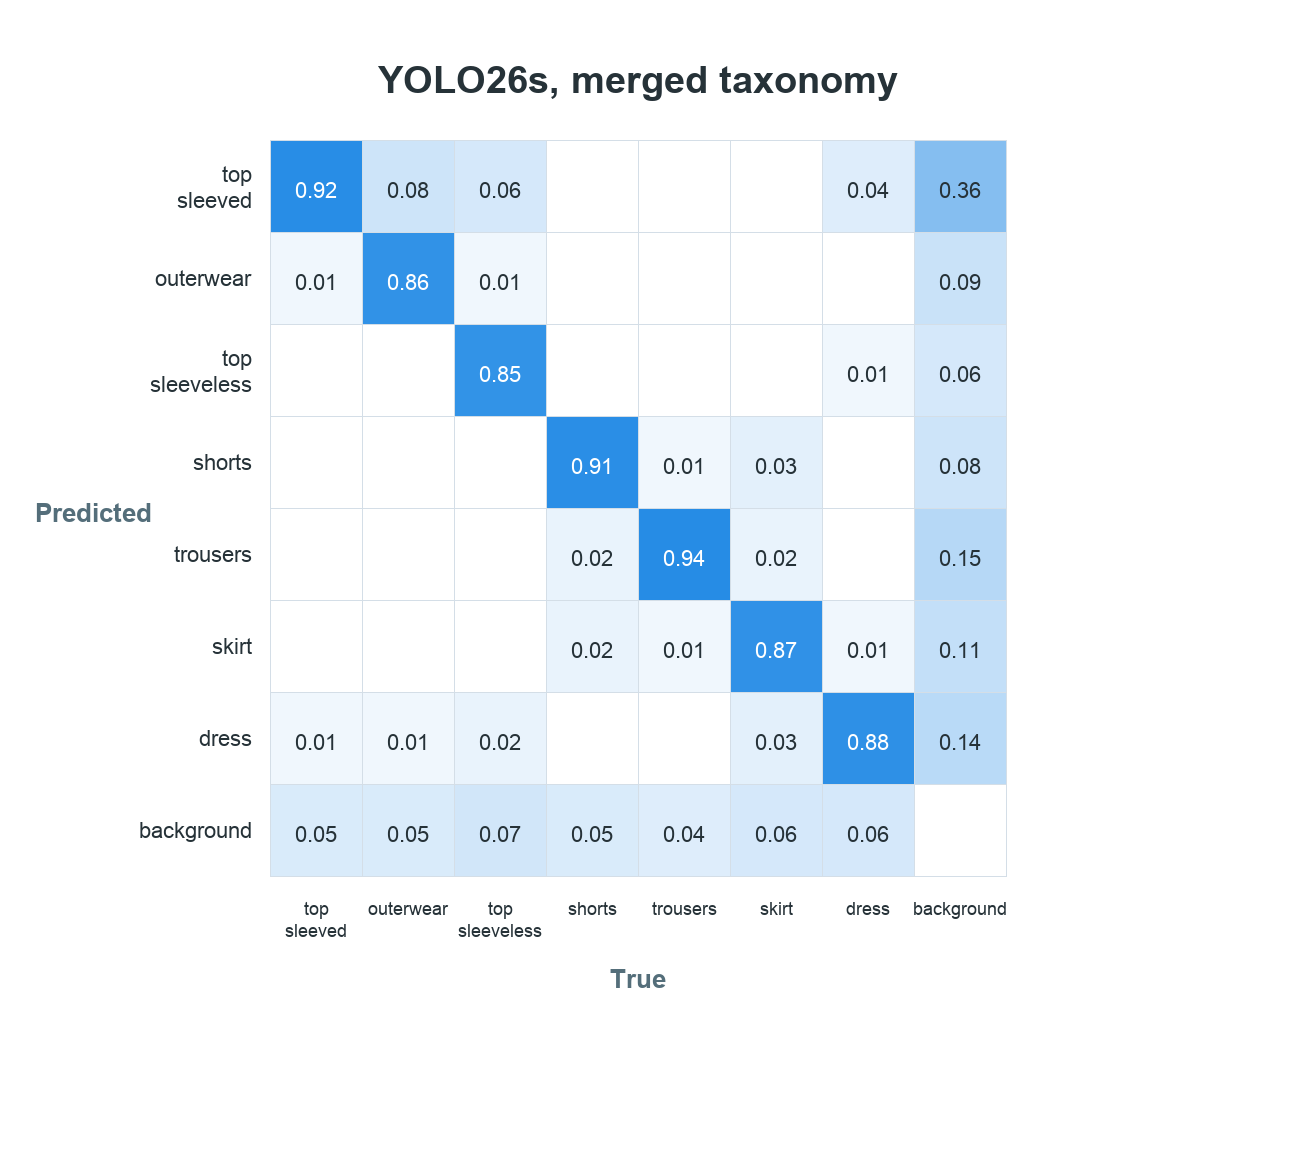
\includegraphics[width=\linewidth]{appendix/yolo26s_merged_confusion_norm.png}
\caption{YOLO26s, объединенный набор}
\end{subfigure}
\caption{Нормализованные матрицы ошибок для четырех YOLO-экспериментов.}
\label{fig:appendix_confusions}
\end{figure}

\section{Параметризованный запуск C++ benchmark}
\begin{lstlisting}[caption={Параметризованный запуск \texttt{idet\_app} для чистого latency benchmark},label={lst:experiment_config}]
idet_app \
  --mode cloth \
  --model <onnx-model> \
  --image <input-image> \
  --bind_io 1 \
  --runtime_policy 1 \
  --soft_mem_bind 1 \
  --cpu_placement latency \
  --bench_iters 30 \
  --warmup_iters 5 \
  --is_draw 0 \
  --is_dump 0 \
  --verbose 0 \
  --fixed_hw 128x128 \
  --tiles_rc 2x4 \
  --threads_intra 8 \
  --threads_inter 1 \
  --tile_omp 8
\end{lstlisting}

\section{Целевая процедура benchmark}
\begin{lstlisting}[caption={Алгоритмический benchmark-протокол grid search},label={lst:benchmark_loop}]
1. Build a full-image reference configuration.
2. For each candidate configuration:
   a. run idet_app with --is_draw 0 --is_dump 0 --verbose 0;
   b. parse p50_ms, p90_ms, p95_ms, p99_ms from stdout;
   c. reject candidates above the latency threshold;
   d. run a separate dump pass with --is_dump 1;
   e. extract Quads from stdout;
   f. compute AreaRecall, AreaPrecision, AreaF1,
      ExtraAreaRatio against the reference boxes.
3. Sort accepted candidates by p99_ms and inspect the
   Pareto trade-off between p99 latency and area quality.
\end{lstlisting}

\end{document}
